\documentclass[12pt]{ruthesis}
\usepackage{amsmath}
\usepackage{amssymb}
\usepackage{latexsym}
\usepackage{graphics}
\usepackage{slashed}
\usepackage{epsfig,epsf,rotating}
\usepackage{subfigure}
\usepackage{epsf}
\usepackage{theorem}
\usepackage{indentfirst}
\usepackage{color}
\usepackage{bm}
\usepackage{pdfpages}
\graphicspath{ {./plots/} }
\newtheorem{proposition}{Proposition}

\setcounter{secnumdepth}{3} %numbering for subsubsections

\title{Search for Top Squark via All-Hadronic Decay Channels with Heavy Object Tagging}
\ctitle{Search for Top Squark via All-Hadronic Decay Channels with Heavy Object Tagging}
\author{Matthew Cavenaugh Kilpatrick}
\department{Physics and Astronomy}
\school{Rice University}
\degree{Doctor of Philosophy}

\committee {
        Karl Ecklund, Chair \\
        Associate Professor of Physics and Astronomy \and
        Paul Padley \\
        Professor of Physics and Astronomy \and
        David Scott\\
        Noah Harding Professor
}

\address{Houston, Texas}
\donemonth{August} \doneyear{2019} \makeindex
\begin{document}

  \begin{frontmatter}
   \pagenumbering{roman}
%   \makecover
   \maketitle
   \thispagestyle{empty}
\begin{abstract}
A search for the stop quark from direct production via the all-hadronic decay channel is performed on 136.7 $\text{fb}^{-1}$ at a center-of-mass energy of 13 TeV from Run 2 of the LHC. Events are categorized into exclusive regions designed to optimize the different search topologies of the analysis. The analysis concentrates on identifying heavy object such as top quarks and W boson decays using a custom tagger for resolved tops and multivariate methods for others. A low mass spectra is enhanced using the soft b-jet transverse momentum which is typical of signal is a boosted regime with initial-state radiation. We then provide exclusion limits for each signal in the simplified models with multiple decay products.
\end{abstract}



   %\include{ack}
   \tableofcontents
   \listoffigures
   \listoftables
%   \include{ded}
  \end{frontmatter}
\pagenumbering{arabic}

\linespacing{1.5}

\newcommand*{\dphisr}{\ensuremath{\Delta\phi(t_{1,2}, \slashed{E}_{T})}}
\newcommand*{\st}{\ensuremath{\widetilde{t}} }
\newcommand*{\W}{\ensuremath{W} }
\newcommand*{\Z}{\ensuremath{Z} }
\newcommand*{\bquark}{\ensuremath{b}}
\newcommand*{\neutralino}{\ensuremath{\tilde{\chi}^{0}_{1}}}
\newcommand*{\chargino}{\ensuremath{\tilde{\chi}^{+}}}
\newcommand*{\srootb}{\ensuremath{\frac{S}{\sqrt{B}}}}
\newcommand*{\ttbar}{\ensuremath{t\bar{t}}}
\newcommand*{\met}{\ensuremath{\slashed{E}_{T}}}
\newcommand*{\ptisr}{\ensuremath{p_{T}(ISR)}}
\newcommand*{\nt}{\ensuremath{N_{t}}}
\newcommand*{\nsv}{\ensuremath{N_{SV}}}
\newcommand*{\nw}{\ensuremath{N_{W}}}
\newcommand*{\nj}{\ensuremath{N_{j}}}
\newcommand*{\nb}{\ensuremath{N_{b}}}
\newcommand*{\nrt}{\ensuremath{N_{res}}}
\newcommand*{\ptbonetwo}{\ensuremath{p_{T}(b_{12})}}
\newcommand*{\ptb}{\ensuremath{p_{T}(b)}}
\newcommand*{\dm}{\ensuremath{\Delta m}}
\newcommand*{\mtb}{\ensuremath{M_{T}(b_{1,2},\met)}}
\newcommand*{\mum}{\ensuremath{\text{}\mu}m}
\newcommand*{\cm}{\ensuremath{\text{cm}}}
\newcommand*{\GeV}{GeV}

\chapter{Introduction}
\label{ch:Intro}

The Standard Model (SM) \cite{gaillard_standard_1999} is a robust framework that allows for accurate predictions of processes involving the interactions of elementary particles. It has been developed over the course of many decades, which involved many additions such as three generations of quarks and leptons and the combination of Electromagnetism and the Weak force into a single theory. Unfortunately, we have observation for phenomena that is not explained by the SM and has eluded physicists. We present a search for a potential particle beyond the SM.
\section{Motivation}
\label{sec:Motivation}

Through various methods of experiment, we have seen that the elementary particles in the SM does not explain all of the known matter in the universe. From galactic velocity rotational curves we can deduce that the mass of galaxies must be much more than the visible matter that can be measuredmust act quite weakly with the three forces of the SM, but can still be important for gravitational effects. There are many theories beyond the SM that can explain these effects, but we will concentrate on Supersymmetry (SUSY) \cite{ramond_dual_1971, volkov_possible_1972, wess_supergauge_1974, fayet_supergauge_1975, barbieri_gauge_1982, chamseddine_locally_1982, hall_supergravity_1983, kane_study_1994, papucci_natural_2012} because of the potential for a dark matter candidate \cite{feng_dark_2010, bertone_dark_2005}, a solution to the hierarchy problem, and a potential Grand Unified Theory (GUT) \cite{georgi_unity_1974, georgi_hierarchy_1974, buras_aspects_1978}.

\begin{figure}
 	\centering
	\includegraphics[width=0.65\textwidth]{topSquarkDecay.png}
 	\caption[Top Squark Decay]{The decay of a top squark to a top quark and a neutralino.}
 	\label{topSquarkDecay} 
\end{figure}

SUSY allows for every fermion to have a bosonic partner, and vice-versa, which has all of the same quantum numbers except for a difference of $\frac{1}{2}$-integer spin. We know that since it has not yet been found that the theory must be a broken symmetry, such that the masses of the SUSY partners must have a higher mass than the SM particle. One of the main aspects of simplified SUSY, is the conservation of $R$-parity, which implies the existence of a Lightest Supersymmetric Particle (LSP). There are other models with $R$-parity violating decays \cite{barbier_r-parity-violating_2005, grossman_sneutrino_1999}, but we are not considering them. This LSP could be a potential dark matter candidate since it is stable and weakly interacting. We are interested in the neutralino, \neutralino, as the LSP, see Fig. \ref{topSquarkDecay}. 

\begin{figure}
 	\centering
	\includegraphics[width=0.65\textwidth]{HierarchyFermionLoop.png}
 	\caption[Hierarchy Fermion Loop]{The loop corrections to the Higgs boson interacting with a fermion. This is a next-to-leading order (NLO) correction to the Higgs boson mass.}
 	\label{HierarchyFermion} 
\end{figure}

The hierarchy problem is due to the loop interactions of massive quarks with the Higgs boson. This coupling causes a quadratic divergence of the Higgs mass, $m_H$, and can only be renormalized by fine tuning the coupling parameters, see Fig. \ref{HierarchyFermion}. The divergence is cutoff at the planck mass, $m_P$, known as the ultraviolet cutoff. A potential solution is the coupling of an additional bosonic particle to the quarks. This additional coupling allows for a cancellation of quadratic divergence into a logarithmic divergence, which is then renormalizable by the normal methods. This can renormalize the mass of the Higgs boson to the measured value of $m_H=125.18$ GeV \cite{chatrchyan_observation_2012, aad_observation_2012, chatrchyan_observation_2013, atlas_collaboration_combined_2015} that was discovered in 2012. Finally, SUSY also allows for a mechanism for a potential GUT. The additional superpartners allow for the three forces of the SM to converge at a large energy scale of the order $10^{16}$ GeV. We now need to develop a search strategy to try and detect these potential SUSY particles.

\section{Search}
\label{sec:search}

There are many possible searches for SUSY particles. In the Minimal Supersymmetric Standard Model (MSSM) \cite{martin_supersymmetry_1997}, it can be determined that the lightest squark that can be produced at the Large Hadron Collider (LHC) is the top quark, \st{}, which will then decay into SM particles and the LSP.  We are developing an all-hadronic search to find the \st{} which will be as inclusive as possible, so we will include all possible decay modes to get additional limits or possible detection. 

Due to the all hadronic aspect of the decay, the main backgrounds are caused by a lost lepton due to a lepton being missed for various reasons, \Znunu{} background where the missing energy is caused by the neutrinos escaping the detector, Quantum Chromodynamics (QCD) background which can be caused by the mis-measurement of jets in the event, and a rare background caused by many different types of processes which are estimated by a three lepton method of identification. We have developed 183 search regions to look for the top squark, \st{}. This is then used to get a statistical estimation of the sensitivity on the cross section for each of the production processes that we include in search. In the following chapters, we will: look into the derivation of the SM and motivations for SUSY; provide a description of the Compact Muon Solenoid (CMS) detector and the various subdetectors; describe the object selection and search strategy for the analysis; predict background estimations for each individual background; and give a description and analysis of the results and limits. 


\chapter{Supersymmetry and the Standard Model}
\label{ch:SUSY}

The fundamental theory of particle physics, known as the Standard Model (SM) can predict precise interactions between the fundamental particles in our universe. With these predictions we are able to confirm processes, but there are some aspects of the universe that have not yet been explained. In this chapter, we will analyze the Standard model and the respective models that cannot be explained.

\section{The Standard Model}
\label{sec:SM}

After decades of theoretical and experimental research the SM has been developed into a theory that explains the Electromagnetic (EM), Strong, and Weak force. The SM has not yet been able to include Gravity into the theory. With the robust theoretical and experimental methods used in the SM, we have discovered new elementary particles and predicted others. 

\section{The Fundamental Particles}

 All the matter can be explained by three kinds of elementary particles: leptons, quarks, and gauge bosons. Each of these can be distinguished by various respective properties. The leptons and quarks are fermions which are particles that have half-integer spin. The leptons are particles that only interact with the EM force, while quarks interact with the EM and Strong force. The gauge bosons are the force carries for each respective force and have integer spin. 
 
 There are three generations of leptons and quarks which are differentiated by a charge $\pm e$, the charge of an electron. The leptons have three different charged particle: electron $(e)$, muon $(\mu)$, and tau $(\tau)$. With each charged particle having a corresponding neutrino $(\nu)$ of the same flavour, see fig \ref{SMParticles}. The quarks are also separated into three generations of doublets, the down-type $(-\frac{1}{3}e)$: down $(d)$, strange $(s)$, and bottom $(b)$ and up-type $(\frac{2}{3}e)$: up $(u)$, charm $(c)$, and top $(t)$, see fig \ref{SMParticles}. Each of the quarks has a color associated with it with is analogous to an electric charge, except there are three colors charges: red, blue, and green.  

\begin{figure}
 	\centering
	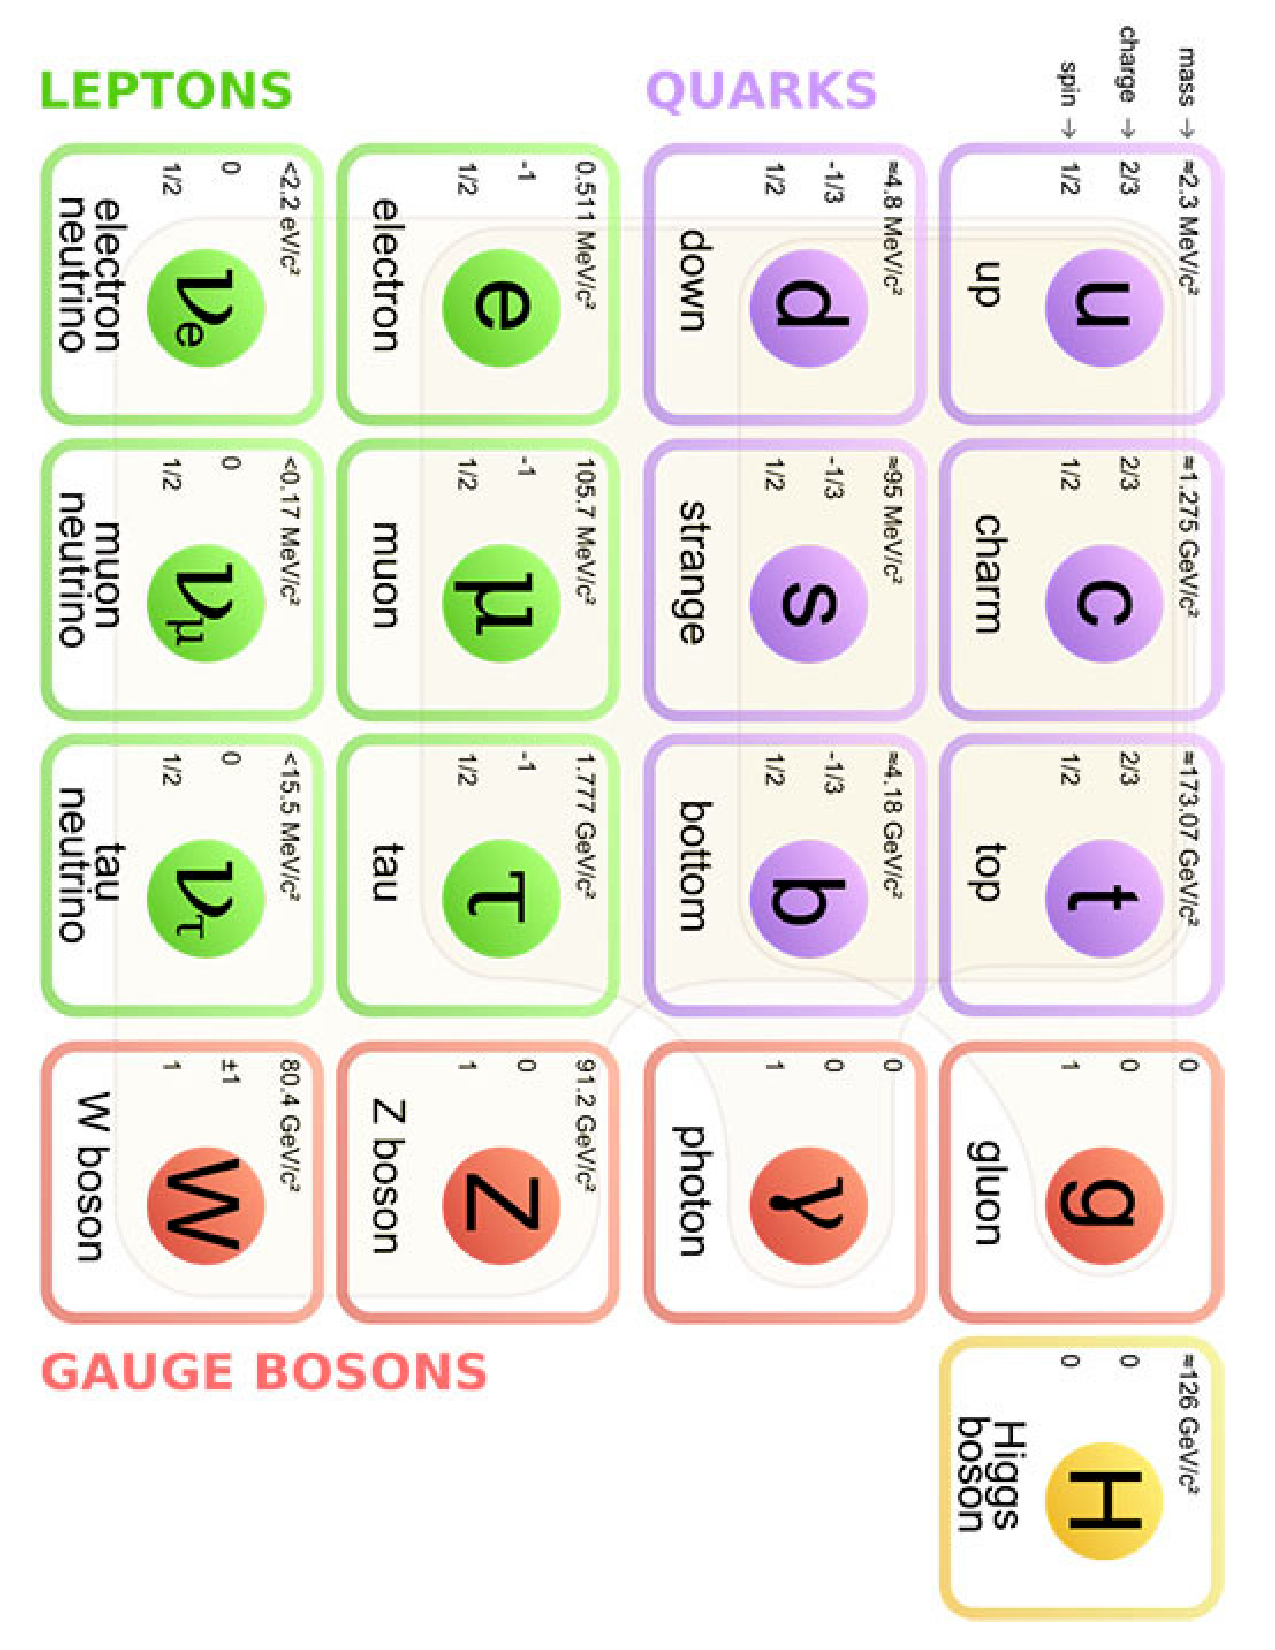
\includegraphics[width=0.75\textwidth]{StandardModel.pdf}
 	\caption{The fundamental particles of the Standard Model. There are three generations of quarks and leptons. Along with the five bosons, where four of them relate to the interactions of the three forces included in the SM: Electromagnetism, the Weak force, and the Strong force and the final being the Higgs boson which give mass to particles. }
 	\label{SMParticles} 
\end{figure}
 
 \section{Quantum Field Theory}
 \label{QFT}
 
 The interactions of all of these particles are described by the interactions of quantized fields. These fields become operators that describe the creation and annihilation of particles. Each of the fields of the SM have a corresponding boson, see fig. \ref{SMParticles}. The most well known field being the Electromagnetic (EM) field and its interactions. 
 
 Now we want to be able to write down a concise theory of the particles in the SM. The key symmetry and conservation law of the SM can be derived by starting with the Noether's Theorem.
 
 \section{Noether's Theorem}
 
 Noether's theorem states, "to each symmetry of a local Lagrangian, there corresponds a conserved current. This can be done by allowing for an infinitesimal symmetry variation. This requires the Lagrangian to be invariant under $\phi(x)\rightarrow\phi\prime(x)=\phi(x)+\alpha\Delta\phi(x)$, where $\alpha$ is infinitesimal real parameter and $\Delta\phi$ is a deformation to the field, up to a 4-divergance,
 
 \begin{equation}\label{LagrangeFluctuation}
 \mathcal{L}(x)\rightarrow\mathcal{L}(x)+\alpha\partial_\mu\mathcal{J}^\mu(x),
 \end{equation}
 
 where $\mathcal{J}^\mu$ is a current. If we apply the Euler-Lagrange equation,
 
 \begin{equation}
 \partial_\mu(\frac{\partial\mathcal{L}}{\partial(\partial_\mu\phi)})-\frac{\partial\mathcal{L}}{\partial\phi}=0,
 \end{equation}
 
 on Eqn. \ref{LagrangeFluctuation} with the addition of the fluctuation of the particle field. After some simplification we get a conserved current,
 
 \begin{equation}
 \begin{split}
 & \partial_\mu j^\mu(x)=0, \text{ where}\\
 & j^\mu(x)=\frac{\partial\mathcal{L}}{\partial(\partial_\mu\phi)}\Delta\phi-\mathcal{J}^\mu
 \end{split}
 \end{equation}.
 
 We see from the above equation that the current $j^\mu(x)$ of the Lagrangian is conserved. Now let's apply this to the particle fields of the SM.
 
 \section{QED}
 
 First, we start with the assumption that the wave function $\psi(x)$ should transform as,
 
 \begin{equation}\label{U1gauge}
 \psi(x)\rightarrow e^{i\alpha(x)}\psi(x),
 \end{equation}
 
 where $\alpha(x)$ has an arbitrary dependence on space and time. If one were to include this into the Dirac equation you would find that it is not invariant under such a local phase transformation. To include an invariace of the field, we must include a derivative, $D_\mu$, that is covariant under phase transformations,
 
 \begin{equation}\label{QEDCovariantD}
 D_\mu\equiv\partial_\mu-ieA_\mu.
 \end{equation}
 
 The covariant derivative must include the vector field $A_\mu$ which must also transform as,
  
 \begin{equation}\label{PhotonField}
 A_\mu\rightarrow A_\mu+\frac{1}{e}\partial_\mu\alpha.
 \end{equation}
 
 So after requiring that there be a local gauge transformation, we were forced to introduce a vector field $A_\mu$, called the guage field, which couples to Dirac particles in the same way as the photon field. We will think of this new field as the real photon field, which means we need to add a kinematic energy portion to the lagrangian. This kinematic term will be invariant under Eqn. \ref{PhotonField} which leads us to final final representation of the QED lagrangian which can be written down concisely as, 
 
 \begin{equation}\label{LagrangianQED}
\mathcal{L}_{QED}=\overline{\psi}(i\gamma^\mu\partial_\mu-m)\psi+e\overline{\psi}\gamma^{\mu}A_{\mu}\psi-\frac{1}{4}F^{\mu\nu}F_{\mu\nu},
 \end{equation}

where $\gamma^\mu$ are invariant tensors, $\partial_\mu$ is the partial derivative, $m$ is the mass of the particle, $\psi$ is the wave function of the particle, $A_{\mu}$ is the EM field operator, and $F^{\mu\nu}$ is the EM field tensor. Each of the parts of this equation are lorentz invariant which allows this to be true in all reference frames. This lagrangian describes the interactions of a particle and the EM field moving through spacetime. 

\section{QCD}

Let's now transition from the description of the $U(1)$ EM field to the $SU(3)$ QCD field and the transformation of quark fields. A free moving quark is described by,

\begin{equation}\label{LagrangianQCDVacuum}
\mathcal{L}_{QCD}^{vac}=\overrightarrow{q}_j(i\gamma^\mu\partial\mu-m)q_j,
\end{equation}

where $q_1, q_2,$ and $q_3$ are the three color fields. From this we want the we want to require that the field is again invariant under another local phase transformation such as,

\begin{equation}
q(x)\rightarrow Uq(x)\equiv e^{i\alpha_a(x)T_a}q(x),
\end{equation}

where $U$ is a $3\times3$ unitary matix, $T_a$ with $a=1,...,8$ are a set of linearly independent traceless $3\times3$ matrices, and $\alpha_a$ are the group parameters. Since the generators $T_a$ do not necessarily commute with each other, we can see that it is indeed non-Abelian and the commutator of can be represented as,

\begin{equation}
[T_a, T_b]=if_{abc}T_c,
\end{equation}

where $f_{abc}$ are constants. 

We need to impose $SU(3)$ local gauge invariance on Eqn. \ref{LagrangianQCDVacuum}, we allow for the following phase transformations,

\begin{equation}
\begin{split}
& q(x)\rightarrow[1+i\alpha_a(x)T_a]q(x), \\
& \partial_\mu q\rightarrow(1+i\alpha_aT_a)\partial_\mu q+iT_aq\partial_\mu\alpha_a.
\end{split}
\end{equation}

From this is seems straight forward that we can proceed in exactly the same manner as QED, which is to add

\begin{equation}
G_\mu^a\rightarrow G_\mu^a-\frac{1}{g}\partial_\mu\alpha_a, 
\end{equation}

and a covariant derivative

\begin{equation}
D_\mu=\partial_\mu+igT_aG_\mu^a.
\end{equation}

This will give us a similar lagrangian to the QED one derived above, but this is not sufficient for a non-Abelian gauge transformation and is does not produce a gauge-invariant Lagrangian. One final transformation is required for the $G_\mu^a$ fields to achieve gauge invariance, 

\begin{equation}\label{QCDGaugeTransform}
G_\mu^a\rightarrow G_\mu^a-\frac{1}{g}\partial_\mu\alpha_a-f_{abc}\alpha_b G_\mu^c,
\end{equation}

This finally give us a gauge invariant kinetic energy term for all of the $G_\mu^a$ fields and thus we can write the QCD interactions as,

\begin{equation}\label{LagrangianQCD}
\mathcal{L}_{QCD}=\overline{q}(i\gamma^\mu\partial_\mu-m)q-g(\overline{q}\gamma^\mu T_a q)G^a_\mu-\frac{1}{4}G^a_{\mu\nu}G_a^{\mu\nu}.
\end{equation}

From all of this we seem to be missing a vital part of the SM, specifically a theory for the Weakly interacting processes which is mediated by the massive bosons, $W$ and $Z$ from fig. \ref{SMParticles}. This requires the Higgs Mechanism.

\section{The Higgs Mechanism}

We are interested in the spontaneous symmetry breaking of a local $SU(2)$ gauge symmetry. We are interested in the following $SU(2)$ Lagrangian,

\begin{equation}\label{HiggsLagrangian}
\mathcal{L}=(\partial_\mu\phi)^\dagger(\partial^\mu\phi)-\mu^2\phi^\dagger\phi-\lambda(\phi^\dagger\phi)^2,
\end{equation}

with $\phi$ being a $SU(2)$ doublet of complex scalar fields

\begin{equation}
\phi=\frac{1}{2}
\begin{bmatrix}
\phi_1+i\phi_2 \\
\phi_3+i\phi_4
\end{bmatrix}
\end{equation} 

and is invariant under global the $SU(2)$ phase transformations $\phi\rightarrow e^{i\alpha_a\tau_a/2}\phi$. To allow for local invariance, we first allow for a covariant derivative

\begin{equation}
D_\mu=\partial_\mu+ig\frac{\tau_a}{2}W_\mu^a,
\end{equation}

where we now have three gauge fields, $W_\mu^a$ with $a=1,2,3$. If we assume an infanitesimal gauge transformation for the $SU(2)$ doublet $\phi(x)\rightarrow\phi'(x)=(1 +i\boldsymbol{\alpha}(x)\cdot\boldsymbol{\tau}/2)\phi(x)$, then the gauge fields will transform as

\begin{equation}\label{HiggVectorTransform}
\boldsymbol{W}_\mu\rightarrow\boldsymbol{W}_\mu-\frac{1}{g}\partial_\mu\boldsymbol{\alpha}-\boldsymbol{\alpha}\times\boldsymbol{W}_\mu,
\end{equation}

you can see that Eqn. \ref{HiggVectorTransform} is just the compact vector transform of Eqn. \ref{QCDGaugeTransform} where we have replaced the QCD gauge field with the three gauge fields $W_\mu^a$. If we include these locally invariant transformations into the above $SU(2)$ Lagrangian we get

\begin{equation}\label{HiggsInvariantL}
\mathcal{L}=(\partial_\mu\phi+ig\frac{1}{2}\boldsymbol{\tau}\cdot\boldsymbol{W}_\mu\phi)^\dagger(\partial^\mu\phi+ig\frac{1}{2}\boldsymbol{\tau}\cdot\boldsymbol{W}^\mu\phi)-\mu^2\phi^\dagger\phi+\lambda(\phi^\dagger\phi)^2-\frac{1}{4}\boldsymbol{W}_{\mu\nu}\cdot\boldsymbol{W}^{\mu\nu},
\end{equation}

where the inclusion of the gauge field kinetic term has been included at the end. The most interesting regions of this lagrangian is when $\mu^2<0$ and $\lambda>0$, where the potential has a minimum at $\phi^\dagger\phi=-\frac{\mu^2}{2\lambda}$. With this we will expand the potential around the minimum and require that

\begin{equation}
\phi_1=\phi_2=\phi_4=0, \phi_3^2=-\frac{\mu^2}{2\lambda}\equiv v^2.
\end{equation}

This is the spontaneous symmetry breaking of the $SU(2)$ symmetry, because of this we are able to substitute an expansion for the field

\begin{equation}
\phi=\sqrt{\frac{1}{2}}
\begin{bmatrix}
0 \\
v+h(x)
\end{bmatrix}
\end{equation}

With this specific transformation of the $SU(2)$ doublet and the simplification of Eqn. \ref{HiggsInvariantL}, the only remaining field is $h(x)$ which is refered to as the Higgs field. This is what is known as the Higgs Mechanism. 

We want to include the methods of the Higgs Mechanism into the weak isospin and weak hypercharge,$SU(2)_L\times U(1)_Y$, transformations of electoweak interactions. First, we need to include the coupling of the weak currents $\boldsymbol{J}_\mu$ and the gauge field $\boldsymbol{W}^\mu$ such that,

\begin{equation}
-ig\boldsymbol{J}_\mu\cdot\boldsymbol{W}^\mu=-ig\overline{\chi}_L\gamma_\mu\boldsymbol{T}\cdot\boldsymbol{W}^\mu\chi_L
\end{equation}

which is the basic interaction for the $SU(2)_L$ symmetry. Then, we also need to include the weak hypercharge current with the fourth vector boson $B^\mu$,

\begin{equation}
-i\frac{g'}{2}j_\mu^YB^\mu=-ig'\overline{\psi}\gamma_\mu\frac{Y}{2}\psi B^\mu, 
\end{equation}

here the operators $\boldsymbol{T}$ and $Y$ are generators for the $SU(2)_L$ and $U(1)_Y$ gauge transformations, respectively. Now we combine the two symmetries with the transformations of the left and right hand components of $\psi$ as

\begin{equation}
\begin{split}
\chi_L\rightarrow\chi'_L&=e^{i\boldsymbol{\alpha(x)\cdot T+i\beta(x)Y}}\chi_L, \\
\psi_R\rightarrow\psi'_R&=e^{i\beta(x)Y}\psi_R
\end{split}
\end{equation}

from this we can write down the contributions of the two gauge fields $\boldsymbol{W}_\mu^3$ and $B_\mu$ and the mising angle $\theta_W$ to find the interactions of the two neutral currents. The physical fields are thus,

\begin{equation}
-igJ_\mu^3W^{3\mu}-i\frac{g'}{2}j_\mu^YB^\mu=-iej_\mu^{em}\boldsymbol{A}^\mu-\frac{ie}{sin\theta_Wcos\theta_W}[J_\mu^3-sin^2\theta_Wj_\mu^{em}]Z^\mu.
\end{equation}

From this we can write down the Electroweak Lagrangian, for any fermion that interacts with the field. Moreover, we can formulate the Higgs mechanism, such that we can calculate the theoretical masses of the gauge bosons and fermions, such as, 

\begin{equation}
\begin{split}
& M_W=\frac{1}{2}vg \\
& M_Z=\frac{1}{2}v\sqrt{g^2+g'^2},
\end{split}
\end{equation}

but these masses cannot be predicted since the depend on the values from the chosen Higgs field. 

\subsection{The Standard Model Lagrangian}

With the inclusion of the Higgs mechanism and the formulation of a local gauge invariant Lagrangian for the Electroweak and QCD fields, we have the complete SM Lagrangian as,

\begin{equation}\label{SMLagrangian}
\begin{split}
\mathcal{L}=&-\frac{1}{4}\boldsymbol{W}_{\mu\nu}\boldsymbol{W}^{\mu\nu}-\frac{1}{4}B_{\mu\nu}B^{\mu\nu} \\
&+\overline{L}\gamma^\mu(i\partial_\mu-g\frac{1}{2}\boldsymbol{\tau}\cdot\boldsymbol{W}_\mu-g'\frac{Y}{2}B_\mu)L \\
&+\overline{R}\gamma^\mu(i\partial_\mu-g'\frac{Y}{2}B_\mu)R \\
&+\lvert(i\partial_\mu-g\frac{1}{2}\boldsymbol{\tau}\cdot\boldsymbol{W}_\mu-g'\frac{Y}{2}B_\mu)\phi\lvert^2-V(\phi) \\
&-(G_1\overline{L}\phi R+G_2\overline{L}\phi_cR+\text{hermitian conjugate}),
\end{split}
\end{equation}

where the first terms are the kinetic energies and self-interations of the $W^\pm,Z, \text{and} \gamma$ bosons, the second and third terms are the kinetic energies and interactions of the leptons and quarks with the $W^\pm,Z, \text{and} \gamma$ bosons where $L$ is a left-handed fermion doublet and $R$ is a right-handed fermion singlet. This is because the weak force only couples to left-handed fermions. The fourth term is the $W^\pm,Z,\gamma$ and Higgs masses and couplings. The final term is the lepton and quark masses and couplings to the Higgs field.  

\section{Fundamental Problems in the Standard Model}
\label{sec:SMIssues}

The SM is able to accurately and precisely describe many facits of the universe. Whether is comes to predicting the existance of a sixth quark or the confirmation of the $g - 2$ of the muon to 9 orders of magnitude. Unfortunately, there is some evidence of matter or interactions that cannot be described such as dark matter, the Hierarch problem, and a possible grand unified theory. Let's look into each of these further.

\subsection{Dark Matter}
The main motivation for Dark Matter is the difference between the visible matter and the measureable matter in the universe. This has most notibly been seen in the radial velocity of galaxies. In a galaxy which is solely made up of visible matter, matter that interacts with light, the radial velocity of stars should decrease as $1/sqrt{r}$ the further away it is from the galactic nuclei. Though measurements show the velocity becoming constant as a function of radius.

The original sutdy of this was from the galaxy NGC 1560, where the measure galactic velocity curve provided a result that was 400 times large than the visible matter in the cluster (A. H. Broeils Astron. and Astrophys. 256 19 (1992)).  To reproduce these features in models, the mass of the galaxy must be significantly more that what is seen. This implies some unseen dark matter, that still interacts with the gravitational field but not with the EM field.There is currently no such particle in the SM that has these properties.

\begin{figure}
 	\centering
	\includegraphics[width=0.5\textwidth]{Hierarchy.pdf}
 	\caption{The loop corrections to the Higgs boson interacting with a top quark and its superpartner the top squark. This is only the NLO corrections to the Higgs boson mass.}
 	\label{HiggsMass} 
\end{figure}

\subsection{Hierarchy Problem} 
The higgs boson is a beautiful solution to electroweak symmetry breaking and gives a method for particles to aqcuire mass, see Eqn. \ref{HiggsLagrangian},  and was discovery to have a measured mass, $m_{H}=125.15$ GeV. This value though is not predictable with the SM and leads to some inconsistencies when you include loop corrections. Since the higgs is strongly coupled to particles with large masses, the dominant loop correction is due to interactions with the $t$ quark. These higher order loop corrections to the higgs mass, $m_H^2$, caused by the fermionic $t$ loop, see fig \ref{HiggsMass}, are

\begin{equation} \label{HiggsDivergence}
\Delta m_{H}^{2}=-\frac{|\lambda_{f}|^{2}}{8\pi^{2}}\Lambda_{UV}^{2}+\cdot\cdot\cdot,
\end{equation}

where $\lambda_f$ is the vertex factor for the respective fermion and $\Lambda_{UV}$ is the ultraviolet momentum cutoff. The higgs boson loop corrections are highly dependent on all virtual and real particles that couple to the higgs field. From this, we can see the corrections from Eqn. \ref{HiggsDivergence} for each fermion in the SM will cause a large divergence. The quadratic divergence of the higgs mass is only renormalizable with a fine tuning of the parameters $\lambda_f$ and $\Lambda_{UV}$. This means the only way for the SM to reconcile this unfortunate fact is to have a relatively lucky cancellation of very large numbers of order $10^{32}$ with equally small numbers. Fortunately, if we add the contribution of a bosonic partner of the fermion the higgs loop corrections reduce to,

\begin{equation}
\Delta m_{H}^{2}=\frac{\lambda_{S}}{16\pi^{2}}[\Lambda_{UV}^{2} - 2m_{S}^{2}ln(\Lambda_{UV}/m_{S})+\cdot\cdot\cdot].
\label{HiggsRenormalization}
\end{equation}

With the introduction of a scalar partner to the $t$, there is a logarithmic divergence to the higgs boson mass and can be renormalized through the normal methods.

\subsection{Grand Unified Theory}

The SM is able to accurately describe three of the fundamental sources at typical energy scales, 1 to $10^{4}$ GeV, but idealy the forces would be able to merge into a single force at high energies. This has not been directly observed, but many theories, such as SUSY, predict its existance %\cite{martin_supersymmetry_1997}.

At standard energy for particle physics experiments the different in the strength of each force is quite noticeable. But it has been shown that in the SM the strengths of each force is dependent on the energy scale and it would be ideal that they converge to a single force at large energies, such as $10^16$ GeV. In fig. \ref{GUT}, we can see the extrapolated energy scales of the forces in the SM shown as the dotten line. These unfortunately, do not meet at a single point to become one force, but if we include supersymmetry into the model we get a nice convergence between the forces.

\begin{figure}
 	\centering
	\includegraphics[width=0.5\textwidth]{GUTRenormalization.png}
 	\caption{The energy dependence of the inverse gauge couple of each force in the SM (dashed line) and the MSSM (solid lines). The MSSM gives two thresholds for the sparticle mass 750 GeV and 2.5 TeV.}
 	\label{GUT} 
\end{figure}

\section{Supersymmetry}

We have seen from the above three problems that there are still more to learn than just the particles of the SM. The unexpainable features of the universe; dark matter, the hierarchy problem, and a grand unified theory have not bee attained in the SM. Forturnately, some theories have allowed for such problem to be solved. Namely the theory of supersymmetry (SUSY) which essentially states that each particle in the SM has a superpartner that has only the spin changed.


\subsection{Superpartners}
\label{sec:superpartners}

With no additional information to hint at physics at scale about the TeV range, it seems that we need a new framework for physics at the reduced Planck scale $M_{P}=(8\pi G_{Newton})^{-1/2}=2.4\times10^{18}$ GeV, which is the scale at which quantum gravitational effects become important. The ratio of $M_p/M_W$ is a strong hint that there is more physics at scales beyond the SM. We saw from the Hierarchy problem that the addition of a bosonic partner to a fermion will allow for the loop corrections to be renormalizable without fine tuning. From this we can assume that in a theory called supersymmetry, that every fermion has a bosonic partner that has all the same parameters except the spin differ by $1/2$, and vice-versa.

The partners to the fermions are donoted with a 's' in front of the name to denote it is the scalar form of the particle and the partners to the bosons have a 'ino' attached at the end, such as photino, gluino, wino, and higgsino. If the SUSY was unbroken the superpartners would have exactly the same properties as the SM pairs except their spin. This would cause a massless photino or a $m_{\tilde{e}}=0.511$ keV selectron. These particles would certainly have been seen at this point, which leads us to think that SUSY is a broken symmetry where all the superpartners have a mass that is significantly higher than their SM partners. 

Supersymmetry is broken into Chiral supermultiplets, which are fields that contain equal numbers of fermions and bosons. Each of these supermultiplets can transform and interact with each other. 

\subsection{Chirality}
\label{subsec:chiral}

Equal numbers of fermions and bosons. How does the spin change? 

\section{Minimal Supersymetric Standard Model}
\label{sec:MSSM}

Soft supersymetry breaking. 

\subsection{R Parity}
\label{subsec:rparity}

New conserved parameter known as R parity. With this is allows for a stable particle that is a dark matter candidate. Other consequences.

\section{Mass Spectrums}

Higgs boson corrections. spectrum of squarks. 







\chapter{Compact Muon Solenoid}
\label{ch:CMS}

\section{Introduction}
\label{sec:cmsIntro}

Located near Geneva, switzerland as part of the CERN collaboration. LHC provides proton beams

General CMS facts. What kind of particles is it meant to detect? What are the subdetectors? Tracker, ECAL, HCAL, superconducting solenoid, muon chambers

\section{Silicon Tracker}
\label{sec:Tracker}

\subsection{Pixel Detector}
\label{subsec:Pixel}

What is it?
Newly installed pixel detector. Larger particle flux and data rate. What is the design of the modules? How do they work?
Increased efficiency for B tagging.

\subsection{Silicon Strips}
\label{subsec:Strips}

How is it different from the pixels?

\section{Electromagnetic Calorimeter}
\label{sec:ECAL}

What kinds of particles does this detect? Mechanism?

\section{Hadronic Calorimeter}
\label{sec:HCAL}

What kinds of particles does this detect? Mechanism?

\section{Superconducting solenoid}
\label{sec:Solenoid}

Iron yoke? how strong? Purpose?

\section{Muon Chambers}
\label{sec:muCham}

What kinds of particles does this detect? Mechanism?
%\chapter{Search Strategy}
\label{ch:SearchStrategy}

\section{Physics Objects}\label{PhysObj}
There are many different types of physics objects that we are interested in when working with particle physics experiments. Since these particles have very short lifetimes, $\mathcal{O}(\text{decay})=10^{-23}$ s, we mainly interact with the decay products of the event, such as, jets $(N_j)$, heavy object tagging $(\nb, \nt, \nw, \nrt)$, missing transverse momentum (\met), scalar sum jet momentum $(H_T)$, soft-b tagging, denoted as $\nsv$, transverse mass between tagged $b$ quarks and \met{} $(m_T(b_{1,2}, \met))$, Initial State Radiation, and lepton identification. We will look into each of these objects further in this chapter.

\subsection{Jets}\label{Jets}
In an interaction whenever a quark is made it comes in pairs $(q\overline{q})$ such that the total color charge of the interaction is neutral. Typically due to conservation of momentum the quarks may originally be produced near the interaction point but will quickly start to move away from each other. Eventually the quarks will move far enough apart and will have enough potential energy in the gluon connections between them that it is then more efficient to create a new quark-antiquark $(q\overline{q})$ pair. This will continue to occur in a sequence of radiating gluons and the production of pairs of charged particles, see Fig. \ref{JetHadronization}. In the final state, the energy deposited in the HCAL is a cluster of charged particles of a radius, $\Delta R=\sqrt{\Delta\eta^2+\Delta\phi^2}$. There are many algorithms to reconstruct the jets. We are mainly interested in the anti-kT Jet algorithm \cite{cacciari_anti-ktjet_2008} method which uses the transverse momentum of the particles within a certain radius $\Delta R = 0.4 (0.8)$ for AK4(AK8) jets \cite{noauthor_https://twiki.cern.ch/twiki/bin/view/cms/jetid_nodate, noauthor_https://twiki.cern.ch/twiki/bin/view/cms/introtojec_nodate}. A charged hadron subtraction is also used to correct for the pileup, the number of collisions seen during a single proton beam crossing \cite{noauthor_pileup_2014}. Once the jets have been identified, we can analyze their respective properties to determine the likelihood of the particle it originated from, such as a $b, t, \text{ or } W$. 

\begin{figure}
 	\centering
	\includegraphics[width=0.75\textwidth]{JetHadronization.png}
 	\caption[Jet Hadronization]{A diagram of a quark pair radiating gluons that decay into more quark pairs in a process called hadronization \cite{griffiths_introduction_2008}.}
 	\label{JetHadronization} 
\end{figure}

\subsection{Heavy Object Tagging}\label{HeavyObject}
Since this search is looking for a massive particle which then decays to slightly less massive particles we need to be able to identify and distinguish between them. We use various algorithms and neural networks to identify jets from $b$ quarks, $t$ quarks, or from \W {} bosons. 

\subsubsection{B-Tagging}\label{Btagging}
Firstly, \B-tagged jets are jets that are likely to have originated from a \B{} quark. For \B{} quarks with large transverse momentum, we use a Deep Combined Secondary Vertex (DeepCSV) algorithm that involves neural networks\cite{noauthor_performance_nodate}. The medium working point recommended by the B-tag POG, corresponding to a threshold of 0.6324 0.4941, and 0.4184 for the 2016, 2017, and 2018 eras, respectively \cite{noauthor_https://twiki.cern.ch/twiki/bin/viewauth/cms/btagrecommendation2016legacy_nodate, noauthor_https://twiki.cern.ch/twiki/bin/viewauth/cms/btagrecommendation94x_nodate, noauthor_https://twiki.cern.ch/twiki/bin/viewauth/cms/btagrecommendation102x_nodate, noauthor_https://twiki.cern.ch/twiki/bin/viewauth/cms/btagsfmethods_nodate}. The medium working point is defined such that the percentage of a light jet being misidentified as a \bjet{} is 1\%.

\begin{figure}
 	\centering
	\includegraphics[width=0.75\textwidth]{TopDecayBoost.png}
 	\caption[Top Decays]{The two types of top quark reconstructions, when each decay product is easily identifiable (resolved) or when the particles are close together (boosted).}
 	\label{TopDecays} 
\end{figure}

\subsubsection{Top/W Tagging}\label{TopTagging}
The anti-kt algorithm using a distance parameter, $\Delta R=0.8$, is expected to contain the energy clusters of all of the decay product of boosted $t$ quarks, see Fig. \ref{TopDecays}, with $\pt>300$ \GeV{} or \W{} bosons with $\pt>200$ \GeV. The requirements are:
\begin{itemize}
	\item Medium working point $>0.937, 0.895, 0.895 (0.973, 0.991, 0.991)$ for boosted $t$ $(W)$ for the separate 2016, 2017, and 2018 eras, respectively.
	\item Reconstructed soft drop\cite{larkoski_soft_2014} mass: $105<m_t<210$ \GeV{} and $65<m_W<105$ \GeV.
	\item Boosted tops: $\pt=300$ \GeV, $|\eta|<2.0$ and $W$: $\pt=200$ \GeV, $|\eta|<2.0$.
\end{itemize}

There is another type of top that can be reconstructed, which is when each subjet of the top decay can be resolved into each individual jet, denoted as a resolved top, see Fig. \ref{TopDecays}. The requirements are:
\begin{itemize}
	\item Medium working point: 0.92 for all eras.
	\item $|\eta(j_{1,2,3})|<2.4$ and $b$-tag discriminator: $>0.6324, 0.4941, 0.4184$ for the separate 2016, 2017, and 2018 eras, respectively. The number of jets in the event that pass these cuts should be $\geq2$.
\end{itemize}
These object definitions, \nt, \nw, \nrt, are orthogonal to each other and are used to bin our search and control regions. 

\subsection{Missing Transverse Momentum}\label{MET}
The missing transverse momentum is the negative vector sum of the total transverse momentum measured in the detector,
\begin{equation}
\met=-\sum_{i\in\text{vis}}\overrightarrow{p}_{i, T},
\end{equation}
where the momentum runs over every visible (vis) particle in the event. Ideally, if the detector was $100\%$ efficient this quantity would always be zero due to conservation of momentum, but many things, such as detector efficiency, particles that are weakly interacting, or particles beyond the SM will cause the missing energy. Because of these, \met{} is a good discriminator for searching for physics beyond the SM \cite{noauthor_https://twiki.cern.ch/twiki/bin/view/cms/missingetrun2corrections_nodate}. 

%\subsection{MET Filters}
%Need to add MET Filters here.

\subsection{$H_T$}\label{HT}
Another interesting quantity is $H_T$, which is the scalar sum of the \pt{} of all of the jets in an event,
\begin{equation}
H_T=\sum_{i\in\text{jets}}p_{i,T}.
\end{equation}
This quantity is quite useful when trying to identify massive particles and is quite good at suppressing QCD multijet background.

\subsection{Soft $b$-Tagging}\label{SV}

The ability to identify secondary vertices is essential in searches for the top squark, see Sec. \ref{sec:Production}. Since the b quark is a long lived particle, about $10^{-12}$ seconds, it will travel many millimeters before decaying into other particles. A \B{} quark is identified during reconstruction, where the jet originating from a point separated from the primary vertex $(PV)$, known as the secondary vertex $(SV)$. The displaced vertex of the long lived $b$ quark with low \pt{} has many interesting kinematic properties that we can use to identify them, known as soft $b$-tagging. 

\begin{figure}
 	\centering
	\includegraphics[width=0.75\textwidth]{SecondaryVertex.png}
 	\caption[Secondary Vertex Diagram]{An interaction that produces a long lived particle that has a reconstructed SV.}
 	\label{SecondaryVertex} 
\end{figure}

This search also targets models that produce very soft bottom or charm quarks. A large fraction of events contain b quarks with \pt{} below the 20 GeV jet threshold which may fail to be reconstructed as jets or become b-tagged. Identification of these soft quarks improves our ability to separate potential signal events from the SM background. We therefore aim to identify $b$ or $c$ quarks based on the presence of a SV reconstructed using the Inclusive Vertex Finder (IVF) \cite{noauthor_https://twiki.cern.ch/twiki/bin/view/main/inclusivesecondaryvertexfinder_nodate, fruehwirth_new_2003}. Additional requirements on the SV observable are applied to suppress the background originating from light quarks. These selected SV may be referred to as soft $b$-tags and are constructed to be orthogonal to the jets and b-tagged jets used in this analysis. 

The requirements on each SV to pass the soft b-tagging definition are:
\begin{itemize}
	 \item The distance in the transverse plane between the SV and the PV $\leq3$ cm.
	 \item The significance of the distance, SIP3D, between the SV and the PV $\geq4$.
	 \item The pointing angle, defined as $\cos(\overrightarrow{PV,SV},\overrightarrow{p_{SV}})\geq0.98$, where $\overrightarrow{p_{SV}}$ is the total four-momentum of the tracks associated with the SV. 
	 \item The number of tracks associated with the SV is greater or equal to 3.
	 \item The \pt{} of the SV is less than 20 GeV.
\end{itemize}
Identification of soft b-quarks is necessary for potential signal region where the stop does not directly decay into a top quark and is essential for some of our search region bins. 

\subsection{Transverse Energy between $b$ quarks and \met}
We will end up dividing the search regions we are interested in into two different groups. They will be distinguished by a parameter known as the transverse mass between the leading \bjet{} and \met{} defined as:
\begin{equation}\label{TransverseMass}
\mtb=\sqrt{2\cdot\met\cdot\pt(b)(1-\cos(\slashed{E}_\phi,p_{\phi}(b)))},
\end{equation}
where \pt(b) is the momentum of the leading \bjet{} and $\slashed{E}_\phi$ and $p_{\phi}(b)$ is the $\phi$ component of the missing energy and \bjet{}, respectively. This will be used to distinguish between our low and high mass search regions, see Section \ref{SearchRegions}.


\subsection{Initial-state Radiation}\label{ISRpt}

Initial-state radiation (ISR) may be clustered into one of the large-$R$ jets clustered with a distance parameter, $\Delta R=0.8$. We use the larger radius jets to be sensitive to ISR with gluon splitting, when a jet radiates a gluon that pair produces two quarks. The ISR jet is identified as being the hardest of the large-$R$ jets with $\pt>200$ GeV which fails the loose b-tagging working point and is not identified as a top or W. This is a good parameter for jets that are neither tagged as $t$ or \W{} in the low \dm{} region of our search.
 
 \subsection{Electron and Muon Identification}\label{EleMuonID}
 There are two sets of selection criteria used in the analysis for electrons and muons. The set of criteria used to efficiently reject events with an isolated electron is done with a "Veto" ID. An electron with a Veto ID must pass the following cuts:
 \begin{itemize}
	 \item $|\Delta\eta|<0.007(0.01),|\Delta\phi|<0.8(0.7)$ for the electrons (muons).
	 \item $\sigma_{i\eta i\eta}<0.01(0.03)$ for the electrons (muons).
	 \item $H/E<0.15(N/A)$.
	 \item $\text{PF isolation}/\pt(\text{cone } \Delta R=0.3)<0.15(0.15)$ for the electrons (muons).
	 \item $|d_{0}|<0.04(0.04),|d_Z|<0.2(0.2)$ for the electrons (muons).
 \end{itemize}
 for the barrel and endcap regions of the detector, where $H/E$ is the ratio of hadronic energy over electromagnetic energy. This veto ID is chosen such that the search region is most likely to be devoid of electrons, since it has a 95\% efficiency \cite{noauthor_https://twiki.cern.ch/twiki/bin/view/cms/cutbasedelectronidentificationrun2_nodate}.
 
 We use the Loose muon definition recommended by the Muon POG for the purposes of the muon veto \cite{noauthor_https://twiki.cern.ch/twiki/bin/view/cmspublic/swguidemuonidloose_muon_nodate}. A Loose muon is identified as a Particle Flow (PF)\cite{noauthor_cms_nodate} muon and can be either a global muon or an arbitrated tracker muon. Only candidates with transverse (longitudinal) impact parameter $|d_0|<0.2$ cm $(|d_z|<0.5 \text{cm},)$ with respect to the primary vertex, are considered. The electron and muon IDs are used in the definition of the Lost Lepton background which will be expanded upon further in Section \ref{sec:LL}. 
 
\subsection{Tau Identification}\label{TauID}
The Tau ID has been studied extensively in tests which looked into the custom MVA \cite{roe_boosted_2004, hoecker_tmva_2007, bravo_search_2015} similar to the one used in Ref. \cite{cms_collaboration_search_2016}, a cut-based IsoTrack method, and Tau POG MVA method of identifying hadronically decaying taus. The methods which provide the best improvement to the efficiency of identifying taus with a small fake rate is the combination of IsoTrack and Tau POG MVA. With the inclusion of the combined method for identifying hadronically decaying taus, the veto percentage is $\approx29.0\%(7.2\%)$ with an efficiency of the veto of $\approx49.1\%(22.6\%)$ for SM background (signal), see Appendix. \ref{sec:TauMVA}. 

For the IsoTrack method we require the following:
\begin{itemize}
	\item $\pt\geq5(10) \GeV, \text{iso}\leq0.2(0.1)$ for electrons and muons(pions);
	\item $m_T(\text{IsoTrack},\met)<100 \GeV$;
\end{itemize}
where $m_T(\text{IsoTrack},\met)$ is the transverse mass between the IsoTrack and \met. For the Tau POG method we require:
\begin{itemize}
	\item $\pt\geq20 \GeV, |\eta|<2.4$;
	\item idDecayMode, a booleon to identify hadronically decaying taus; and
	\item Medium working point.
\end{itemize}
With the inclusion of the separate electron/muon IDs and the combined IsoTrack + TauPOG IDs we have a method to efficiently veto leptons from our search region.

\section{Samples}\label{Samples}
\label{sec:samples}
The primary dataset used for this analysis is the MET dataset.
% Are the datasets described online somewhere? Put a citation link pointing to it. You could even add a footnote like \footnote{All of the datasets discussed in this section are described in more detail at \href{http://www.link}{link}. Include \usepackage{hyperref}
% Actually, there is no convenient link for Run 2 datasets, just a pdf for now. This should be updated once there is something better available.
% ~\footnote{All of the datasets discussed in this section are described in more detail at \href{http://hermine.web.cern.ch/hermine/CMS/CMS_PDs_733ntuples_7e33menu_HKWoehri.pdf}{\emph{2015 Primary Dataset Definitions}}.}
It contains events triggered by the HLT paths HLT\_PFMETx\_PFMHTx\_IDTight and HLT\_PFMET\\*NoMux\_PFMHTNoMux\_IDTight where x = 100, 110, 120, 130, and 140. The logical OR of these triggers is used to select the search sample. 
 For studies of single- and dilepton control regions, we use the SingleMuon, SingleElectron, DoubleMuon, and DoubleEG datasets. The JetHT dataset is also used for studies of \W/topq-tagging. The SinglePhoton dataset is used to define a control region with a selected photon that is used together with \Zll~  samples for the prediction of the SM background originating from \Znunu~events. Table~\ref{tab:datasets} lists all datasets together with the specific HLT paths of the triggers that were used for the selection of events. In cases where there are inefficiencies due to the use of isolated triggers, a suite of triggers is used to recover efficiency wherever possible. The datasets correspond to the full Run 2 dataset are: ``Run2016B", ``Run2016C", ``Run2016D", ``Run2016E", ``Run2016F", ``Run2016G", ``Run2016H", ``Run2017B", ``Run2017C", ``Run2017D", ``Run2017E", ``Run2017F", ``Run2018A", ``Run2018B", ``Run2018C", and ``Run2018D" acquisition eras with a total luminosity of \datalumi, Table \ref{tab:datasets}.

\begin{table}[!ht]
\begin{center}
\small
%\hskip-0.5cm
\resizebox*{1\textwidth}{!}{
\begin{tabular}{|l|l|}
\hline
Primary dataset & HLT path \\
%\hline
%/JetHT/Run2016B-PromptReco-v1/MINIAOD & HLT\_PFHT800 \\
%/JetHT/Run2016B-PromptReco-v2/MINIAOD & HLT\_PFHT800 \\
\hline
\multicolumn{2}{|c|}{Search sample} \\
\hline
\multirow{10}{*}{MET} & HLT\_PFMET100\_PFMHT100\_IDTight OR HLT\_PFMETNoMu100\_PFMHTNoMu100\_IDTight OR \\
 & HLT\_PFMET110\_PFMHT110\_IDTight OR HLT\_PFMETNoMu110\_PFMHTNoMu110\_IDTight OR \\
 & HLT\_PFMET120\_PFMHT120\_IDTight OR HLT\_PFMETNoMu120\_PFMHTNoMu120\_IDTight OR \\
 & HLT\_PFMET130\_PFMHT130\_IDTight OR HLT\_PFMETNoMu130\_PFMHTNoMu130\_IDTight OR \\
 & HLT\_PFMET140\_PFMHT140\_IDTight OR HLT\_PFMETNoMu140\_PFMHTNoMu140\_IDTight OR \\
 & HLT\_PFMET100\_PFMHT100\_IDTight\_PFHT60 OR HLT\_PFMETNoMu100\_PFMHTNoMu100\_IDTight\_PFHT60 OR \\
 & HLT\_PFMET110\_PFMHT110\_IDTight\_PFHT60 OR HLT\_PFMETNoMu110\_PFMHTNoMu110\_IDTight\_PFHT60 OR \\
 & HLT\_PFMET120\_PFMHT120\_IDTight\_PFHT60 OR HLT\_PFMETNoMu120\_PFMHTNoMu120\_IDTight\_PFHT60 OR \\
 & HLT\_PFMET130\_PFMHT130\_IDTight\_PFHT60 OR HLT\_PFMETNoMu130\_PFMHTNoMu130\_IDTight\_PFHT60 OR \\
 & HLT\_PFMET140\_PFMHT140\_IDTight\_PFHT60 OR HLT\_PFMETNoMu140\_PFMHTNoMu140\_IDTight\_PFHT60 \\
\hline
\multicolumn{2}{|c|}{Single-lepton control sample} \\
\hline
\multirow{3}{*}{SingleMuon} & HLT\_IsoMu20 OR HLT\_IsoTkMu20 OR HLT\_IsoMu22 OR HLT\_IsoTkMu22 OR HLT\_IsoMu24 OR HLT\_IsoTkMu24 OR \\ 
 & HLT\_IsoMu27 OR HLT\_IsoTkMu27 OR HLT\_IsoMu22\_eta2p1 OR HLT\_IsoMu24\_eta2p1 OR \\
 & HLT\_IsoTkMu22 OR HLT\_IsoTkMu24 OR HLT\_Mu50 OR HLT\_Mu55 OR \\ 
 \hline
\multirow{5}{*}{SingleElectron} & HLT\_Ele105\_CaloIdVT\_GsfTrkIdT OR HLT\_Ele115\_CaloIdVT\_GsfTrkIdT OR HLT\_Ele135\_CaloIdVT\_GsfTrkIdT OR HLT\_Ele145\_CaloIdVT\_GsfTrkIdT OR \\
 & HLT\_Ele25\_eta2p1\_WPTight\_Gsf OR HLT\_Ele20\_eta2p1\_WPLoose\_Gsf OR HLT\_Ele27\_eta2p1\_WPLoose\_Gsf OR \\ 
 & HLT\_Ele27\_WPTight\_Gsf OR HLT\_Ele35\_WPTight\_Gsf OR HLT\_Ele20\_WPLoose\_Gsf OR HLT\_Ele45\_WPLoose\_Gsf OR\\
 & Ele23\_Ele12\_CaloIdL\_TrackIdL\_IsoVL OR Ele23\_Ele12\_CaloIdL\_TrackIdL\_IsoVL\_DZ OR \\
 & DoubleEle33\_CaloIdL\_GsfTrkIdVL OR DoubleEle33\_CaloIdL\_GsfTrkIdVL\_MW OR DoubleEle25\_CaloIdL\_MW OR DoubleEle33\_CaloIdL\_MW\\
 \hline
\multirow{2}{*}{MET} & HLT\_PFMET110\_PFMHT110\_IDTight OR HLT\_PFMETNoMu110\_PFMHTNoMu110\_IDTight \\
 & HLT\_PFMET120\_PFMHT120\_IDTight OR HLT\_PFMETNoMu120\_PFMHTNoMu120\_IDTight \\
 \hline
JetHT & HLT\_CaloJet500\_NoJetID \\
DoubleEG & HLT\_ECALHT800 \\
\hline
\multicolumn{2}{|c|}{Dilepton control sample} \\
\hline
\multirow{4}{*}{DoubleMuon} & (all eras) kHLT\_Mu30\_TkMu11 \\
 & (Before era H) HLT\_Mu17\_TrkIsoVVL\_Mu8\_TrkIsoVVL OR HLT\_Mu17\_TrkIsoVVL\_TkMu8\_TrkIsoVVL \\
 & (Era H) HLT\_Mu17\_TrkIsoVVL\_Mu8\_TrkIsoVVL\_DZ OR HLT\_Mu17\_TrkIsoVVL\_TkMu8\_TrkIsoVVL\_DZ \\
 & (Era H) HLT\_TkMu17\_TrkIsoVVL\_TkMu8\_TrkIsoVVL\_DZ \\
SingleMuon & HLT\_Mu50 OR HLT\_TkMu50\\
DoubleEG & HLT\_Ele23\_Ele12\_CaloIdL\_TrackIdL\_IsoVL\_DZ OR HLT\_DoubleEle33\_CaloIdL\_GsfTrkIdVL\_MW \\
SingleElectron & HLT\_Ele115\_CaloIdVT\_GsfTrkIdT \\
\hline
\multicolumn{2}{|c|}{Photon control sample} \\
\hline
SinglePhoton & HLT\_Photon175 OR HLT\_Photon200 \\
\hline
\end{tabular}
}
\end{center}
\caption[Data Samples]{\label{tab:datasets}Primary datasets used for the analysis and the HLT paths of the corresponding triggers. Datasets from Run2016 are ``ReReco" legacy datasets from the 17Jul2018 re-reconstruction, Run2017 is from 31Mar2018 re-reconstruction, and Run2018 Run ``A" to ``C" are re-reconstruction while Run ``D" is promptreco.}
\end{table}

The simulated samples used in this analysis, all of which are listed in Table~\ref{tab:samples} and \ref{tab:signals}, were produced as part of the ``Summer16", ``Fall17", and ``Autumn18" Monte Carlo production campaign for Run 2 in the ``NanoAOD" data format.

\begin{table}[!htp]
\begin{center}
\small
%\hskip-1.0cm
\resizebox*{1\textwidth}{!}{
\begin{tabular}{|l|l|l|l|}
\hline
Process & Generator & Dataset & Cross section [pb]\\
\hline
\multicolumn{4}{|c|}{SM processes}\\
\hline
$\ttbar, 1\ell$ & \textsc{madgraph} & /TTJets\_SingleLeptFromT\_TuneCUETP8M1\_13TeV-madgraphMLM-pythia8/$<$proc$>$ & 182.18 \\
     &  & /TTJets\_SingleLeptFromTbar\_TuneCUETP8M1\_13TeV-madgraphMLM-pythia8/$<$proc$>$ & 182.18 \\
$\ttbar, 2\ell$ & \textsc{madgraph} & /TTJets\_DiLept\_TuneCUETP8M1\_13TeV-madgraphMLM-pythia8/$<$proc$>$ & 87.31 \\
\hline
$\ttbar, \Ht$ & \textsc{madgraph} & /TTJets\_HT-600to800\_TuneCUETP8M1\_13TeV-madgraphMLM-pythia8/$<$proc$>$ & 2.76 \\
     &  & /TTJets\_HT-800to1200\_TuneCUETP8M1\_13TeV-madgraphMLM-pythia8/$<$proc$>$ & 1.1156 \\
     &  & /TTJets\_HT-1200to2500\_TuneCUETP8M1\_13TeV-madgraphMLM-pythia8/$<$proc$>$ & 0.19775 \\
     &  & /TTJets\_HT-2500toInf\_TuneCUETP8M1\_13TeV-madgraphMLM-pythia8/$<$proc$>$ & 0.00239 \\
\hline
ttZ & \textsc{amcatnlo} & /TTZToLLNuNu\_M-10\_TuneCUETP8M1\_13TeV-amcatnlo-pythia8/$<$proc$>$ & 0.2529 \\
     & \textsc{amcatnlo} & /TTZToQQ\_TuneCUETP8M1\_13TeV-amcatnlo-pythia8/$<$proc$>$ & 0.5297 \\
\hline
tZq & \textsc{amcatnlo} & /tZq\_ll\_4f\_13TeV-amcatnlo-pythia8\_TuneCUETP8M1/$<$proc$>$ & 0.0758 \\
\hline
tW & \textsc{madgraph} & /ST\_tWll\_5f\_LO\_13TeV-MadGraph-pythia8/$<$proc$>$ & 0.01104 \\
 & \textsc{madgraph} & /ST\_tWnunu\_5f\_LO\_13TeV-MadGraph-pythia8/$<$proc$>$ & 0.02122 \\
\hline
ttW & \textsc{amcatnlo} & /TTWJetsToLNu\_TuneCUETP8M1\_13TeV-amcatnloFXFX-madspin-pythia8/$<$proc$>$ & 0.2043 \\
     & \textsc{amcatnlo} & /TTWJetsToQQ\_TuneCUETP8M1\_13TeV-amcatnloFXFX-madspin-pythia8/$<$proc$>$ & 0.4062 \\
\hline
t\W & \textsc{powheg} & /ST\_tW\_top\_5f\_NoFullyHadronicDecays\_13TeV-powheg\_TuneCUETP8M1/$<$proc$>$ & 16.295 \\
       & \textsc{powheg} & /ST\_tW\_top\_5f\_inclusiveDecays\_13TeV-powheg-pythia8\_TuneCUETP8M1/$<$proc$>$ & 35.85 \\
       & \textsc{powheg} & /ST\_tW\_antitop\_5f\_NoFullyHadronicDecays\_13TeV-powheg\_TuneCUETP8M1/$<$proc$>$ & 16.295 \\
       & \textsc{powheg} & /ST\_tW\_antitop\_5f\_inclusiveDecays\_13TeV-powheg-pythia8\_TuneCUETP8M1/$<$proc$>$ & 35.85 \\
t\W, t-channel & \textsc{amcatnlo} & /ST\_t-channel\_top\_4f\_inclusiveDecays\_13TeV-powhegV2-madspin-pythia8\_TuneCUETP8M1/$<$proc$>$ & 136.065 \\
                        & \textsc{amcatnlo} & /ST\_t-channel\_antitop\_4f\_inclusiveDecays\_13TeV-powhegV2-madspin-pythia8\_TuneCUETP8M1/$<$proc$>$ & 80.97 \\
t\W, s-channel & \textsc{amcatnlo} & /ST\_s-channel\_4f\_inclusiveDecays\_13TeV-amcatnlo-pythia8\_TuneCUETP8M1/$<$proc$>$ & 3.362 \\
\hline
%\W+jets & \textsc{amcatnlo} & /WJetsToLNu\_TuneCUETP8M1\_13TeV-amcatnloFXFX-pythia8/$<$proc$>$ & 61526.7 \\
\W+jets & \textsc{madgraph}, HT bins & /WJetsToLNu\_HT-70To100\_TuneCUETP8M1\_13TeV-madgraphMLM-pythia8/$<$proc$>$ & 1353 \\
    & & /WJetsToLNu\_HT-100To200\_TuneCUETP8M1\_13TeV-madgraphMLM-pythia8/$<$proc$>$ & 1345 \\
    & & /WJetsToLNu\_HT-200To400\_TuneCUETP8M1\_13TeV-madgraphMLM-pythia8/$<$proc$>$ & 359.7 \\
    & & /WJetsToLNu\_HT-400To600\_TuneCUETP8M1\_13TeV-madgraphMLM-pythia8/$<$proc$>$ & 48.91 \\
    & & /WJetsToLNu\_HT-600To800\_TuneCUETP8M1\_13TeV-madgraphMLM-pythia8/$<$proc$>$ & 12.05 \\
    & & /WJetsToLNu\_HT-800To1200\_TuneCUETP8M1\_13TeV-madgraphMLM-pythia8/$<$proc$>$ & 5.501 \\
    & & /WJetsToLNu\_HT-1200To2500\_TuneCUETP8M1\_13TeV-madgraphMLM-pythia8/$<$proc$>$ & 1.329 \\
    & & /WJetsToLNu\_HT-2500ToInf\_TuneCUETP8M1\_13TeV-madgraphMLM-pythia8/$<$proc$>$ & 0.03216 \\
\hline
 \Znunu & \textsc{madgraph}, HT bins & /ZJetsToNuNu\_HT-100To200\_13TeV-madgraph/$<$proc$>$ & 280.35 \\
    & & /ZJetsToNuNu\_HT-200To400\_13TeV-madgraph/$<$proc$>$ & 77.67 \\
    & & /ZJetsToNuNu\_HT-400To600\_13TeV-madgraph/$<$proc$>$ & 10.73 \\
    & & /ZJetsToNuNu\_HT-600To800\_13TeV-madgraph/$<$proc$>$ & 2.559 \\
    & & /ZJetsToNuNu\_HT-800To1200\_13TeV-madgraph/$<$proc$>$ & 1.1796 \\
    & & /ZJetsToNuNu\_HT-1200To2500\_13TeV-madgraph/$<$proc$>$ & 0.28833 \\
    & & /ZJetsToNuNu\_HT-2500ToInf\_13TeV-madgraph/$<$proc$>$ & 0.006945 \\
\hline
QCD & \textsc{madgraph}, HT bins & /QCD\_HT100to200\_TuneCUETP8M1\_13TeV-madgraphMLM-pythia8/$<$proc$>$ & 27990000 \\
    & & /QCD\_HT200to300\_TuneCUETP8M1\_13TeV-madgraphMLM-pythia8/$<$proc$>$ & 1712000 \\
    & & /QCD\_HT300to500\_TuneCUETP8M1\_13TeV-madgraphMLM-pythia8/$<$proc$>$ & 347700 \\
    & & /QCD\_HT500to700\_TuneCUETP8M1\_13TeV-madgraphMLM-pythia8/$<$proc$>$ & 32100 \\
    & & /QCD\_HT700to1000\_TuneCUETP8M1\_13TeV-madgraphMLM-pythia8/$<$proc$>$ & 6831 \\
    & & /QCD\_HT1000to1500\_TuneCUETP8M1\_13TeV-madgraphMLM-pythia8/$<$proc$>$ & 1207 \\
    & & /QCD\_HT1500to2000\_TuneCUETP8M1\_13TeV-madgraphMLM-pythia8/$<$proc$>$ & 119.9 \\
    & & /QCD\_HT2000toInf\_TuneCUETP8M1\_13TeV-madgraphMLM-pythia8/$<$proc$>$ & 25.24 \\
\hline
gg+jets & \textsc{madgraph}, HT bins & /GJets\_HT-100To200\_TuneCUETP8M1\_13TeV-madgraphMLM-pythia8/$<$proc$>$ & 5391.0 \\
    & & /GJets\_HT-200To400\_TuneCUETP8M1\_13TeV-madgraphMLM-pythia8/$<$proc$>$ & 1168.0 \\
    & & /GJets\_HT-400To600\_TuneCUETP8M1\_13TeV-madgraphMLM-pythia8/$<$proc$>$ & 132.5 \\
    & & /GJets\_HT-600ToInf\_TuneCUETP8M1\_13TeV-madgraphMLM-pythia8/$<$proc$>$ & 44.05 \\
\hline
\ttbar gg+jets & \textsc{amcatnlo} & /TTGJets\_TuneCUETP8M1\_13TeV-amcatnloFXFX-madspin-pythia8/$<$proc$>$ & 3.697 \\
\hline
DY+jets & \textsc{madgraph}, HT bins & /DYJetsToLL\_M-50\_HT-70to100\_TuneCUETP8M1\_13TeV-madgraphMLM-pythia8/$<$proc$>$ & 169.9 \\
    & & /DYJetsToLL\_M-50\_HT-100to200\_TuneCUETP8M1\_13TeV-madgraphMLM-pythia8/$<$proc$>$ & 147.4 \\
    & & /DYJetsToLL\_M-50\_HT-200to400\_TuneCUETP8M1\_13TeV-madgraphMLM-pythia8/$<$proc$>$ & 40.99 \\
    & & /DYJetsToLL\_M-50\_HT-400to600\_TuneCUETP8M1\_13TeV-madgraphMLM-pythia8/$<$proc$>$ & 5.678 \\
    & & /DYJetsToLL\_M-50\_HT-600to800\_TuneCUETP8M1\_13TeV-madgraphMLM-pythia8/$<$proc$>$ & 1.367 \\
    & & /DYJetsToLL\_M-50\_HT-800to1200\_TuneCUETP8M1\_13TeV-madgraphMLM-pythia8/$<$proc$>$ & 0.6304 \\
    & & /DYJetsToLL\_M-50\_HT-1200to2500\_TuneCUETP8M1\_13TeV-madgraphMLM-pythia8/$<$proc$>$ & 0.1514 \\
    & & /DYJetsToLL\_M-50\_HT-2500toInf\_TuneCUETP8M1\_13TeV-madgraphMLM-pythia8/$<$proc$>$ & 0.003565 \\
\hline
\W\W & \textsc{powheg} & /WWTo2L2Nu\_13TeV-powheg/$<$proc$>$ & 12.178 \\
     & \textsc{powheg} & /WWToLNuQQ\_13TeV-powheg/$<$proc$>$ & 49.997 \\
     & \textsc{powheg} & /WWTo4Q\_13TeV-powheg/$<$proc$>$ & 51.723 \\
\hline
\W\Z & \textsc{amcatnlo} & /WZTo1L1Nu2Q\_13TeV\_amcatnloFXFX\_madspin\_pythia8/$<$proc$>$ & 10.71 \\
     & \textsc{powheg} & /WZTo3LNu\_TuneCUETP8M1\_13TeV-powheg-pythia8/$<$proc$>$ & 4.42965 \\
     & \textsc{amcatnlo} & /WZTo2L2Q\_13TeV\_amcatnloFXFX\_madspin\_pythia8/$<$proc$>$ & 5.595 \\
     & \textsc{amcatnlo} & /WZTo1L3Nu\_13TeV\_amcatnloFXFX\_madspin\_pythia8/$<$proc$>$ & 3.033 \\
\hline
\Z\Z & \textsc{amcatnlo} & /ZZTo2Q2Nu\_13TeV\_amcatnloFXFX\_madspin\_pythia8/$<$proc$>$ & 4.033 \\
     & \textsc{amcatnlo} & /ZZTo2L2Q\_13TeV\_amcatnloFXFX\_madspin\_pythia8/$<$proc$>$ & 3.22 \\
     & \textsc{powheg} & /ZZTo2L2Nu\_13TeV\_powheg\_pythia8/$<$proc$>$ & 0.564 \\
     & \textsc{powheg} & /ZZTo4L\_13TeV\_powheg\_pythia8/$<$proc$>$ & 1.212 \\
     & \textsc{amcatnlo} & /ZZTo4Q\_13TeV\_amcatnloFXFX\_madspin\_pythia8/$<$proc$>$ & 6.912 \\
\hline
\end{tabular}
}
\end{center}
\caption[Standard Model Samples]{\label{tab:samples}Simulated event samples used for this analysis and the corresponding theoretical cross sections for the processes indicated. For some samples produced at leading order (LO), an additional multiplicative $k$-factor is applied to the LO total cross section to account for the difference with the next-to-leading order (NLO) cross section. Note that $<$proc$>$ stands for the string ``RunIISummer16MiniAODv3", ``RunIIFall17MiniAODv2", and ``RunIIAutumn18MiniAOD" for samples produced with the full detector simulation.}
\end{table}
\begin{table}[!htp]
\begin{center}
\small
%\hskip-1.0cm
\resizebox*{1\textwidth}{!}{
\begin{tabular}{|l|l|l|l|}
\hline
Process & Generator & Dataset & Cross section [pb]\\
\hline
\multicolumn{4}{|c|}{Signal samples}\\
\hline
T1tttt, FullSim & \textsc{madgraph} & /SMS-T1tttt\_mGluino-2000\_mLSP-100\_TuneCUETP8M1\_13TeV-madgraphMLM-pythia8/$<$proc$>$ & 0.000101 \\
     & \textsc{madgraph} & /SMS-T1tttt\_mGluino-1200\_mLSP-800\_TuneCUETP8M1\_13TeV-madgraphMLM-pythia8/$<$proc$>$ & 0.0985 \\
     & \textsc{madgraph} & /SMS-T1tttt\_mGluino-1500\_mLSP-100\_TuneCUETP8M1\_13TeV-madgraphMLM-pythia8/$<$proc$>$ & 0.0157 \\
\hline
T2tt, FastSim & \textsc{madgraph} & /SMS-T2tt\_mStop-150to250\_TuneCUETP8M1\_13TeV-madgraphMLM-pythia8/$<$proc$>$ &  1.0 \\
     & \textsc{madgraph} & /SMS-T2tt\_mStop-250to350\_TuneCUETP8M1\_13TeV-madgraphMLM-pythia8/$<$fast\_proc$>$ & 1.0 \\
     & \textsc{madgraph} & /SMS-T2tt\_mStop-350to400\_TuneCUETP8M1\_13TeV-madgraphMLM-pythia8/$<$fast\_proc$>$ & 1.0 \\
     & \textsc{madgraph} & /SMS-T2tt\_mStop-400to1200\_TuneCUETP8M1\_13TeV-madgraphMLM-pythia8/$<$fast\_proc$>$ & 1.0 \\
     & \textsc{madgraph} & /SMS-T2tt\_mStop-1200to2000\_TuneCUETP8M1\_13TeV-madgraphMLM-pythia8/$<$fast\_proc$>$ & 1.0 \\
\hline
T2tt, FullSim & \textsc{madgraph} & /SMS-T2tt\_mStop-225\_mLSP-50\_TuneCUETP8M1\_13TeV-madgraphMLM-pythia8/$<$proc$>$ & 42.0 \\ 
     & \textsc{madgraph} & /SMS-T2tt\_mStop-250\_mLSP-150\_TuneCUETP8M1\_13TeV-madgraphMLM-pythia8/$<$proc$>$ & 24.8 \\
     & \textsc{madgraph} & /SMS-T2tt\_mStop-250\_mLSP-50\_TuneCUETP8M1\_13TeV-madgraphMLM-pythia8/$<$proc$>$ & 24.8 \\
     & \textsc{madgraph} & /SMS-T2tt\_mStop-300\_mLSP-150\_TuneCUETP8M1\_13TeV-madgraphMLM-pythia8/$<$proc$>$ & 10.0 \\
     & \textsc{madgraph} & /SMS-T2tt\_mStop-325\_mLSP-150\_TuneCUETP8M1\_13TeV-madgraphMLM-pythia8/$<$proc$>$ & 6.57 \\
     & \textsc{madgraph} & /SMS-T2tt\_mStop-425\_mLSP-325\_TuneCUETP8M1\_13TeV-madgraphMLM-pythia8/$<$proc$>$ & 1.54 \\
     & \textsc{madgraph} & /SMS-T2tt\_mStop-500\_mLSP-325\_TuneCUETP8M1\_13TeV-madgraphMLM-pythia8/$<$proc$>$ & 0.609 \\
     & \textsc{madgraph} & /SMS-T2tt\_mStop-650\_mLSP-350\_TuneCUETP8M1\_13TeV-madgraphMLM-pythia8/$<$proc$>$ & 0.125 \\
     & \textsc{madgraph} & /SMS-T2tt\_mStop-850\_mLSP-100\_TuneCUETP8M1\_13TeV-madgraphMLM-pythia8/$<$proc$>$ & 0.0216 \\
\hline
T2fbd, FastSim & \textsc{madgraph} & /SMS-T2tt\_dM-10to80\_genHT-160\_genMET-80\_mWMin-0p1\_TuneCUETP8M1\_13TeV-madgraphMLM-pythia8/$<$fast\_proc$>$ & 21.59-0.02833 \\
T2cc, FastSim & \textsc{madgraph} & /SMS-T2cc\_genHT-160\_genMET-80\_TuneCUETP8M1\_13TeV-madgraphMLM-pythia8/$<$fast\_proc$>$ & 249.4-0.02833 \\
T2bW, FastSim & \textsc{madgraph} & /SMS-T2bW\_TuneCUETP8M1\_13TeV-madgraphMLM-pythia8/$<$fast\_proc$>$ & 64.50-0.001598 \\
T2tb, FastSim & \textsc{madgraph} & /SMS-T2bt\_TuneCUETP8M1\_13TeV-madgraphMLM-pythia8/$<$fast\_proc$>$ & 64.50-0.003074 \\
\hline
\end{tabular}
}
\end{center}
\caption[Signal Samples]{\label{tab:signals}Simulated event samples used for this analysis and the corresponding theoretical cross sections for the processes indicated. For some samples produced at leading order (LO), an additional multiplicative $k$-factor is applied to the LO total cross section to account for the difference with the next-to-leading order (NLO) cross section. Note that $<$proc$>$ stands for the string ``RunIISummer16MiniAODv3", ``RunIIFall17MiniAODv2", and ``RunIIAutumn18MiniAOD" for samples produced with the full detector simulation.}
\end{table}



\subsection{Filters}
The following filters, recommended by the JetMET POG, are applied to 2016, 2017, and 2018 eras:
\begin{itemize}
	\item goodVertices;
	\item HBHENoiseFilter;
	\item HBHENoiseIsoFilter;
	\item EcalDeadCellTriggerPrimitiveFilter;
	\item BadPFMuonFilter;
	\item GlobalSuperTightHalo2016Filter; and
	\item eeBadScFilter.
\end{itemize}
There is an addition ecalBadCalibFilter for 2017 and 2018 eras only.

\section{Baseline Selection} \label{sec:Baseline}

Following the same methods as above, we have a loose pre-selection which is referred to as the baseline selection. This will place a selection on jets and \met, which is used to eliminate a large fraction of background events. We define the baseline selection as:
\begin{itemize}
	\item $N_{e,(\mu)} = 0, (\pt\geq5$ \GeV, $|\eta|<2.5(2.4), \text{miniISO}<0.1(0.2))$;
	\item $N_{\text{IsoTrack}} = 0, (\pt\geq5 (10)$ \GeV, ISO $< 0.2(0.1) \text{ for electron/muons(pions)})$;
	\item $N_{tauPOG} = 0, (\pt\geq20$ \GeV, $|\eta|<2.4)$, medium working point;
	\item $N_{j} \geq 2, (\pt\geq30$ \GeV, $|\eta|<2.4)$;
	\item $\met\geq250$ \GeV, to reach the plateau of the trigger efficiency;
	\item $\Ht\geq300$ \GeV; and
	\item HEM Veto for part of 2018 data: $-3\leq\eta\leq-1.4, -1.57\leq\phi\leq-0.87$.
\end{itemize}
In addition to this, we allow for two separate sets of additional selections to apply to the low and high \dm{} search regions to further reduce background. The high \dm{} baseline selection includes the baseline selection and additionally:
\begin{itemize}
	\item $N_j\geq 5, (\pt \geq30$ \GeV, $|\eta|<2.4)$;
	\item $N_b\geq 1, (\pt\geq20$ \GeV, $|\eta|<2.4)$, medium DeepCSV working point;
	\item $\text{Min}[|\Delta\phi(\met,j_1)|,|\Delta\phi(\met,j_2)|,|\Delta\phi(\met,j_3)|,|\Delta\phi(\met,j_4)|]\equiv\highdm$, where $j_1, j_2, j_3, j_4$ are the four leading jets in $p_T$. This requirement is to reduce the QCD multijet background. 
\end{itemize}
Next, the low \dm{} baseline selection has the following addition selections:
\begin{itemize}
	\item $N_t=0, N_W=0,N_{res}=0,$ where $N_t$ and $N_W$ are the number of merged tops and \W's, respectively, and $N_{res}$ is the number of resolved tops;
	\item An ISR jet as defined in Sec. \ref{ISRpt} with $\pt(ISR)\geq200$ \GeV, $|\eta|<2.4, |\Delta\phi(j_{ISR},\met)|\geq2.$;
	\item $\met/\sqrt{H_{T}}\equiv S_{\met}\geq10$, where $H_T$ is calculated as the scalar sum of the \pt of jets with $\pt\geq30$ \GeV{} and $|\eta|<2.4.$; and
	\item \lowdm, where $j_1,j_2,j_3$ are the three leading jets in \pt. 
\end{itemize}

\subsection{Search Regions}\label{SearchRegions}

After applying the baseline selection criteria, we categorize events in the search sample into exclusive search regions that exploit the kinematic properties of different signal topologies, see \cite{cms_collaboration_search_2016, alwall_simplified_2009, alwall_model-independent_2009}. 

For the search regions that mainly target high \dm{} signal models, we define two event categories in \mtb, see Section \ref{TransverseMass}, a variable defined as:
\begin{equation}
\mtb\equiv
\begin{cases}
\begin{split}
& m_T(b,\met), &\nb=1 \\
& \text{Min}[m_T(b_1, \met),m_T(b_2,\met)], &\nb\geq2 \\
\end{split}
\end{cases},
\end{equation}
where $b_1, b_2$ are the two selected b-tagged jets with the highest values of the DeepCSV discriminator. In \ttbar{} events where one of the \W{} bosons undergoes a leptonic decay and the lepton is missed causes \met{}, the transverse mass of \met{} and the b-quark from the same top decay as the missed lepton has a kinematic endpoint at the mass of the top-quark. We therefore define two event categories: $\mtb>175~\GeV$ and $< 175~\GeV$, see Fig. \ref{StopParameterSpace}. In the low-\mtb{} category, to target signal models with moderate values of \dm, we define search regions by requiring $\nj\geq7$ and $\nrt\geq1$ to benefit from potential ISR in signal events while suppressing the SM background. Events are then subdivided according to the number of b-tagged jets $(\nb=1,=2,\geq3)$ and different \met{} thresholds. The same subdivision is performed for events in the high-\mtb{} category with $\nj\geq7$, but containing no top- or W-tagged candidates. We then target signal models with sufficiently boosted top quarks or W bosons by defining categories in the high-\mtb{} region that require the presence of at least one top- or W-tagged candidate. These categories do not have any further \nj{} requirement beyond that of the high \dm{} baseline selection, and are further subdivided according to $\nb, \met, \Ht$ and the number of each kind of top- and W-tagged candidate. Table \ref{tab:searchregions-hm} summarizes the definitions of all 130 disjoint search regions targeting high \dm{} signal models.

Events originating from low \dm{} signal models are likely to have lower values of \mtb. We therefore only use the low-\mtb{} category to define search regions targeting these signal models. These search regions are further defined by the number of b-tagged jets, the number of identified secondary vertices (\nsv), the ISR jet \pt (\ptb), and \met. Events in the $\nb=0$ category, which targets very compressed signal models, are further subdivided according to \nj. Only events with very high ISR $\pt(>500~\GeV)$ are selected in this category, which is also categorized by the presence or absence of soft b-tagged secondary vertices. Events in the $\nb=1$ category are further characterized according to the \pt{} of the b-tagged jet into two sub-categories, while those in the $\nb\geq2$ are subdivided based on \ptbonetwo{} into three sub-categories, in order to take advantage of the softer b jet \pt{} spectrum expected in signal events compared to the SM background. Orthogonality to the high \dm{} event categories is achieved mostly by the \mtb{} categorization. Table \ref{tab:searchregions-lm}  summarizes the definitions of the 53 disjoint search regions targeting low \dm{} signal models. The numbers are based on simulation and correspond to an integrated luminosity of \datalumi. 

\begin{figure}
 	\centering
	\includegraphics[width=0.75\textwidth]{topSquark_mass_decayModes.pdf}
 	\caption[Top Squark Decay Modes]{Mass parameter space for different decay modes of the top squark.}
 	\label{StopParameterSpace} 
\end{figure}

\begin{table}[!ht]
\begin{center}
\caption[High $\Delta$m Search Regions]{\label{tab:searchregions-hm}Summary of the 151 disjoint search regions that mainly target high \dm~signal models. The high \dm~baseline selection is again $\nj \geq 5$, $\met>250~\GeV$, $\nb\geq1$, and $\dphijonetwothreefour>0.5$.}
\resizebox*{1\textwidth}{!}{

\begin{tabular}{|c|c|c|c|c|c|c|}
	\hline
	\multicolumn{7}{|c|}{$\mtb<175$\,\GeV}  \\
	\hline
	\nj				 & \nb				& \nt			   & \nw				 & \nrt				& \Ht ~[\GeV]		   & \met~[\GeV] 		\\
	\hline
	$\geq7$		& $1, \geq2$  & $\geq0$		 & $\geq0$			& $\geq1$	  & $\geq300$			& $250-300$, $300-400$, $400-500$, $\geq500$ \\
	\hline
	\multicolumn{7}{|c|}{$\mtb\geq175$\,\GeV}  \\
	\hline
	\nj				 & \nb				& \nt			   & \nw				 & \nrt				& \Ht ~[\GeV]		   & \met~[\GeV] 		\\
	\hline
	$\geq5$		& $1,\geq2$   &	$0$				& $0$				   & $0$			 & $\geq1000$		 & $250-350$, $350-450$, $450-550$, $\geq550$ \\
	\hline
	\multirow{6}{*}{$\geq5$} & \multirow{6}{*}{$1$} & $\geq1$ & $0$ & $0$ & $300-1000$, $1000-1500$, $\geq1500$ & $250-550$, $550-650$, $\geq650$\\
						  &					   & $0$			 & $\geq1$			& $0$			  & $300-1300$, $\geq1300$ & $250-350$, $350-450$, $\geq450$ \\
						  &					   & $0$			 & $0$				    & $\geq1$	  & $300-1000$, $1000-1500$, $\geq1500$ & $250-350$, $350-450$, $450-550$, $550-650$, $\geq650$ \\
						  &					   & $\geq1$	 & $\geq1$			& $0$			  & $\geq300$ 			& $250-550$, $\geq550$ \\
						  &					   & $\geq1$	 & $0$					& $\geq1$	  & $\geq300$			& $250-550$, $\geq550$ \\
						  &					   & $0$			 & $\geq1$			& $\geq1$	  & $\geq300$			& $250-550$, $\geq550$ \\
	\hline
	\multirow{10}{*}{$\geq5$} & \multirow{10}{*}{$2$} & $1$ & $0$ & $0$ & $300-1000$, $1000-1500$, $\geq1500$ & $250-550$, $550-650$, $\geq650$\\
						  &					   & $0$			 & $1$					& $0$			& $300-1300$, $\geq1300$ & $250-350$, $350-450$, $\geq450$ \\
						  &					   & $0$			 & $0$				    & $1$	  		& $300-1000$, $1000-1500$, $\geq1500$ & $250-350$, $350-450$, $450-550$, $550-650$, $\geq650$ \\
						  &					   & $1$	 		 & $1$					& $0$			& $\geq300$ 						& $250-550$, $\geq550$ \\
						  &					   & $1$	 		 & $0$					& $1$	  		& $300-1300$, $\geq1300$ & $250-350$, $350-450$, $\geq450$ \\
						  &					   & $0$			 & $1$					& $1$	  		& $\geq300$							& $250-550$, $\geq550$ \\
						  &					   & $2$	 		 & $0$					& $0$			& $300-1300$, $\geq1300$ & $250-450$, $450-650$, $\geq650$ \\
						  &					   & $0$	 		 & $2$					& $0$	  		& $\geq300$ 						& $\geq250$ \\
						  &					   & $0$			 & $0$					& $2$	  		& $300-1300$, $\geq1300$ & $250-450$, $450-650$, $\geq650$ \\
						  &					   & \multicolumn{3}{|c|}{$\nt+\nw+\nrt\geq3$} & $300-1300$, $\geq1300$ & $250-450$, $\geq450$ \\
	\hline
	\multirow{10}{*}{$\geq5$} & \multirow{10}{*}{$\geq3$} & $1$ & $0$ & $0$ & $300-1000$, $1000-1500$, $\geq1500$ & $250-350$, $350-550$, $\geq550$\\
						  &					   & $0$			 & $1$					& $0$			& $\geq300$ 						& $250-350$, $350-550$, $\geq550$\\
						  &					   & $0$			 & $0$				    & $1$	  		& $300-1000$, $1000-1500$, $\geq1500$ & $250-350$, $350-550$, $\geq550$\\
						  &					   & $1$	 		 & $1$					& $0$			& $\geq300$ 						& $250-550$, $\geq550$ \\
						  &					   & $1$	 		 & $0$					& $1$	  		& $300-1300$, $\geq1300$ & $250-350$, $350-550$, $\geq550$ \\
						  &					   & $0$			 & $1$					& $1$	  		& $\geq300$							& $250-550$, $\geq550$ \\
						  &					   & $2$	 		 & $0$					& $0$			& $300-1300$, $\geq1300$ & $250-550$, $\geq550$ \\
						  &					   & $0$	 		 & $2$					& $0$	  		& $\geq300$ 						& $\geq250$ \\
						  &					   & $0$			 & $0$					& $2$	  		& $300-1300$, $\geq1300$ & $250-550$, $\geq550$ \\
						  &					   & \multicolumn{3}{|c|}{$\nt+\nw+\nrt\geq3$} & $\geq300$ 					   & $250-450$, $\geq450$ \\
	\hline
\end{tabular}
}
\end{center}
\end{table}

\begin{table}[!ht]
\begin{center}
\caption[Low $\Delta$m Search Regions]{\label{tab:searchregions-lm}Summary of the 53 disjoint search regions that mainly target low \dm~signal models. The low \dm~baseline selection is again $\nj \geq 2$, $\met>250~\GeV$, $\nt=\nw=\nrt=0$, $\nb\geq0$, $\mtb<175~\GeV$ (when applicable), $|\Delta\phi(\text {j}_1,\met)|>0.5, ~~ |\Delta\phi(\text {j}_{2,3},\met)| > 0.15$, $\pt(ISR) > 200$~\GeV, $ |\eta(ISR)| < 2.4$, $|\Delta\phi(j_{\text{ISR}},\met)|>2$, and $\metsig > 10$.}
\resizebox*{1\textwidth}{!}{
\begin{tabular}{|c|c|c|c|c|c|}
	\hline
	$\nj$              & $\nb$                    & $\nsv$             & $\ptisr$~[\GeV]         & $\ptb$~[\GeV]      & $\met$~[\GeV]                           \\
	\hline
	$2-5$              & \multirow{4}{*}{0}       & 0                  & \multirow{4}{*}{$>500$} & \multirow{4}{*}{-} & $450-550$, $550-650$, $650-750$, $>750$ \\
	$\geq6$            &                          & 0                  &                         &                    & $450-550$, $550-650$, $650-750$, $>750$ \\
	$2-5$              &                          & $\geq1$            &                         &                    & $450-550$, $550-650$, $650-750$, $>750$ \\
	$\geq6$            &                          & $\geq1$            &                         &                    & $450-550$, $550-650$, $650-750$, $>750$ \\
	\hline
	\multirow{5}{*}{$\geq2$} & \multirow{5}{*}{1}   & 0                  & $300-500$               & $20-40$            & $300-400$, $400-500$, $500-600$, $>600$ \\
	&                          & 0                  & $300-500$               & $40-70$            & $300-400$, $400-500$, $500-600$, $>600$ \\
	&                          & 0                  & $>500$                  & $20-40$            & $450-550$, $550-650$, $650-750$, $>750$ \\
	&                          & 0                  & $>500$                  & $40-70$            & $450-550$, $550-650$, $650-750$, $>750$ \\
	&                          & $\geq1$            & $>300$                  & $20-40$            & $300-400$, $400-500$, $>500$            \\
	\hline
	$\geq2$            & \multirow{6}{*}{$\geq2$} & \multirow{6}{*}{$\geq0$} & $300-500$               & $40-80$            & $300-400$, $400-500$, $>500$            \\
	$\geq2$            &                          &                          & $300-500$               & $80-140$           & $300-400$, $400-500$, $>500$            \\
	$\geq7$            &                          &                          & $300-500$               & $>140$             & $300-400$, $400-500$, $>500$            \\
	$\geq2$            &                          &                          & $>500$                  & $40-80$            & $450-550$, $550-650$, $>650$            \\
	$\geq2$            &                          &                          & $>500$                  & $80-140$           & $450-550$, $550-650$, $>650$            \\
	$\geq7$            &                          &                          & $>300$                  & $>140$             & $450-550$, $550-650$, $>650$         \\
	\hline
\end{tabular}
}
\end{center}
\end{table}



\chapter{Stop quark Production and Backgrounds}
\label{ch:Search}

\begin{figure}[!h]
	\begin{center}
		\includegraphics[width=1.00\textwidth]{T2tt_all.jpg}
	\end{center}
	\caption[Direct stop production]{Feynman diagrams for the direct \st{} production in SUSY. The allowed decay modes are (a) T2tt, (b) T2bW, (c) T2tb, (d,e) T2fbd, and (f) T2cc. }
	\label{fig:stop-direct-production}
\end{figure}

\begin{figure}[!h]
	\begin{center}
		\includegraphics[width=0.32\textwidth]{T1tttt.png}
		\includegraphics[width=0.32\textwidth]{T1ttbb.png} \\
		\includegraphics[width=0.32\textwidth]{T5ttcc.png}
		\includegraphics[width=0.32\textwidth]{T5tttt.png} \\
	\end{center}
	\caption[Gluino mediated stop production]{Feynman diagrams for the indirect \st{} production in SUSY. The allowed decay modes are T1tttt (top left), T1ttbb (top right), T5ttcc (bottom left), and T5tttt (bottom right).
	}
	\label{fig:stop-gluino-production}
\end{figure}


\section{Production and Decay Modes}
\label{sec:Production}

Gluon fusion.

Main decay mode mode $\st\rightarrow t+\neutralino$, $\st\rightarrow b+\chargino$. The top quark most likely decays into a b quark and W boson. 

\section{Standard Model Background}
\label{sec:SMBackground}

Signal events can be mimicked by SM events that have a large number of jets and missing energy. 

Broken up into four major backgrounds, Lost Lepton (LL), Znunu, QCD, Rare decays

\subsection{Lost Lepton}
\label{subsec:LL}

The contribution from the \ttbar{} and \W+jets processes arises from leptonic decays of the \W boson where the charged lepton is outside the kinematic acceptance of CMS or evades identificaiton by the dedicated lepton vetoes. Large \met can be generated by the associated neutrino and the lepton that is not reconstructed, allowing such events to enter the search regions. This background is collectively referred to as the "Lost Lepton" (LL) background. Contributions arising from $ttW$ and single-top processes also enter into this category, but with much smaller importance. 

Studies in simulation indicate that the event kinematics for different lepton flavors are similar enough to allow us to estimate them collectively from a single control sample in data that has event characteristics similar to those of the search sample. Because of this, we use the single-lepton control sample to estimate the LL background, using the method descrived in detail in Ref. [18]. The single-lepton sample consists of events that have one lepton satisfying the lepton-veto criteria. In order to suppress potential signal contamination, we require $M_T(l,\met)<100 \GeV$. If there is more than one selected lepton, we randomly select which lepton is chosen to determine the $M_T(l,\met)$. The requirement of low $M_T(l,\met)$ also ensures orthogonality to the search regions used in the search for direct top squark production in the single-lepton final state, making it possible to statistically combine the results of the two searches. The selection applied to the single-lepton control sample follows the same selection on the search variables as in the zero-lepton selection with the exception of classification according to the number of top and \W-tagged candidates. 

\subsubsection{Transfer Factors}
\label{subsec:TF}

The LL estimation in each search region is based upon the event count in data in the corresponding control region in the single-lepton sample. The count is extrapolated to the search region to obtain a prediction by means of a transfer factor obtained from simulation samples as follows: 

\begin{equation}
\label{eqn:LLTF}
N_{pred}^{LL}=TF_{LL} \cdot N_{data}(1l).
\end{equation}

We want to suppress signal contamination by requiring $M_{T}(l, \met) < 100$ GeV. This requirement confirms that it is orthogonal to the search reagions that are used in the search for direct top squark production in the single-lepton final state. Letting the two anaysis statistically combine the results in the future. 

This allows us to have the same selection for the single-lepton control sample and the zero-lepton sample. The only exception is the number of top and W-tagged candidates? what is the difference betweeen a candidate and a particle?

The LL estimation is dependent on the yield of data in the corresponding CR and the TF calculated by the single-lepton sample. The transfer factor is defined as, 

\begin{equation}
\label{eqn:TF}
TF_{LL}=\frac{N_{MC}(0l)}{N_{MC}(1l)},
\end{equation}

where $N_{MC}(1l)$ is the event count observed in the corresponding CR and $N_{MC}(0l)$ use the event count in the corresponding SR. 

% matches pred table
% copy and paste the output from the end of LLBPred() (it calls printMoriond17Table) between the below labels "start insert" and "stop insert".
\begin{table}[!!htbp]
\begin{center}
\resizebox*{0.6\textwidth}{!}{
\begin{tabular}{|c||c||c|c|c|}
\hline
Search Region & \met [GeV] & $N_{\text{data}}(1l)$ & $\tfll$ & $N_\text{pred}^{\text{LL}}$ \\
\hline
% Search region & 	$\met$ & 	singlelep & 	_TF & 	_pred & 	
\hline
\multicolumn{5}{c}{low \dm, $\nb=0$, $\nsv=0$, $\ptisr\geq500$\,GeV, $2\leq\nj\leq5$} \\
\hline
 %  lm_nb0_nivf0_highptisr_nj2to5
0 & 450$-$550 & 	5045 & 	0.432$\pm$0.004 & 	2178.23$\pm$35.68 \\
1 & 550$-$650 & 	2198 & 	0.509$\pm$0.004 & 	1118.77$\pm$25.67 \\
2 & 650$-$750 & 	818 & 	0.516$\pm$0.004 & 	421.97$\pm$15.16 \\
3 & $\geq750$ & 	540 & 	0.509$\pm$0.004 & 	274.59$\pm$12.04 \\
\hline
\multicolumn{5}{c}{low \dm, $\nb=0$, $\nsv=0$, $\ptisr\geq500$\,GeV, $\nj\geq6$} \\
\hline
 %     lm_nb0_nivf0_highptisr_nj6
4 & 450$-$550 & 	849 & 	0.333$\pm$0.004 & 	282.81$\pm$10.32 \\
5 & 550$-$650 & 	408 & 	0.338$\pm$0.005 & 	137.77$\pm$7.14 \\
6 & 650$-$750 & 	181 & 	0.331$\pm$0.006 & 	59.90$\pm$4.60 \\
7 & $\geq750$ & 	156 & 	0.321$\pm$0.006 & 	50.12$\pm$4.11 \\
\hline
\multicolumn{5}{c}{low \dm, $\nb=0$, $\nsv\geq1$, $\ptisr\geq500$\,GeV, $2\leq\nj\leq5$} \\
\hline
 %  lm_nb0_nivf1_highptisr_nj2to5
8 & 450$-$550 & 	148 & 	0.537$\pm$0.024 & 	79.42$\pm$7.44 \\
9 & 550$-$650 & 	38 & 	0.581$\pm$0.026 & 	22.09$\pm$3.71 \\
10 & 650$-$750 & 	25 & 	0.641$\pm$0.032 & 	16.03$\pm$3.31 \\
11 & $\geq750$ & 	16 & 	0.609$\pm$0.027 & 	9.75$\pm$2.48 \\
\hline
\multicolumn{5}{c}{low \dm, $\nb=0$, $\nsv\geq1$, $\ptisr\geq500$\,GeV, $\nj\geq6$} \\
\hline
 %     lm_nb0_nivf1_highptisr_nj6
12 & 450$-$550 & 	43 & 	0.410$\pm$0.028 & 	17.64$\pm$2.96 \\
13 & 550$-$650 & 	12 & 	0.415$\pm$0.037 & 	4.98$\pm$1.50 \\
14 & 650$-$750 & 	5 & 	0.414$\pm$0.040 & 	2.07$\pm$0.95 \\
15 & $\geq750$ & 	4 & 	0.341$\pm$0.041 & 	1.36$\pm$0.70 \\
\hline
\multicolumn{5}{c}{low \dm, $\nb=1$, $\nsv=0$, $\mtb<175$~\GeV, $300\leq\ptisr<500$\,GeV, $\ptb<40$\,GeV} \\
\hline
 % lm_nb1_nivf0_lowmtb_lowptisr_lowptb
16 & 300$-$400 & 	2037 & 	0.746$\pm$0.015 & 	1520.34$\pm$45.84 \\
17 & 400$-$500 & 	341 & 	0.724$\pm$0.031 & 	246.78$\pm$16.96 \\
18 & 500$-$600 & 	32 & 	0.726$\pm$0.061 & 	23.24$\pm$4.55 \\
19 & $\geq600$ & 	6 & 	0.581$\pm$0.068 & 	3.48$\pm$1.48 \\
\hline
\multicolumn{5}{c}{low \dm, $\nb=1$, $\nsv=0$, $\mtb<175$~\GeV, $300\leq\ptisr<500$\,GeV, $40<\ptb<70$\,GeV} \\
\hline
 % lm_nb1_nivf0_lowmtb_lowptisr_medptb
20 & 300$-$400 & 	1015 & 	0.716$\pm$0.019 & 	726.30$\pm$29.71 \\
21 & 400$-$500 & 	127 & 	0.786$\pm$0.047 & 	99.84$\pm$10.68 \\
22 & 500$-$600 & 	11 & 	0.655$\pm$0.076 & 	7.21$\pm$2.33 \\
23 & $\geq600$ & 	6 & 	0.524$\pm$0.115 & 	3.15$\pm$1.46 \\
\hline
\multicolumn{5}{c}{low \dm, $\nb=1$, $\nsv=0$, $\mtb<175$~\GeV, $\ptisr\geq500$\,GeV, $\ptb<40$\,GeV} \\
\hline
 % lm_nb1_nivf0_lowmtb_highptisr_lowptb
24 & 450$-$550 & 	136 & 	0.579$\pm$0.027 & 	78.76$\pm$7.72 \\
25 & 550$-$650 & 	45 & 	0.686$\pm$0.034 & 	30.87$\pm$4.85 \\
26 & 650$-$750 & 	12 & 	0.537$\pm$0.033 & 	6.44$\pm$1.90 \\
27 & $\geq750$ & 	14 & 	0.576$\pm$0.034 & 	8.07$\pm$2.21 \\
\hline
\multicolumn{5}{c}{low \dm, $\nb=1$, $\nsv=0$, $\mtb<175$~\GeV, $\ptisr\geq500$\,GeV, $40<\ptb<70$\,GeV} \\
\hline
 % lm_nb1_nivf0_lowmtb_highptisr_medptb
28 & 450$-$550 & 	89 & 	0.676$\pm$0.039 & 	60.14$\pm$7.25 \\
29 & 550$-$650 & 	19 & 	0.722$\pm$0.045 & 	13.72$\pm$3.26 \\
30 & 650$-$750 & 	11 & 	0.589$\pm$0.053 & 	6.47$\pm$2.04 \\
31 & $\geq750$ & 	3 & 	0.654$\pm$0.066 & 	1.96$\pm$1.15 \\
\hline
\multicolumn{5}{c}{low \dm, $\nb=1$, $\nsv\geq1$, $\mtb<175$~\GeV, $\ptb<40$\,GeV} \\
\hline
 %     lm_nb1_nivf1_lowmtb_lowptb
32 & 300$-$400 & 	115 & 	0.741$\pm$0.054 & 	85.23$\pm$10.10 \\
33 & 400$-$500 & 	26 & 	0.587$\pm$0.069 & 	15.26$\pm$3.49 \\
34 & $\geq500$ & 	13 & 	0.640$\pm$0.071 & 	8.32$\pm$2.49 \\
\hline
\multicolumn{5}{c}{low \dm, $\nb\geq2$, $\mtb<175$~\GeV, $300\leq\ptisr<500$\,GeV, $\ptbonetwo<80$\,GeV} \\
\hline
 % lm_nb2_lowmtb_lowptisr_lowptb12
35 & 300$-$400 & 	242 & 	0.603$\pm$0.028 & 	145.92$\pm$11.59 \\
36 & 400$-$500 & 	36 & 	0.667$\pm$0.066 & 	24.00$\pm$4.65 \\
37 & $\geq500$ & 	7 & 	0.704$\pm$0.169 & 	4.93$\pm$2.21 \\
\hline
\multicolumn{5}{c}{low \dm, $\nb\geq2$, $\mtb<175$~\GeV, $300\leq\ptisr<500$\,GeV, $80<\ptbonetwo<140$\,GeV} \\
\hline
 % lm_nb2_lowmtb_lowptisr_medptb12
38 & 300$-$400 & 	579 & 	0.554$\pm$0.015 & 	320.86$\pm$15.79 \\
39 & 400$-$500 & 	101 & 	0.694$\pm$0.045 & 	70.12$\pm$8.31 \\
40 & $\geq500$ & 	16 & 	0.525$\pm$0.081 & 	8.40$\pm$2.47 \\
\hline
\multicolumn{5}{c}{low \dm, $\nb\geq2$, $\mtb<175$~\GeV, $300\leq\ptisr<500$\,GeV, $\ptbonetwo\geq140$\,GeV, $\nj\geq7$} \\
\hline
 % lm_nb2_lowmtb_lowptisr_highptb12_nj7
41 & 300$-$400 & 	318 & 	0.516$\pm$0.016 & 	164.19$\pm$10.49 \\
42 & 400$-$500 & 	53 & 	0.494$\pm$0.031 & 	26.19$\pm$3.96 \\
43 & $\geq500$ & 	9 & 	0.706$\pm$0.088 & 	6.36$\pm$2.26 \\
\hline
\multicolumn{5}{c}{low \dm, $\nb\geq2$, $\mtb<175$~\GeV, $\ptisr\geq500$\,GeV, $\ptbonetwo<80$\,GeV} \\
\hline
 % lm_nb2_lowmtb_highptisr_lowptb12
44 & 450$-$550 & 	19 & 	0.356$\pm$0.047 & 	6.77$\pm$1.79 \\
45 & 550$-$650 & 	7 & 	0.469$\pm$0.075 & 	3.29$\pm$1.35 \\
46 & $\geq650$ & 	2 & 	0.366$\pm$0.057 & 	0.73$\pm$0.53 \\
\hline
\multicolumn{5}{c}{low \dm, $\nb\geq2$, $\mtb<175$~\GeV, $\ptisr\geq500$\,GeV, $80<\ptbonetwo<140$\,GeV} \\
\hline
 % lm_nb2_lowmtb_highptisr_medptb12
47 & 450$-$550 & 	50 & 	0.447$\pm$0.035 & 	22.33$\pm$3.60 \\
48 & 550$-$650 & 	16 & 	0.631$\pm$0.074 & 	10.10$\pm$2.79 \\
49 & $\geq650$ & 	6 & 	0.699$\pm$0.103 & 	4.20$\pm$1.82 \\
\hline
\multicolumn{5}{c}{low \dm, $\nb\geq2$, $\mtb<175$~\GeV, $\ptisr\geq500$\,GeV, $\ptbonetwo\geq140$\,GeV, $\nj\geq7$} \\
\hline
 % lm_nb2_lowmtb_highptisr_highptb12_nj7
50 & 450$-$550 & 	59 & 	0.429$\pm$0.027 & 	25.31$\pm$3.67 \\
51 & 550$-$650 & 	19 & 	0.649$\pm$0.063 & 	12.32$\pm$3.07 \\
52 & $\geq650$ & 	7 & 	0.559$\pm$0.070 & 	3.91$\pm$1.56 \\
\hline
\end{tabular}
}
\caption{\label{tab:0l-llb-pred-lm}The LL estimate in the various low \dm{} search regions, bins 0 to 53, using the \datalumi~dataset.}
\end{center}
\end{table}
% matches pred table
% copy and paste the output from the end of LLBPred() (it calls printMoriond17Table) between the below labels "start insert" and "stop insert".
\begin{table}[!h]
\begin{center}
\resizebox*{0.6\textwidth}{!}{
\begin{tabular}{|c||c||c|c|c|c|c|}
\hline
Search Region & \met [GeV] & $N_{\text{data}}(1l)$ & $\tfll$ & $\tfll^{\text{CR-SR}}$ & $\tfll^{\text{SR-extrap}}$ & $N_\text{pred}^{\text{LL}}$ \\
\hline
% Search region & 	$\met$ & 	singlelep & 	_TF & 	_TF_CR_to_SR_noextrap & 	_TF_SR_extrap & 	_pred & 	
\hline
\multicolumn{7}{c}{high \dm, $\nb=1$, $\mtb<175$~\GeV, $\nj\geq7$, $\nrt\geq1$} \\
\hline
 %      hm_nb1_lowmtb_nj7_nrtgeq1
53 & 250$-$300 & 	1151 & 	0.196$\pm$0.004 & 	0.519 & 	0.378 & 	225.43$\pm$8.24 \\
54 & 300$-$400 & 	697 & 	0.187$\pm$0.005 & 	0.550 & 	0.340 & 	130.35$\pm$6.21 \\
55 & 400$-$500 & 	129 & 	0.180$\pm$0.011 & 	0.577 & 	0.313 & 	23.26$\pm$2.53 \\
56 & $\geq500$ & 	43 & 	0.157$\pm$0.016 & 	0.598 & 	0.263 & 	6.77$\pm$1.25 \\
\hline
\multicolumn{7}{c}{high \dm, $\nb\geq2$, $\mtb<175$~\GeV, $\nj\geq7$, $\nrt\geq1$} \\
\hline
 %      hm_nb2_lowmtb_nj7_nrtgeq1
57 & 250$-$300 & 	2250 & 	0.292$\pm$0.004 & 	0.539 & 	0.542 & 	657.73$\pm$16.12 \\
58 & 300$-$400 & 	1256 & 	0.286$\pm$0.005 & 	0.548 & 	0.522 & 	359.11$\pm$11.69 \\
59 & 400$-$500 & 	236 & 	0.278$\pm$0.010 & 	0.582 & 	0.478 & 	65.56$\pm$4.92 \\
60 & $\geq500$ & 	99 & 	0.259$\pm$0.017 & 	0.625 & 	0.415 & 	25.67$\pm$3.06 \\
\hline
\multicolumn{7}{c}{high \dm, $\nb=1$, $\mtb\geq175$~\GeV, $\nt=0$, $\nrt=0$, $\nw=0$, $\Ht\geq1000$} \\
\hline
 % hm_nb1_highmtb_nt0_nrt0_nw0_htgt1000
61 & 250$-$350 & 	570 & 	0.383$\pm$0.007 & 	0.657 & 	0.583 & 	218.28$\pm$10.01 \\
62 & 350$-$450 & 	233 & 	0.369$\pm$0.011 & 	0.614 & 	0.602 & 	86.03$\pm$6.16 \\
63 & 450$-$550 & 	102 & 	0.362$\pm$0.015 & 	0.544 & 	0.666 & 	36.97$\pm$3.96 \\
64 & $\geq550$ & 	109 & 	0.352$\pm$0.013 & 	0.531 & 	0.663 & 	38.39$\pm$3.93 \\
\hline
\multicolumn{7}{c}{high \dm, $\nb\geq2$, $\mtb\geq175$~\GeV, $\nt=0$, $\nrt=0$, $\nw=0$, $\Ht\geq1000$} \\
\hline
 % hm_nb2_highmtb_nt0_nrt0_nw0_htgt1000
65 & 250$-$350 & 	186 & 	0.359$\pm$0.013 & 	0.738 & 	0.486 & 	66.78$\pm$5.49 \\
66 & 350$-$450 & 	57 & 	0.379$\pm$0.021 & 	0.675 & 	0.561 & 	21.58$\pm$3.11 \\
67 & 450$-$550 & 	23 & 	0.334$\pm$0.027 & 	0.616 & 	0.542 & 	7.69$\pm$1.72 \\
68 & $\geq550$ & 	32 & 	0.317$\pm$0.025 & 	0.537 & 	0.590 & 	10.14$\pm$1.97 \\
\hline
\multicolumn{7}{c}{high \dm, $\nb=1$, $\mtb\geq175$~\GeV, $\nt\geq1$, $\nrt=0$, $\nw=0$, $\Ht<1000$} \\
\hline
 % hm_nb1_highmtb_ntgeq1_nrt0_nw0_htlt1000
69 & 250$-$550 & 	11329 & 	0.035$\pm$0.001 & 	0.601 & 	0.058 & 	397.77$\pm$7.71 \\
70 & 550$-$650 & 	87 & 	0.081$\pm$0.010 & 	0.553 & 	0.147 & 	7.07$\pm$1.14 \\
71 & $\geq650$ & 	29 & 	0.075$\pm$0.015 & 	0.684 & 	0.110 & 	2.18$\pm$0.59 \\
\hline
\multicolumn{7}{c}{high \dm, $\nb=1$, $\mtb\geq175$~\GeV, $\nt\geq1$, $\nrt=0$, $\nw=0$, $1000\leq\Ht<1500$} \\
\hline
 % hm_nb1_highmtb_ntgeq1_nrt0_nw0_ht1000to1500
72 & 250$-$550 & 	739 & 	0.111$\pm$0.004 & 	0.621 & 	0.179 & 	81.90$\pm$4.07 \\
73 & 550$-$650 & 	36 & 	0.063$\pm$0.011 & 	0.507 & 	0.125 & 	2.27$\pm$0.55 \\
74 & $\geq650$ & 	42 & 	0.053$\pm$0.011 & 	0.539 & 	0.098 & 	2.23$\pm$0.56 \\
\hline
\multicolumn{7}{c}{high \dm, $\nb=1$, $\mtb\geq175$~\GeV, $\nt\geq1$, $\nrt=0$, $\nw=0$, $\Ht\geq1500$} \\
\hline
 % hm_nb1_highmtb_ntgeq1_nrt0_nw0_htgt1500
75 & 250$-$550 & 	166 & 	0.131$\pm$0.008 & 	0.690 & 	0.190 & 	21.70$\pm$2.19 \\
76 & 550$-$650 & 	8 & 	0.124$\pm$0.030 & 	0.637 & 	0.195 & 	0.99$\pm$0.43 \\
77 & $\geq650$ & 	23 & 	0.079$\pm$0.019 & 	0.506 & 	0.156 & 	1.81$\pm$0.57 \\
\hline
\multicolumn{7}{c}{high \dm, $\nb=1$, $\mtb\geq175$~\GeV, $\nt=0$, $\nrt=0$, $\nw\geq1$, $\Ht<1300$} \\
\hline
 % hm_nb1_highmtb_nt0_nrt0_nwgeq1_htlt1300
78 & 250$-$350 & 	9720 & 	0.023$\pm$0.000 & 	0.594 & 	0.038 & 	220.56$\pm$5.06 \\
79 & 350$-$450 & 	1773 & 	0.023$\pm$0.001 & 	0.638 & 	0.036 & 	40.40$\pm$2.18 \\
80 & $\geq450$ & 	586 & 	0.015$\pm$0.001 & 	0.612 & 	0.025 & 	9.07$\pm$0.94 \\
\hline
\multicolumn{7}{c}{high \dm, $\nb=1$, $\mtb\geq175$~\GeV, $\nt=0$, $\nrt=0$, $\nw\geq1$, $\Ht\geq1300$} \\
\hline
 % hm_nb1_highmtb_nt0_nrt0_nwgeq1_htgt1300
81 & 250$-$350 & 	206 & 	0.023$\pm$0.003 & 	0.718 & 	0.032 & 	4.67$\pm$0.68 \\
82 & 350$-$450 & 	87 & 	0.011$\pm$0.002 & 	0.607 & 	0.018 & 	0.94$\pm$0.22 \\
83 & $\geq450$ & 	87 & 	0.021$\pm$0.004 & 	0.545 & 	0.038 & 	1.82$\pm$0.37 \\
\hline
\multicolumn{7}{c}{high \dm, $\nb=1$, $\mtb\geq175$~\GeV, $\nt=0$, $\nrt\geq1$, $\nw=0$, $\Ht<1000$} \\
\hline
 % hm_nb1_highmtb_nt0_nrtgeq1_nw0_htlt1000
84 & 250$-$350 & 	9356 & 	0.253$\pm$0.002 & 	0.592 & 	0.427 & 	2362.92$\pm$30.67 \\
85 & 350$-$450 & 	1627 & 	0.227$\pm$0.004 & 	0.640 & 	0.355 & 	369.27$\pm$11.50 \\
86 & 450$-$550 & 	346 & 	0.169$\pm$0.007 & 	0.652 & 	0.259 & 	58.49$\pm$4.01 \\
87 & 550$-$650 & 	87 & 	0.123$\pm$0.011 & 	0.553 & 	0.223 & 	10.73$\pm$1.49 \\
88 & $\geq650$ & 	29 & 	0.118$\pm$0.017 & 	0.684 & 	0.173 & 	3.44$\pm$0.80 \\
\hline
\multicolumn{7}{c}{high \dm, $\nb=1$, $\mtb\geq175$~\GeV, $\nt=0$, $\nrt\geq1$, $\nw=0$, $1000\leq\Ht<1500$} \\
\hline
 % hm_nb1_highmtb_nt0_nrtgeq1_nw0_ht1000to1500
89 & 250$-$350 & 	470 & 	0.126$\pm$0.005 & 	0.639 & 	0.198 & 	59.43$\pm$3.64 \\
90 & 350$-$450 & 	187 & 	0.128$\pm$0.008 & 	0.619 & 	0.207 & 	23.93$\pm$2.35 \\
91 & 450$-$550 & 	82 & 	0.089$\pm$0.009 & 	0.520 & 	0.171 & 	7.28$\pm$1.11 \\
92 & 550$-$650 & 	36 & 	0.121$\pm$0.016 & 	0.507 & 	0.239 & 	4.36$\pm$0.93 \\
93 & $\geq650$ & 	42 & 	0.086$\pm$0.011 & 	0.539 & 	0.160 & 	3.61$\pm$0.73 \\
\hline
\end{tabular}
}
\caption[LL HM CR bins 53-93]{\label{tab:0l-llb-pred-hm-1}The LL estimate in the various high \dm{} search regions, bins 53 to 93, using the \datalumi~dataset.}
\end{center}
\end{table}
% matches pred table
% copy and paste the output from the end of LLBPred() (it calls printMoriond17Table) between the below labels "start insert" and "stop insert".
\begin{table}[!h]
\begin{center}
\resizebox*{0.6\textwidth}{!}{
\begin{tabular}{|c||c||c|c|c|c|c|}
\hline
Search Region & \met [GeV] & $N_{\text{data}}(1l)$ & $\tfll$ & $\tfll^{\text{CR-SR}}$ & $\tfll^{\text{SR-extrap}}$ & $N_\text{pred}^{\text{LL}}$ \\
\hline
\multicolumn{7}{c}{high \dm, $\nb=1$, $\mtb\geq175$~\GeV, $\nt=0$, $\nrt\geq1$, $\nw=0$, $\Ht\geq1500$} \\
\hline
 % hm_nb1_highmtb_nt0_nrtgeq1_nw0_htgt1500
94 & 250$-$350 & 	100 & 	0.075$\pm$0.008 & 	0.744 & 	0.100 & 	7.46$\pm$1.06 \\
95 & 350$-$450 & 	46 & 	0.069$\pm$0.011 & 	0.589 & 	0.118 & 	3.19$\pm$0.68 \\
96 & 450$-$550 & 	20 & 	0.087$\pm$0.017 & 	0.649 & 	0.135 & 	1.75$\pm$0.52 \\
97 & 550$-$650 & 	8 & 	0.101$\pm$0.029 & 	0.637 & 	0.158 & 	0.80$\pm$0.37 \\
98 & $\geq650$ & 	23 & 	0.040$\pm$0.011 & 	0.506 & 	0.079 & 	0.92$\pm$0.31 \\
\hline
\multicolumn{7}{c}{high \dm, $\nb=1$, $\mtb\geq175$~\GeV, $\nt\geq1$, $\nrt=0$, $\nw\geq1$} \\
\hline
 % hm_nb1_highmtb_ntgeq1_nrt0_nwgeq1
99 & 250$-$550 & 	12234 & 	0.000$\pm$0.000 & 	0.604 & 	0.000 & 	2.42$\pm$0.44 \\
100 & $\geq550$ & 	225 & 	0.001$\pm$0.000 & 	0.557 & 	0.001 & 	0.16$\pm$0.10 \\
\hline
\multicolumn{7}{c}{high \dm, $\nb=1$, $\mtb\geq175$~\GeV, $\nt\geq1$, $\nrt\geq1$, $\nw=0$} \\
\hline
 % hm_nb1_highmtb_ntgeq1_nrtgeq1_nw0
101 & 250$-$550 & 	12234 & 	0.001$\pm$0.000 & 	0.604 & 	0.001 & 	6.76$\pm$0.80 \\
102 & $\geq550$ & 	225 & 	0.002$\pm$0.001 & 	0.557 & 	0.003 & 	0.35$\pm$0.13 \\
\hline
\multicolumn{7}{c}{high \dm, $\nb=1$, $\mtb\geq175$~\GeV, $\nt=0$, $\nrt\geq1$, $\nw\geq1$} \\
\hline
 % hm_nb1_highmtb_nt0_nrtgeq1_nwgeq1
103 & 250$-$550 & 	12234 & 	0.001$\pm$0.000 & 	0.604 & 	0.002 & 	17.29$\pm$1.17 \\
104 & $\geq550$ & 	225 & 	0.000$\pm$0.000 & 	0.557 & 	0.001 & 	0.08$\pm$0.07 \\
\hline
\multicolumn{7}{c}{high \dm, $\nb=2$, $\mtb\geq175$~\GeV, $\nt=1$, $\nrt=0$, $\nw=0$, $\Ht<1000$} \\
\hline
 % hm_nbeq2_highmtb_nt1_nrt0_nw0_htlt1000
105 & 250$-$550 & 	2055 & 	0.040$\pm$0.001 & 	0.650 & 	0.062 & 	82.37$\pm$3.55 \\
106 & 550$-$650 & 	15 & 	0.108$\pm$0.022 & 	0.614 & 	0.176 & 	1.62$\pm$0.53 \\
107 & $\geq650$ & 	7 & 	0.084$\pm$0.030 & 	0.737 & 	0.115 & 	0.59$\pm$0.31 \\
\hline
\multicolumn{7}{c}{high \dm, $\nb=2$, $\mtb\geq175$~\GeV, $\nt=1$, $\nrt=0$, $\nw=0$, $1000\leq\Ht<1500$} \\
\hline
 % hm_nbeq2_highmtb_nt1_nrt0_nw0_ht1000to1500
108 & 250$-$550 & 	151 & 	0.149$\pm$0.009 & 	0.710 & 	0.210 & 	22.56$\pm$2.25 \\
109 & 550$-$650 & 	7 & 	0.042$\pm$0.016 & 	0.521 & 	0.080 & 	0.29$\pm$0.15 \\
110 & $\geq650$ & 	13 & 	0.089$\pm$0.028 & 	0.539 & 	0.165 & 	1.16$\pm$0.48 \\
\hline
\multicolumn{7}{c}{high \dm, $\nb=2$, $\mtb\geq175$~\GeV, $\nt=1$, $\nrt=0$, $\nw=0$, $\Ht\geq1500$} \\
\hline
 % hm_nbeq2_highmtb_nt1_nrt0_nw0_htgt1500
111 & 250$-$550 & 	45 & 	0.202$\pm$0.022 & 	0.819 & 	0.246 & 	9.07$\pm$1.67 \\
112 & 550$-$650 & 	3 & 	0.052$\pm$0.035 & 	0.418 & 	0.126 & 	0.16$\pm$0.14 \\
113 & $\geq650$ & 	5 & 	0.134$\pm$0.044 & 	0.446 & 	0.301 & 	0.67$\pm$0.37 \\
\hline
\multicolumn{7}{c}{high \dm, $\nb=2$, $\mtb\geq175$~\GeV, $\nt=0$, $\nrt=0$, $\nw=1$, $\Ht<1300$} \\
\hline
 % hm_nbeq2_highmtb_nt0_nrt0_nw1_htlt1300
114 & 250$-$350 & 	1742 & 	0.025$\pm$0.001 & 	0.657 & 	0.038 & 	43.11$\pm$2.60 \\
115 & 350$-$450 & 	340 & 	0.023$\pm$0.002 & 	0.656 & 	0.036 & 	7.96$\pm$0.92 \\
116 & $\geq450$ & 	121 & 	0.014$\pm$0.003 & 	0.601 & 	0.023 & 	1.71$\pm$0.40 \\
\hline
\multicolumn{7}{c}{high \dm, $\nb=2$, $\mtb\geq175$~\GeV, $\nt=0$, $\nrt=0$, $\nw=1$, $\Ht\geq1300$} \\
\hline
 % hm_nbeq2_highmtb_nt0_nrt0_nw1_htgt1300
117 & 250$-$350 & 	52 & 	0.028$\pm$0.006 & 	0.793 & 	0.036 & 	1.47$\pm$0.38 \\
118 & 350$-$450 & 	21 & 	0.017$\pm$0.008 & 	0.828 & 	0.021 & 	0.36$\pm$0.19 \\
119 & $\geq450$ & 	25 & 	0.035$\pm$0.011 & 	0.566 & 	0.062 & 	0.87$\pm$0.33 \\
\hline
\multicolumn{7}{c}{high \dm, $\nb=2$, $\mtb\geq175$~\GeV, $\nt=0$, $\nrt=1$, $\nw=0$, $\Ht<1000$} \\
\hline
 % hm_nbeq2_highmtb_nt0_nrt1_nw0_htlt1000
120 & 250$-$350 & 	1661 & 	0.225$\pm$0.004 & 	0.651 & 	0.346 & 	373.86$\pm$11.68 \\
121 & 350$-$450 & 	317 & 	0.196$\pm$0.009 & 	0.659 & 	0.297 & 	62.06$\pm$4.44 \\
122 & 450$-$550 & 	77 & 	0.147$\pm$0.014 & 	0.605 & 	0.243 & 	11.32$\pm$1.69 \\
123 & 550$-$650 & 	15 & 	0.143$\pm$0.026 & 	0.614 & 	0.234 & 	2.15$\pm$0.68 \\
124 & $\geq650$ & 	7 & 	0.173$\pm$0.048 & 	0.737 & 	0.235 & 	1.21$\pm$0.57 \\
\hline
\multicolumn{7}{c}{high \dm, $\nb=2$, $\mtb\geq175$~\GeV, $\nt=0$, $\nrt=1$, $\nw=0$, $1000\leq\Ht<1500$} \\
\hline
 % hm_nbeq2_highmtb_nt0_nrt1_nw0_ht1000to1500
125 & 250$-$350 & 	105 & 	0.171$\pm$0.011 & 	0.752 & 	0.227 & 	17.91$\pm$2.12 \\
126 & 350$-$450 & 	30 & 	0.119$\pm$0.014 & 	0.663 & 	0.180 & 	3.57$\pm$0.78 \\
127 & 450$-$550 & 	16 & 	0.102$\pm$0.018 & 	0.590 & 	0.172 & 	1.63$\pm$0.49 \\
128 & 550$-$650 & 	7 & 	0.104$\pm$0.026 & 	0.521 & 	0.199 & 	0.73$\pm$0.33 \\
129 & $\geq650$ & 	13 & 	0.110$\pm$0.028 & 	0.539 & 	0.204 & 	1.43$\pm$0.54 \\
\hline
\multicolumn{7}{c}{high \dm, $\nb=2$, $\mtb\geq175$~\GeV, $\nt=0$, $\nrt=1$, $\nw=0$, $\Ht\geq1500$} \\
\hline
 % hm_nbeq2_highmtb_nt0_nrt1_nw0_htgt1500
130 & 250$-$350 & 	28 & 	0.125$\pm$0.020 & 	0.812 & 	0.154 & 	3.49$\pm$0.87 \\
131 & 350$-$450 & 	14 & 	0.090$\pm$0.024 & 	0.844 & 	0.106 & 	1.26$\pm$0.48 \\
132 & 450$-$550 & 	3 & 	0.194$\pm$0.064 & 	0.800 & 	0.243 & 	0.58$\pm$0.39 \\
133 & 550$-$650 & 	3 & 	0.094$\pm$0.052 & 	0.418 & 	0.225 & 	0.28$\pm$0.23 \\
134 & $\geq650$ & 	5 & 	0.044$\pm$0.020 & 	0.446 & 	0.099 & 	0.22$\pm$0.14 \\
\hline
\end{tabular}
}
\caption[LL HM CR bins 94-134]{\label{tab:0l-llb-pred-hm-2}The LL estimate in the various high \dm{} search regions, bins 94 to 134, using the \datalumi~dataset.}
\end{center}
\end{table}
% matches pred table
% copy and paste the output from the end of LLBPred() (it calls printMoriond17Table) between the below labels "start insert" and "stop insert".
\begin{table}[!h]
\begin{center}
\resizebox*{0.6\textwidth}{!}{
\begin{tabular}{|c||c||c|c|c|c|c|}
\hline
Search Region & \met [GeV] & $N_{\text{data}}(1l)$ & $\tfll$ & $\tfll^{\text{CR-SR}}$ & $\tfll^{\text{SR-extrap}}$ & $N_\text{pred}^{\text{LL}}$ \\
\hline
\multicolumn{7}{c}{high \dm, $\nb=2$, $\mtb\geq175$~\GeV, $\nt=1$, $\nrt=0$, $\nw=1$} \\
\hline
 %  hm_nbeq2_highmtb_nt1_nrt0_nw1
135 & 250$-$550 & 	2251 & 	0.000$\pm$0.000 & 	0.659 & 	0.000 & 	0.21$\pm$0.09 \\
136 & $\geq550$ & 	50 & 	0.001$\pm$0.001 & 	0.566 & 	0.001 & 	0.04$\pm$0.03 \\
\hline
\multicolumn{7}{c}{high \dm, $\nb=2$, $\mtb\geq175$~\GeV, $\nt=1$, $\nrt=1$, $\nw=0$, $\Ht<1300$} \\
\hline
 % hm_nbeq2_highmtb_nt1_nrt1_nw0_htlt1300
137 & 250$-$350 & 	1742 & 	0.003$\pm$0.000 & 	0.657 & 	0.004 & 	4.39$\pm$0.66 \\
138 & 350$-$450 & 	340 & 	0.002$\pm$0.001 & 	0.656 & 	0.003 & 	0.72$\pm$0.22 \\
139 & $\geq450$ & 	121 & 	0.005$\pm$0.001 & 	0.601 & 	0.008 & 	0.57$\pm$0.19 \\
\hline
\multicolumn{7}{c}{high \dm, $\nb=2$, $\mtb\geq175$~\GeV, $\nt=1$, $\nrt=1$, $\nw=0$, $\Ht\geq1300$} \\
\hline
 % hm_nbeq2_highmtb_nt1_nrt1_nw0_htgt1300
140 & 250$-$350 & 	52 & 	0.015$\pm$0.005 & 	0.793 & 	0.019 & 	0.79$\pm$0.29 \\
141 & 350$-$450 & 	21 & 	0.002$\pm$0.001 & 	0.828 & 	0.002 & 	0.04$\pm$0.02 \\
142 & $\geq450$ & 	25 & 	0.010$\pm$0.005 & 	0.566 & 	0.018 & 	0.25$\pm$0.13 \\
\hline
\multicolumn{7}{c}{high \dm, $\nb=2$, $\mtb\geq175$~\GeV, $\nt=0$, $\nrt=1$, $\nw=1$} \\
\hline
 %  hm_nbeq2_highmtb_nt0_nrt1_nw1
143 & 250$-$550 & 	2251 & 	0.002$\pm$0.000 & 	0.659 & 	0.003 & 	3.93$\pm$0.59 \\
144 & $\geq550$ & 	50 & 	0.000$\pm$0.000 & 	0.566 & 	0.000 & 	0.01$\pm$0.01 \\
\hline
\multicolumn{7}{c}{high \dm, $\nb=2$, $\mtb\geq175$~\GeV, $\nt=2$, $\nrt=0$, $\nw=0$} \\
\hline
 %  hm_nbeq2_highmtb_nt2_nrt0_nw0
145 & 250$-$450 & 	2155 & 	0.000$\pm$0.000 & 	0.662 & 	0.000 & 	0.66$\pm$0.23 \\
146 & $\geq450$ & 	146 & 	0.001$\pm$0.001 & 	0.596 & 	0.002 & 	0.20$\pm$0.13 \\
\hline
\multicolumn{7}{c}{high \dm, $\nb=2$, $\mtb\geq175$~\GeV, $\nt=0$, $\nrt=0$, $\nw=2$} \\
\hline
 %  hm_nbeq2_highmtb_nt0_nrt0_nw2
147 & $\geq250$ & 	2301 & 	0.000$\pm$0.000 & 	0.657 & 	0.000 & 	0.15$\pm$0.06 \\
\hline
\multicolumn{7}{c}{high \dm, $\nb=2$, $\mtb\geq175$~\GeV, $\nt=0$, $\nrt=2$, $\nw=0$, $\Ht<1300$} \\
\hline
 % hm_nbeq2_highmtb_nt0_nrt2_nw0_htlt1300
148 & 250$-$450 & 	2082 & 	0.008$\pm$0.001 & 	0.656 & 	0.012 & 	15.82$\pm$1.28 \\
149 & $\geq450$ & 	121 & 	0.007$\pm$0.002 & 	0.601 & 	0.012 & 	0.86$\pm$0.26 \\
\hline
\multicolumn{7}{c}{high \dm, $\nb=2$, $\mtb\geq175$~\GeV, $\nt=0$, $\nrt=2$, $\nw=0$, $\Ht\geq1300$} \\
\hline
 % hm_nbeq2_highmtb_nt0_nrt2_nw0_htgt1300
150 & 250$-$450 & 	73 & 	0.002$\pm$0.001 & 	0.803 & 	0.002 & 	0.11$\pm$0.08 \\
151 & $\geq450$ & 	25 & 	0.012$\pm$0.006 & 	0.566 & 	0.022 & 	0.31$\pm$0.16 \\
\hline
\multicolumn{7}{c}{high \dm, $\nb=2$, $\mtb\geq175$~\GeV, $(\nt+\nrt+\nw)\geq3$} \\
\hline
 %   hm_nbeq2_highmtb_nrtntnwgeq3
152 & $\geq250$ & 	2301 & 	0.000$\pm$0.000 & 	0.657 & 	0.000 & 	0.10$\pm$0.05 \\
\hline
\multicolumn{7}{c}{high \dm, $\nb\geq3$, $\mtb\geq175$~\GeV, $\nt=1$, $\nrt=0$, $\nw=0$, $\Ht<1000$} \\
\hline
 % hm_nb3_highmtb_nt1_nrt0_nw0_htlt1000
153 & 250$-$350 & 	373 & 	0.027$\pm$0.003 & 	0.715 & 	0.037 & 	9.94$\pm$1.15 \\
154 & 350$-$550 & 	93 & 	0.080$\pm$0.010 & 	0.682 & 	0.117 & 	7.43$\pm$1.19 \\
155 & $\geq550$ & 	8 & 	0.077$\pm$0.033 & 	0.737 & 	0.104 & 	0.62$\pm$0.34 \\
\hline
\multicolumn{7}{c}{high \dm, $\nb\geq3$, $\mtb\geq175$~\GeV, $\nt=1$, $\nrt=0$, $\nw=0$, $1000\leq\Ht<1500$} \\
\hline
 % hm_nb3_highmtb_nt1_nrt0_nw0_ht1000to1500
156 & 250$-$350 & 	41 & 	0.112$\pm$0.017 & 	0.645 & 	0.174 & 	4.60$\pm$1.01 \\
157 & 350$-$550 & 	13 & 	0.099$\pm$0.020 & 	0.603 & 	0.165 & 	1.29$\pm$0.44 \\
158 & $\geq550$ & 	1 & 	0.050$\pm$0.037 & 	0.735 & 	0.068 & 	0.05$\pm$0.06 \\
\hline
\multicolumn{7}{c}{high \dm, $\nb\geq3$, $\mtb\geq175$~\GeV, $\nt=1$, $\nrt=0$, $\nw=0$, $\Ht\geq1500$} \\
\hline
 % hm_nb3_highmtb_nt1_nrt0_nw0_htgt1500
159 & 250$-$350 & 	12 & 	0.227$\pm$0.052 & 	0.722 & 	0.314 & 	2.72$\pm$1.01 \\
160 & 350$-$550 & 	4 & 	0.156$\pm$0.060 & 	0.532 & 	0.294 & 	0.63$\pm$0.39 \\
161 & $\geq550$ & 	3 & 	0.055$\pm$0.049 & 	0.697 & 	0.079 & 	0.17$\pm$0.18 \\
\hline
\multicolumn{7}{c}{high \dm, $\nb\geq3$, $\mtb\geq175$~\GeV, $\nt=0$, $\nrt=0$, $\nw=1$} \\
\hline
 %    hm_nb3_highmtb_nt0_nrt0_nw1
162 & 250$-$350 & 	426 & 	0.029$\pm$0.003 & 	0.708 & 	0.041 & 	12.41$\pm$1.31 \\
163 & 350$-$550 & 	110 & 	0.017$\pm$0.003 & 	0.659 & 	0.026 & 	1.85$\pm$0.41 \\
164 & $\geq550$ & 	12 & 	0.027$\pm$0.013 & 	0.730 & 	0.037 & 	0.32$\pm$0.18 \\
\hline
\multicolumn{7}{c}{high \dm, $\nb\geq3$, $\mtb\geq175$~\GeV, $\nt=0$, $\nrt=1$, $\nw=0$, $\Ht<1000$} \\
\hline
 % hm_nb3_highmtb_nt0_nrt1_nw0_htlt1000
165 & 250$-$350 & 	373 & 	0.222$\pm$0.009 & 	0.715 & 	0.310 & 	82.74$\pm$5.40 \\
166 & 350$-$550 & 	93 & 	0.201$\pm$0.017 & 	0.682 & 	0.295 & 	18.73$\pm$2.52 \\
167 & $\geq550$ & 	8 & 	0.213$\pm$0.067 & 	0.737 & 	0.289 & 	1.70$\pm$0.81 \\
\hline
\multicolumn{7}{c}{high \dm, $\nb\geq3$, $\mtb\geq175$~\GeV, $\nt=0$, $\nrt=1$, $\nw=0$, $1000\leq\Ht<1500$} \\
\hline
 % hm_nb3_highmtb_nt0_nrt1_nw0_ht1000to1500
168 & 250$-$350 & 	41 & 	0.162$\pm$0.020 & 	0.645 & 	0.251 & 	6.65$\pm$1.33 \\
169 & 350$-$550 & 	13 & 	0.152$\pm$0.025 & 	0.603 & 	0.252 & 	1.98$\pm$0.63 \\
170 & $\geq550$ & 	1 & 	0.152$\pm$0.057 & 	0.735 & 	0.207 & 	0.15$\pm$0.16 \\
\hline
\multicolumn{7}{c}{high \dm, $\nb\geq3$, $\mtb\geq175$~\GeV, $\nt=0$, $\nrt=1$, $\nw=0$, $\Ht\geq1500$} \\
\hline
 % hm_nb3_highmtb_nt0_nrt1_nw0_htgt1500
171 & 250$-$350 & 	12 & 	0.114$\pm$0.035 & 	0.722 & 	0.158 & 	1.37$\pm$0.57 \\
172 & 350$-$550 & 	4 & 	0.084$\pm$0.032 & 	0.532 & 	0.157 & 	0.33$\pm$0.21 \\
173 & $\geq550$ & 	3 & 	0.281$\pm$0.132 & 	0.697 & 	0.402 & 	0.84$\pm$0.63 \\
\hline
\multicolumn{7}{c}{high \dm, $\nb\geq3$, $\mtb\geq175$~\GeV, $\nt=1$, $\nrt=0$, $\nw=1$} \\
\hline
 %    hm_nb3_highmtb_nt1_nrt0_nw1
174 & $\geq250$ & 	548 & 	0.001$\pm$0.000 & 	0.697 & 	0.001 & 	0.29$\pm$0.13 \\
\hline
\multicolumn{7}{c}{high \dm, $\nb\geq3$, $\mtb\geq175$~\GeV, $\nt=1$, $\nrt=1$, $\nw=0$} \\
\hline
 %    hm_nb3_highmtb_nt1_nrt1_nw0
175 & 250$-$350 & 	426 & 	0.005$\pm$0.001 & 	0.708 & 	0.007 & 	2.09$\pm$0.47 \\
176 & $\geq350$ & 	122 & 	0.012$\pm$0.003 & 	0.666 & 	0.017 & 	1.41$\pm$0.37 \\
\hline
\multicolumn{7}{c}{high \dm, $\nb\geq3$, $\mtb\geq175$~\GeV, $\nt=0$, $\nrt=1$, $\nw=1$} \\
\hline
 %    hm_nb3_highmtb_nt0_nrt1_nw1
177 & $\geq250$ & 	548 & 	0.001$\pm$0.000 & 	0.697 & 	0.002 & 	0.67$\pm$0.25 \\
\hline
\multicolumn{7}{c}{high \dm, $\nb\geq3$, $\mtb\geq175$~\GeV, $\nt=2$, $\nrt=0$, $\nw=0$} \\
\hline
 %    hm_nb3_highmtb_nt2_nrt0_nw0
178 & $\geq250$ & 	548 & 	0.001$\pm$0.000 & 	0.697 & 	0.001 & 	0.32$\pm$0.16 \\
\hline
\multicolumn{7}{c}{high \dm, $\nb\geq3$, $\mtb\geq175$~\GeV, $\nt=0$, $\nrt=0$, $\nw=2$} \\
\hline
 %    hm_nb3_highmtb_nt0_nrt0_nw2
179 & $\geq250$ & 	548 & 	0.000$\pm$0.000 & 	0.697 & 	0.000 & 	0.00$\pm$0.00 \\
\hline
\multicolumn{7}{c}{high \dm, $\nb\geq3$, $\mtb\geq175$~\GeV, $\nt=0$, $\nrt=2$, $\nw=0$} \\
\hline
 %    hm_nb3_highmtb_nt0_nrt2_nw0
180 & 250$-$350 & 	426 & 	0.006$\pm$0.001 & 	0.708 & 	0.008 & 	2.55$\pm$0.48 \\
181 & $\geq350$ & 	122 & 	0.006$\pm$0.002 & 	0.666 & 	0.009 & 	0.72$\pm$0.25 \\
\hline
\multicolumn{7}{c}{high \dm, $\nb\geq3$, $\mtb\geq175$~\GeV, $(\nt+\nrt+\nw)\geq3$} \\
\hline
 %     hm_nb3_highmtb_nrtntnwgeq3
182 & $\geq250$ & 	548 & 	0.000$\pm$0.000 & 	0.697 & 	0.000 & 	0.00$\pm$0.00 \\
\hline
\end{tabular}
}
\caption[LL HM CR bins 135-182]{\label{tab:0l-llb-pred-hm-3}The LL estimate in the various high \dm{} search regions, bins 135 to 182, using the \datalumi~dataset.}
\end{center}
\end{table}

\begin{figure}[!htb]
	\begin{center}
  \includegraphics[width=0.32\textwidth]{../Research/SUSY/2019/LLB/lepcr_allEras/MET_pt_DataMC_lm_nb0_nivf0_highptisr_nj2to5__.pdf}
  \includegraphics[width=0.32\textwidth]{../Research/SUSY/2019/LLB/lepcr_allEras/MET_pt_DataMC_lm_nb0_nivf0_highptisr_nj6__.pdf} \\
  \includegraphics[width=0.32\textwidth]{../Research/SUSY/2019/LLB/lepcr_allEras/MET_pt_DataMC_lm_nb0_nivf1_highptisr_nj2to5__.pdf}
  \includegraphics[width=0.32\textwidth]{../Research/SUSY/2019/LLB/lepcr_allEras/MET_pt_DataMC_lm_nb0_nivf1_highptisr_nj6__.pdf} \\
	\end{center}
	\caption{Comparison of the \met~distribution in the single-lepton sample after applying the low \dm~baseline selection in the $\nb=0$ region. Data and simulation are represented by the black points and stacked histograms, respectively. The error bars on the ratio of observed data to simulation correspo    nd to the data statistical uncertainty and the shaded blue band represents the statistical uncertainty on the simulation. These regions are included with the search regions in the simultaneous fit for the signal extraction in order to estimate the LL contribution.
	 %               The plots in the top row are for events with $\mtb<175$~\GeV, with $5\leq\nj<7$ on the left and $\nj\geq7$ on the right. 
	 %               The plots in the middle row are for events with $\mtb>175$~\GeV and $\nt=0, \nw=0$, with $5\leq\nj<7$ on the left and $\nj\geq7$ on the right. 
	 %               The plot in the bottom row is for events with $\mtb>175$~\GeV and $\nj\geq5$, with $\nt=0, \nw\geq1$ on the left, $\nt\geq1, \nw=0$ on the middle, and $\nt\geq1$, and $\nw\geq1$ on the right.
	 }
	\label{fig:llb-1lcr-datavsmc-lm-nb0}
\end{figure}
\begin{figure}[!htb]
	\begin{center}  
		\includegraphics[width=0.32\textwidth]{../Research/SUSY/2019/LLB/lepcr_allEras/MET_pt_DataMC_lm_nb1_nivf0_lowmtb_lowptisr_lowptb__.pdf}
		\includegraphics[width=0.32\textwidth]{../Research/SUSY/2019/LLB/lepcr_allEras/MET_pt_DataMC_lm_nb1_nivf0_lowmtb_lowptisr_medptb__.pdf} \\
		\includegraphics[width=0.32\textwidth]{../Research/SUSY/2019/LLB/lepcr_allEras/MET_pt_DataMC_lm_nb1_nivf0_lowmtb_highptisr_lowptb__.pdf}
		\includegraphics[width=0.32\textwidth]{../Research/SUSY/2019/LLB/lepcr_allEras/MET_pt_DataMC_lm_nb1_nivf0_lowmtb_highptisr_medptb__.pdf}
		\includegraphics[width=0.32\textwidth]{../Research/SUSY/2019/LLB/lepcr_allEras/MET_pt_DataMC_lm_nb1_nivf1_lowmtb_lowptb__.pdf} \\
		\includegraphics[width=0.32\textwidth]{../Research/SUSY/2019/LLB/lepcr_allEras/MET_pt_DataMC_lm_nb2_lowmtb_lowptisr_lowptb12__.pdf} 
		\includegraphics[width=0.32\textwidth]{../Research/SUSY/2019/LLB/lepcr_allEras/MET_pt_DataMC_lm_nb2_lowmtb_lowptisr_medptb12__.pdf}
		\includegraphics[width=0.32\textwidth]{../Research/SUSY/2019/LLB/lepcr_allEras/MET_pt_DataMC_lm_nb2_lowmtb_lowptisr_highptb12_nj7__.pdf} \\
		\includegraphics[width=0.32\textwidth]{../Research/SUSY/2019/LLB/lepcr_allEras/MET_pt_DataMC_lm_nb2_lowmtb_highptisr_lowptb12__.pdf} 
		\includegraphics[width=0.32\textwidth]{../Research/SUSY/2019/LLB/lepcr_allEras/MET_pt_DataMC_lm_nb2_lowmtb_highptisr_medptb12__.pdf}
		\includegraphics[width=0.32\textwidth]{../Research/SUSY/2019/LLB/lepcr_allEras/MET_pt_DataMC_lm_nb2_lowmtb_highptisr_highptb12_nj7__.pdf} \\
	\end{center}
	\caption{Comparison of the \met~distribution in the single-lepton sample after applying the low \dm~baseline selection. Two top rows: Events with $\nb=1$; Two bottom rows: Events with $\nb \geq2$;  Data and simulation are represented by the black points and stacked histograms, respectively. The error b    ars on the ratio of observed data to simulation correspond to the data statistical uncertainty and the shaded blue band represents the statistical uncertainty on the simulation. These regions are included with the search regions in the simultaneous fit for the signal extraction in order to estimate the LL contribution.
	%               The plots in the top row are for events with $\mtb<175$~\GeV, with $5\leq\nj<7$ on the left and $\nj\geq7$ on the right. 
	%               The plots in the middle row are for events with $\mtb>175$~\GeV and $\nt=0, \nw=0$, with $5\leq\nj<7$ on the left and $\nj\geq7$ on the right. 
	 %               The plot in the bottom row is for events with $\mtb>175$~\GeV and $\nj\geq5$, with $\nt=0, \nw\geq1$ on the left, $\nt\geq1, \nw=0$ on the middle, and $\nt\geq1$, and $\nw\geq1$ on the right.
	 }
	\label{fig:llb-1lcr-datavsmc-lm-nb1}
\end{figure}

\begin{figure}[!h]
	\begin{center}
  \includegraphics[width=0.49\textwidth]{lepcr_allEras/MET_pt_DataMC_hm_nb1_lowmtb_nj7_nrtgeq1__.pdf}
  \includegraphics[width=0.49\textwidth]{lepcr_allEras/MET_pt_DataMC_hm_nb2_lowmtb_nj7_nrtgeq1__.pdf} \\
  \includegraphics[width=0.49\textwidth]{lepcr_allEras/MET_pt_DataMC_hm_nb1_highmtb_nt0_nrt0_nw0_htgt1000__.pdf}
  \includegraphics[width=0.49\textwidth]{lepcr_allEras/MET_pt_DataMC_hm_nb2_highmtb_nt0_nrt0_nw0_htgt1000__.pdf} \\
	\end{center}
	\caption[Lost Lepton HM Control Region]{Comparison of the \met~distribution in the single-lepton sample after applying the high \dm~baseline selection in the $\mtb<175~\GeV$ and $\nt=0, \nrt=0,$ and $\nw=0$ region. Data and simulation are represented by the black points and stacked histograms, respectively. The error bars on the ratio of observed data to simulation correspond to the data statistical uncertainty and the shaded blue band represents the statistical uncertainty on the simulation. These regions are included with the search regions in the simultaneous fit for the signal extraction in order to estimate the LL contribution.
	 }
	\label{fig:llb-1lcr-datavsmc-hm-nt0-nrt0-nw0}
\end{figure}

\begin{figure}[!h]
	\begin{center}
  \includegraphics[width=0.32\textwidth]{lepcr_allEras/MET_pt_DataMC_hm_nb1_highmtb_ntgeq1_nrt0_nw0_htlt1000__.pdf}
  \includegraphics[width=0.32\textwidth]{lepcr_allEras/MET_pt_DataMC_hm_nb1_highmtb_ntgeq1_nrt0_nw0_ht1000to1500__.pdf}
  \includegraphics[width=0.32\textwidth]{lepcr_allEras/MET_pt_DataMC_hm_nb1_highmtb_ntgeq1_nrt0_nw0_htgt1500__.pdf} \\
  \includegraphics[width=0.32\textwidth]{lepcr_allEras/MET_pt_DataMC_hm_nb1_highmtb_nt0_nrt0_nwgeq1_htlt1300__.pdf} 
  \includegraphics[width=0.32\textwidth]{lepcr_allEras/MET_pt_DataMC_hm_nb1_highmtb_nt0_nrt0_nwgeq1_htgt1300__.pdf} 
  \includegraphics[width=0.32\textwidth]{lepcr_allEras/MET_pt_DataMC_hm_nb1_highmtb_nt0_nrtgeq1_nw0_htlt1000__.pdf} \\
  \includegraphics[width=0.32\textwidth]{lepcr_allEras/MET_pt_DataMC_hm_nb1_highmtb_nt0_nrtgeq1_nw0_ht1000to1500__.pdf} 
  \includegraphics[width=0.32\textwidth]{lepcr_allEras/MET_pt_DataMC_hm_nb1_highmtb_nt0_nrtgeq1_nw0_htgt1500__.pdf} 
  \includegraphics[width=0.32\textwidth]{lepcr_allEras/MET_pt_DataMC_hm_nb1_highmtb_ntgeq1_nrt0_nwgeq1__.pdf} \\
	\end{center}
	\caption[Lost Lepton HM Control Region $\nb=1$]{Comparison of the \met~distribution in the single-lepton sample after applying the high \dm~baseline selection in the $\nb=1$ region where there are $\geq1$ heavy object tags. Data and simulation are represented by the black points and stacked histograms, respectively. The error bars on the ratio of observed data to simulation correspond to the data statistical uncertainty and the shaded blue band represents the statistical uncertainty on the simulation. These regions are included with the search regions in the simultaneous fit for the signal extraction in order to estimate the LL contribution.
	 %               The plots in the top row are for events with $\mtb<175$~\GeV, with $5\leq\nj<7$ on the left and $\nj\geq7$ on the right. 
	 %               The plots in the middle row are for events with $\mtb>175$~\GeV and $\nt=0, \nw=0$, with $5\leq\nj<7$ on the left and $\nj\geq7$ on the right. 
	 %               The plot in the bottom row is for events with $\mtb>175$~\GeV and $\nj\geq5$, with $\nt=0, \nw\geq1$ on the left, $\nt\geq1, \nw=0$ on the middle, and $\nt\geq1$, and $\nw\geq1$ on the right.
	 }
	\label{fig:llb-1lcr-datavsmc-hm-nb1}
\end{figure}

\begin{figure}[!h]
	\begin{center}
  \includegraphics[width=0.32\textwidth]{lepcr_allEras/MET_pt_DataMC_hm_nbeq2_highmtb_nt1_nrt0_nw0_htlt1000__.pdf}
  \includegraphics[width=0.32\textwidth]{lepcr_allEras/MET_pt_DataMC_hm_nbeq2_highmtb_nt1_nrt0_nw0_ht1000to1500__.pdf}
  \includegraphics[width=0.32\textwidth]{lepcr_allEras/MET_pt_DataMC_hm_nbeq2_highmtb_nt1_nrt0_nw0_htgt1500__.pdf} \\
  \includegraphics[width=0.32\textwidth]{lepcr_allEras/MET_pt_DataMC_hm_nbeq2_highmtb_nt0_nrt0_nw1_htlt1300__.pdf} 
  \includegraphics[width=0.32\textwidth]{lepcr_allEras/MET_pt_DataMC_hm_nbeq2_highmtb_nt0_nrt0_nw1_htgt1300__.pdf} 
  \includegraphics[width=0.32\textwidth]{lepcr_allEras/MET_pt_DataMC_hm_nbeq2_highmtb_nt0_nrt1_nw0_htlt1000__.pdf} \\
  \includegraphics[width=0.32\textwidth]{lepcr_allEras/MET_pt_DataMC_hm_nbeq2_highmtb_nt0_nrt1_nw0_ht1000to1500__.pdf} 
  \includegraphics[width=0.32\textwidth]{lepcr_allEras/MET_pt_DataMC_hm_nbeq2_highmtb_nt0_nrt1_nw0_htgt1500__.pdf} 
  \includegraphics[width=0.32\textwidth]{lepcr_allEras/MET_pt_DataMC_hm_nbeq2_highmtb_nt1_nrt0_nw1__.pdf} \\
	\end{center}
	\caption[Lost Lepton HM Control Region $\nb=2$ with 1 Heavy Object]{Comparison of the \met~distribution in the single-lepton sample after applying the high \dm~baseline selection in the $\nb=2$ and $\nt=1, \nrt=1,$ or $\nw=1$ regions. Data and simulation are represented by the black points and stacked histograms, respectively. The error bars on the ratio of observed data to simulation correspond to the data statistical uncertainty and the shaded blue band represents the statistical uncertainty on the simulation. These regions are included with the search regions in the simultaneous fit for the signal extraction in order to estimate the LL contribution.
	 %               The plots in the top row are for events with $\mtb<175$~\GeV, with $5\leq\nj<7$ on the left and $\nj\geq7$ on the right. 
	 %               The plots in the middle row are for events with $\mtb>175$~\GeV and $\nt=0, \nw=0$, with $5\leq\nj<7$ on the left and $\nj\geq7$ on the right. 
	 %               The plot in the bottom row is for events with $\mtb>175$~\GeV and $\nj\geq5$, with $\nt=0, \nw\geq1$ on the left, $\nt\geq1, \nw=0$ on the middle, and $\nt\geq1$, and $\nw\geq1$ on the right.
	 }
	\label{fig:llb-1lcr-datavsmc-hm-nb2-1}
\end{figure}

\begin{figure}[!h]
	\begin{center}
  \includegraphics[width=0.32\textwidth]{lepcr_allEras/MET_pt_DataMC_hm_nbeq2_highmtb_nt1_nrt1_nw0_htlt1300__.pdf}
  \includegraphics[width=0.32\textwidth]{lepcr_allEras/MET_pt_DataMC_hm_nbeq2_highmtb_nt1_nrt1_nw0_htgt1300__.pdf} \\
  \includegraphics[width=0.32\textwidth]{lepcr_allEras/MET_pt_DataMC_hm_nbeq2_highmtb_nt2_nrt0_nw0__.pdf}
  \includegraphics[width=0.32\textwidth]{lepcr_allEras/MET_pt_DataMC_hm_nbeq2_highmtb_nt0_nrt0_nw2__.pdf} \\
  \includegraphics[width=0.32\textwidth]{lepcr_allEras/MET_pt_DataMC_hm_nbeq2_highmtb_nt0_nrt2_nw0_htlt1300__.pdf}  
  \includegraphics[width=0.32\textwidth]{lepcr_allEras/MET_pt_DataMC_hm_nbeq2_highmtb_nt0_nrt2_nw0_htgt1300__.pdf} 
  \includegraphics[width=0.32\textwidth]{lepcr_allEras/MET_pt_DataMC_hm_nbeq2_highmtb_nrtntnwgeq3__.pdf} \\
	\end{center}
	\caption[Lost Lepton HM Control Region $\nb=2$ with 2 Heavy Objects]{Comparison of the \met~distribution in the single-lepton sample after applying the high \dm~baseline selection in the $\nb=2$ and $\nt=2, \nrt=2,$ or $\nw=2$ region. Data and simulation are represented by the black points and stacked histograms, respectively. The error bars on the ratio of observed data to simulation correspond to the data statistical uncertainty and the shaded blue band represents the statistical uncertainty on the simulation. These regions are included with the search regions in the simultaneous fit for the signal extraction in order to estimate the LL contribution.
	 %               The plots in the top row are for events with $\mtb<175$~\GeV, with $5\leq\nj<7$ on the left and $\nj\geq7$ on the right. 
	 %               The plots in the middle row are for events with $\mtb>175$~\GeV and $\nt=0, \nw=0$, with $5\leq\nj<7$ on the left and $\nj\geq7$ on the right. 
	 %               The plot in the bottom row is for events with $\mtb>175$~\GeV and $\nj\geq5$, with $\nt=0, \nw\geq1$ on the left, $\nt\geq1, \nw=0$ on the middle, and $\nt\geq1$, and $\nw\geq1$ on the right.
	 }
	\label{fig:llb-1lcr-datavsmc-hm-nb2-2}
\end{figure}

\begin{figure}[!h]
	\begin{center}
  \includegraphics[width=0.32\textwidth]{lepcr_allEras/MET_pt_DataMC_hm_nb3_highmtb_nt1_nrt0_nw0_htlt1000__.pdf}
  \includegraphics[width=0.32\textwidth]{lepcr_allEras/MET_pt_DataMC_hm_nb3_highmtb_nt1_nrt0_nw0_ht1000to1500__.pdf} 
  \includegraphics[width=0.32\textwidth]{lepcr_allEras/MET_pt_DataMC_hm_nb3_highmtb_nt1_nrt0_nw0_htgt1500__.pdf} \\
  \includegraphics[width=0.32\textwidth]{lepcr_allEras/MET_pt_DataMC_hm_nb3_highmtb_nt0_nrt0_nw1__.pdf} 
  \includegraphics[width=0.32\textwidth]{lepcr_allEras/MET_pt_DataMC_hm_nb3_highmtb_nt0_nrt1_nw0_htlt1000__.pdf} 
  \includegraphics[width=0.32\textwidth]{lepcr_allEras/MET_pt_DataMC_hm_nb3_highmtb_nt0_nrt1_nw0_ht1000to1500__.pdf} \\
  \includegraphics[width=0.32\textwidth]{lepcr_allEras/MET_pt_DataMC_hm_nb3_highmtb_nt0_nrt1_nw0_htgt1500__.pdf}
  \includegraphics[width=0.32\textwidth]{lepcr_allEras/MET_pt_DataMC_hm_nb3_highmtb_nt1_nrt0_nw1__.pdf} 
  \includegraphics[width=0.32\textwidth]{lepcr_allEras/MET_pt_DataMC_hm_nb3_highmtb_nt1_nrt1_nw0__.pdf} \\
	\end{center}
	\caption[Lost Lepton HM Control Region $\nb\geq3$ with 1 Heavy Object]{Comparison of the \met~distribution in the single-lepton sample after applying the high \dm~baseline selection in the $\nb\geq3$ and $\nt=1, \nrt=1,$ or $\nw=1$ region. Data and simulation are represented by the black points and stacked histograms, respectively. The error bars on the ratio of observed data to simulation correspond to the data statistical uncertainty and the shaded blue band represents the statistical uncertainty on the simulation. These regions are included with the search regions in the simultaneous fit for the signal extraction in order to estimate the LL contribution.
	 %               The plots in the top row are for events with $\mtb<175$~\GeV, with $5\leq\nj<7$ on the left and $\nj\geq7$ on the right. 
	 %               The plots in the middle row are for events with $\mtb>175$~\GeV and $\nt=0, \nw=0$, with $5\leq\nj<7$ on the left and $\nj\geq7$ on the right. 
	 %               The plot in the bottom row is for events with $\mtb>175$~\GeV and $\nj\geq5$, with $\nt=0, \nw\geq1$ on the left, $\nt\geq1, \nw=0$ on the middle, and $\nt\geq1$, and $\nw\geq1$ on the right.
	 }
	\label{fig:llb-1lcr-datavsmc-hm-nb3-1}
\end{figure}


\subsection{Z Boson Decay to Neutrinos}
\label{subsec:Znunu}

Znunu: production of a Z boson that decays into two nuetrinos which are then missed by the detector. Can have jets from other quarks/gluons in the interaction

\subsection{Quantum Chromodynamic Events}
\label{subsec:QCD}

QCD: Events that of jets produced by QCD processes. The missing energy from from a mismeasurement of the jets in the event causing missing energy

\subsection{Rare Interactions}
\label{subsec:rare}

ttZ, ttH, WW, WZ, ZZ, tZq, tWZ: rare processed that can have jets plus MET. Expand upon these later

\chapter{Uncertainties and Estimation}
\label{ch:UncertandEst}

We now have a robust method for the prediction of SM background for our search for the top squark. Along with a prediction for each of the backgrounds, we need to include the systematics uncertainties for our methods. Once we incorporate them we can confirm that our methods are correct by looking at the validation regions. Finally, we can then compare the final comparisons of data-to-simulation in our SR, which will allow us to set limits on the top squark mass. 

\section{Systematic Uncertainties}\label{sec:Uncert}
We will look at the various categories of systematic uncertainties that can affect the analysis. 
\begin{itemize}
	\item \textbf{Statistical uncertainty of control regions in data}: The dominant uncertainty in data-drivel background prediction methods is generally the result of limited statistics of the control regions that are used to derive the background estimate for the signal regions.
	\item \textbf{Statistical uncertainty of simulated samples}: In some cases, the uncertainties on transfer factors derived from simulation also have a significant statistical component due to limited statistics in the simulated samples.
	\item \textbf{Uncertainties related to extrapolation from control to signal regions}: Each data-driven background estimation method relies on an extrapolation from a control region to the signal region. This leads to uncertainties specific to each method, related to the nature of the extrapolation. For instance, the LL prediction strategy uses the region with a selected lepton to estimate the background yield in the vetoes region. Appropriate correction factors are applied to both selected and vetoes regions to account for differences in the lepton selection efficiency between data and simulation. The precision of these corrections affects the uncertainty in the background estimation. For the QCD prediction, we rely on an extrapolation from the low $\Delta\phi_{12}$ region, which is mostly in the core of the jet response distribution, to a region of high values of $\Delta\phi_{12}$, which is mostly in the tail of the distribution. We therefore assign an uncertainty in the QCD precition for the potential effects of severe jet mismeasurements in the jet response tails. 
	\item \textbf{Uncertainties related to $b$-tagging}: Effects related to the $b$-tagging are estimated to impact the scale factors up to 3\% for top-jets and between 5 to 10\% for \W+jets. Uncertainties due to the top-\pt{} reweighting, pile-up, or matching criteria results to effect smaller than 3\% for both top and \W{} tags. 
	\item \textbf{Uncertainties related to soft $b$-tagging}: The soft $b$-tagging methods are dependent on low-\pt{} jets and track reconstruction. The impact of these uncertainties are negligable for \ttbar{} and \W+jets and around 5\% for QCD events.
	\item \textbf{Uncertainties related to the merged top and W-tagging}: The impact of different effects on the determination of the scale factors are studied. One of the dominant sources is related to the description of the parton showering which results to uncertainties of 5-25\% and 8-15\%, for top and \W{} tagging, respectively. Another source of systematics is due to the modeling of the \ttbar{} topology. The evaluated uncertainties range between 1-3\% (1-12\%) in top (\W) tagging. 
	\item \textbf{Uncertainties related to the Resolved Top Tagging}: A similar list of the sources of systematic uncertainties is evaluated for the resolved tagger, as in the case of Merged tops. The most important sources stems from the description of the parton showering, which ranges between 8-31\%. The modeling of the \ttbar{} topology can be as high as 4\%, whereas potential dependence on the $b$-tagging results to uncertainties from 1 to 6\%. Uncertainties due to the top-\pt{} reweighting, pile-up, or matching criteria results to effect smaller than 3\%. 
	\item \textbf{Uncertainties related to lepton identification}: The control region of the LL is defined as having a single muon or electron. We must account for the acceptance and scale factor corrections for each particle. The impact is an approx. 1\%  and <1\% uncertainty for electrons and muons, respectively. It is also necessary to account for the misidentification of leptons (electrons, muons, and taus) that can contaminate our search region. 
	\begin{equation}\label{eqn:lepvetosyst}
		SF_{l}=1+\frac{N_l^{yield}-N_l^{SF}}{N_{SR}}
	\end{equation}
	This is shown in Eqn. \ref{eqn:lepvetosyst} where $N_l^{yield}$ and $N_l^{SF}$ are  the yield of simulation in the search region with a requirement of $N_l\geq1$ with and without the lepton scale factor and $N_{SR}$ is the yield in the search region with the lepton veto.  
	%\item \textbf{Luminosity}: A 2.6\% uncertainty is assigned on the integrated luminosity measured by CMS for the 2016 data-taking period. The prediction of the diboson backgrounds, which rely o simulaiton and are normalized based on the measured integrated luminosity, are affected by this uncertainty. Since the estimations of the remaining SM background processes are data-driven and based on the data observed in control regions, they are not affected by this uncertainty. 
\end{itemize}

\section{Validation}\label{sec:Validation}

\begin{table}[!ht]
\begin{center}
\caption[High $\Delta$m Search Regions]{\label{tab:validationregions-hm}Summary of the 151 disjoint search regions that mainly target high \dm~signal models. The high \dm~baseline selection is again $\nj \geq 5$, $\met>250~\GeV$, $\nb\geq1$, and \qcdlowdm{} and $\neg\dphijonetwothreefour<0.5$.}
\resizebox*{1\textwidth}{!}{

\begin{tabular}{|c|c|c|c|c|c|}
	\hline
	\multicolumn{6}{|c|}{$\mtb<175$\,\GeV}  \\
	\hline
	\nj				 & \nb				& \nt			   & \nw				 & \nrt				& \met~[\GeV] 		\\
	\hline
	$\geq7$		& $1, \geq2$  & $\geq0$		 & $\geq0$			& $\geq1$	  & $250-400,\geq400$ \\
	\hline
	\multicolumn{6}{|c|}{$\mtb\geq175$\,\GeV}  \\
	\hline
	\nj				 & \nb				& \nt			   & \nw				 & \nrt				& \met~[\GeV] 		\\
	\hline
	$\geq5$		& $1,\geq2$   &	$0$				& $0$				   & $0$			 & $250-400,\geq400$ \\
	\hline
	\multirow{4}{*}{$\geq5$} & \multirow{4}{*}{$1$} & $1$ & $0$ & $0$ & $250-400,\geq400$\\
						  &					   & $0$			 & $1$			& $0$			  & $250-400,\geq400$ \\
						  &					   & $0$			 & $0$				    & $1$	  & $250-400,\geq400$ \\
						  &					   & \multicolumn{3}{|c|}{$\nt+\nw+\nrt\geq3$} & $\geq400$ \\
	\hline
	\multirow{4}{*}{$\geq5$} & \multirow{4}{*}{$2$} & $1$ & $0$ & $0$ & $250-400,\geq400$\\
						  &					   & $0$			 & $1$					& $0$			& $250-400,\geq400$ \\
						  &					   & $0$			 & $0$				    & $1$	  		& $250-400,\geq400$\\
						  &					   & \multicolumn{3}{|c|}{$\nt+\nw+\nrt\geq3$} & $\geq400$ \\
	\hline
\end{tabular}
}
\end{center}
\end{table}

\begin{table}[!ht]
\begin{center}
\caption[Low $\Delta$m Search Regions]{\label{tab:validationregions-lm}Summary of the 53 disjoint search regions that mainly target low \dm~signal models. The low \dm~baseline selection is again $\nj \geq 2$, $\met>250~\GeV$, $\nt=\nw=\nrt=0$, $\nb\geq0$, $\mtb<175~\GeV$ (when applicable), $\pt(ISR) > 200$~\GeV, $ |\eta(ISR)| < 2.4$, $|\Delta\phi(j_{\text{ISR}},\met)|>2$, and $\metsig > 10$.}
\resizebox*{1\textwidth}{!}{
\begin{tabular}{|c|c|c|c|c|c|}
	\hline
	$\nj$              & $\nb$                    & $\nsv$             & $\ptisr$~[\GeV]         & $\ptb$~[\GeV]      & $\met$~[\GeV]                           \\
	\hline
	\multicolumn{6}{|c|}{\qcdlowdm}  \\
	\hline
	$2-5$              & \multirow{4}{*}{0}       & 0                  & \multirow{4}{*}{$\geq500$} & \multirow{4}{*}{-} & $250-400$ \\
	$\geq6$            &                          & 0                  &                         &                    & $250-400$ \\
	$2-5$              &                          & $\geq1$            &                         &                    & $250-400$ \\
	$\geq6$            &                          & $\geq1$            &                         &                    & $250-400$ \\
	\hline
	\multirow{5}{*}{$\geq2$} & \multirow{5}{*}{1}   & 0                  & $300-500$               & $20-40$            & $250-300$ \\
	&                          & 0                  & $300-500$               & $40-70$            & $250-300$ \\
	&                          & 0                  & $\geq500$                  & $20-40$            & $250-400$ \\
	&                          & 0                  & $\geq500$                  & $40-70$            & $250-400$ \\
	&                          & $\geq1$            & $\geq300$                  & $20-40$            & $250-300$            \\
	\hline
	$\geq2$            & \multirow{6}{*}{$\geq2$} & \multirow{6}{*}{$\geq0$} & $300-500$               & $40-80$            & $250-300$            \\
	$\geq2$            &                          &                          & $300-500$               & $80-140$           & $250-300$           \\
	$\geq7$            &                          &                          & $300-500$               & $\geq140$             & $250-300$            \\
	$\geq2$            &                          &                          & $\geq500$                  & $40-80$            & $250-400$            \\
	$\geq2$            &                          &                          & $\geq500$                  & $80-140$           & $250-400$            \\
	$\geq7$            &                          &                          & $\geq300$                  & $\geq140$             & $250-400$         \\
	\hline
	\multicolumn{6}{|c|}{\meddphi}  \\
	\hline
	$\geq2$			   & 0						& 0						   & $\geq200$					& $\geq20$			& $\geq250$		\\
	$\geq2$			   & 0						& 1						   & $\geq200$					& $\geq20$			& $\geq250$		\\
	$\geq2$			   & 1						& 0						   & $\geq200$					& $\geq20$			& $\geq250$		\\
	$\geq2$			   & 1						& 1						   & $\geq200$					& $\geq20$			& $\geq250$		\\
	\hline
	
\end{tabular}
}
\end{center}
\end{table}



In order to test and validate the background estimation strategy in data, we carry out the background estimation method in a lower \met{} region of the zero-lepton sample that is adjacent to the search sample, "low \met{} validation sample", and check the agreement between data and background prediction. The validaiton sample has significantly larger statistics than the search sample and is signal-depleted. Apart from the difference in the \met{} selection, the search selection on the other search variables is applied to the validation sample, with an exception of the regions with more than one top- or W-tags, where relaxed selections (i.e. drop selection in $M_T(b_{1,2},\met)$) are applied to gain more statistics, see Tables \ref{tab:validationregions-hm} and \ref{tab:validationregions-lm}. Figures \ref{fig:validation-region-lm} and \ref{fig:validation-region-hm} displays the SM estimate and the observed data in the different validation regions. Statistical uncertainties as well as systematic uncertainties resulting from the top- and W-tagging correction in the background predictions are shown in this plot. The data agrees well with the estimated backgrounds yields within uncertainties. 

\begin{figure}
	\begin{center}
  \includegraphics[width=1\textwidth]{validation_lowdm.png}
	\end{center}
	\caption[LM Validation Region]{Comparison of the data and SM backgrounds in the Low \dm{} validation regions.
	 }
	\label{fig:validation-region-lm}
\end{figure}

\begin{figure}
	\begin{center}
  \includegraphics[width=1\textwidth]{validation_highdm.png}
	\end{center}
	\caption[Lost Lepton HM Control Region]{Comparison of the data and SM backgrounds in the High \dm{} validation regions.
	 }
	\label{fig:validation-region-hm}
\end{figure}

Now that we have shown that the bins for the low and high \dm{} match well with data we can move to a full comparison of the data and simulation in the SR. To do this we combine the predictions from the LL, \Znunu, QCD, and Rare backgrounds. We need to 

\section{Combination of Search region}\label{sec:Combination}

As we have seen, this analysis has quite a large parameter space of interesting mass points. This combined with the number of SR bins and different backgrounds in each bin it is necessary to discuss how we plan of combining all of this to get a final estimation. To do this we use a datacard method to perform the combination and uncertainty calculation for our counting experiment. In Fig. \ref{fig:example-datacard-sig}, we have an example of a single bin from our SR, specifically bin 61 (high $\dm, \nb=1, \mtb\geq175, \nt=0, \nrt=0, \nw=0, \Ht\geq1000, 250\leq\met<350$), for a single signal sample, T2tt(175, 1). 

Let go through Fig. \ref{fig:example-datacard-sig}, so that we can understand what is going on. The parameter \textit{imax} is the number of final states analyzed in the datacard, \textit{jmax} is the number of independent physical processes whose yields are provided minus 1, and \textit{kmax} is the number of independent systematic uncertainties. Here we put "*" and allow the computation to figure that out. Next, we have the number of observed events from data in this particular bin, shown as \textit{observation}, where the bin above it is a unique name. Then, in the five lines following, we have the yields for the different processes included in this bin. The first process denoted as \textit{signal} is the yield from T2tt(175,1), then the other four processes are the SM backgrounds in this bin. 

\begin{figure}
	\begin{center}
  \includegraphics[width=1\textwidth]{T2tt_175_1_example_bin_hm_nb1_highmtb_nt0_nrt0_nw0_htgt1000_MET_pt250to350.png}
	\end{center}
	\caption[Example Datacard of T2tt(175,1)]{An example of the datacard for a single bin of T2tt(175,1) with background and uncertainties.
	 }
	\label{fig:example-datacard-sig}
\end{figure}
\begin{figure}
	\begin{center}
  \includegraphics[width=1\textwidth]{bin_lepcr_hm_nb1_highmtb_ht1000to1300_MET_pt250to350.png}
	\end{center}
	\caption[Example Datacard of LL CR]{An example of the datacard for the LL CR with signal contamination.
	 }
	\label{fig:example-datacard-ll}
\end{figure}
\begin{figure}
	\begin{center}
  \includegraphics[width=1\textwidth]{bin_qcdcr_hm_nb1_highmtb_ht1000to1300_MET_pt250to350.png}
	\end{center}
	\caption[Example Datacard of QCD CR]{An example of the datacard for the QCD CR.
	 }
	\label{fig:example-datacard-qcd}
\end{figure}

The next major portion of the datacard is the various systematics of the signal and background processes. The most common type of uncertainty is the log-normal which is denoted by \textit{lnN}. For these, the distribution is described by the parameter $\kappa$, which is a multiplicative error. A $+1\sigma$ deviation corresponds to a yield scaled by $\kappa$ while a $-1\sigma$ scales the yields by $\frac{1}{\kappa}$. If the uncertainties are small the log-normal error can be approximated by a gaussian and we can approximate $\kappa=1+\frac{\delta x}{x}$, where $\frac{\delta x}{x}$ is the relative uncertainty of the event yield. Each process has a value for the statistical uncertainty which is a poisson error of $\sqrt{N}$. Then each process can have a systematic error that may be correlated to other backgrounds. In each process, we can have a value for the uncertainty or a dash which means that the uncertainty does not contribute to the process. 

Finally at the bottom of the datacard we have the rate parameters for the backgrounds that require the extrapolation from units to SR bins. The units are a more basic definition of the SR bins that can be combined with the prediction of each background to give the total background in each SR bin. Since the LL, QCD, and \Znunu{} backgrounds use an extrapolation method for the high \dm{} bins, we have defined 112 CR units and 529 SR units. In the bottom of Fig. \ref{fig:example-datacard-sig}, are the expected rates for the LL, QCD, and \Znunu{} that show the combination of three units to give the prediction of each background in the respective bins. The rates from the LL and QCD background can be seen in Fig. \ref{fig:example-datacard-ll} and \ref{fig:example-datacard-qcd}. These are an example of a single unit datacard. The calculation for each background from the unit CR is the data observation divided by the SM background in each, $\frac{N_{data}^{CR}}{(N_{LL}^{CR} + N_{Sig}^{CR})}$ where the LL CR is used as an example. Now to be able to make the estimation of the limit for the various SUSY processes that we are looking at, we need to combine the datacards for each SR bin for all of the signals in the mass parameter space. This can be easily accomplished thanks to the unique bin and process names for each signal. We can then input each of these combined datacards into the Higgs Combined Tool.

\section{Statistics}\label{sec:Statistics}

For the combination of multiple analyses that are sensitive to different signal production mechanisms and different decay modes, we are required to set limits on a common signal strength modifier $\mu$ that is used to alter the cross sections of all the production mechanisms. It is conventional to require a 95\% confidence level (CL) to exlude a signal. The interpretation of the CL, however, is quite complicated. We use a modified classical frequentist method such that we can include systematic uncertainties in the results. The method for constructing a unified confidence interval is based on the likelihood-ratio test statistic \cite{feldman_unified_1998}, 
\begin{equation}\label{eqn:likelihoodtest}
q_\mu=-2\text{ln}\frac{\mathcal{L}(data|\mu s+b)}{\mathcal{L}(data|\hat{\mu} s+b)},
\end{equation}
where $\hat{\mu}$ is used to maximize the likelihood $\mathcal{L}(data|\mu s+b)$, and $s$ and $b$ are the signal and background, respectively. In order to add systematics on the signal and background rates, $s(\theta)$ and $b(\theta)$, we include a prior pdf for the nuisance $\theta$ as $\rho(\theta|\widetilde{\theta})$ where $\widetilde{\theta}$ is the nominal value of the nuisance parameter. We interpret the systematic uncertainty as posteriors of the measurements. 

\subsection{Profile Likelihood Asymptotic Approximation}\label{subsec:Asymptotic}

The profile likelihood ratio is shown in Eqn. \ref{eqn:likelihoodtest} with the addition of the constraint $0\leq\widehat{\mu}\leq\mu$ which ensures that the obtained limits are one-sided. Additionally, this can be approximated by an asymptotic formula which is based on the Wilks and Wald theorems \cite{cowan_asymptotic_2011}. Since we include the physical constraint $\widehat{\mu}>0$, the asymptotic features of $f(\widetilde{q}_\mu|\text{signal+background})$, where $f$ is the \textit{pdf} of $q_\mu$ assuming the hypothesis $\mu$, is provided by the well defined formula \cite{cowan_asymptotic_2011}, 
\begin{equation}\label{eqn:profileLikelihood}
f(\widetilde{q}_\mu|\mu)=\frac{1}{2}\delta(\widetilde{q}_\mu)+\left\{
\begin{split}
&\frac{1}{2}\frac{1}{\sqrt{2\pi}}\frac{1}{\sqrt{\widetilde{q}_\mu}}e^{-\widetilde{q}_\mu/2} & 0<\widetilde{q}_\mu\leq\mu^2/\sigma^2 \\
&\frac{1}{\sqrt{2\pi}(2\mu/\sigma)}exp[-\frac{1}{2}\frac{(\widetilde{q}_\mu+\mu^2/\sigma^2)^2}{(2\mu/\sigma)^2}] & \widetilde{q}_\mu>\mu^2/\sigma^2
\end{split}
\end{equation}
where $\sigma^2=\frac{\mu^2}{q_{\mu,A}}$ with $q_{\mu,A}$ is evaluated with the expected background and nominal nuisance parameters. 

\section{Higgs Combined Tool}\label{sec:HiggsCombined}

The Higgs Combined Tool \cite{noauthor_procedure_2011} uses a modified frequentist method to compute the CL \cite{read_presentation_2002, junk_confidence_1999, read_modified_2000} for each of the cross section limits. The tool is able to convert the datacards into a Likelihood function to calculate the limits. The Likelihood function is 
\begin{equation}\label{eqn:likelihood}
\mathcal{L}(\mu,\theta)=\prod_i \frac{[\mu\cdot s_i(\theta)+b_i(\theta)]^{n_i}}{n_i !}e^{-[\mu\cdot s_i(\theta)+b_i(\theta)]}\prod_\kappa e^{-\frac{1}{2}\theta^2_\kappa},
\end{equation}
where $\mu$ is the POI which is constrained only by the observed data, $s_i(\theta)$ and $b_i(\theta)$ are nuisance parameters for signal and background. Both the signal and background are subject to multiple uncertainties that are dealt with by using nuisance parameters $\theta$. Each of these three parameters are jointly fitted to get a value of $\mu$. We will be using an asymptotic CL method to compute the limits for this analysis. 

\subsection{Observed Limits}\label{sec:ObsLimits}

To compute the observed limit the likelihood function, $\mathcal{L}(\mu,\theta)$ from Eqn. \ref{eqn:likelihood}. Comparing the compatability of the data with the background-only and signal+background hypotheses to get 
\begin{equation}
\widetilde{q}_\mu=-2 ln\frac{\mathcal{L}(\mu,\hat{\theta}_\mu)}{\mathcal{L}(\mu,\theta)},
\end{equation}
with a constraint $0\leq\hat{\mu}\leq\mu$ where $\hat{\theta}_\mu$ is the conditional maximum likelihood estimators of $\theta$ given the signal strength $\mu$ and data, and the estimators $\hat{\mu}$ and $\hat{\theta}$ are the global maximum of the likelihood. 

From this, we get the observed value of $\widetilde{q}_\mu^{obs}$ for a given value of $\mu$. A toy Monte Carlo pseudo-data is used to construct the PDFs $f(\widetilde{q}_\mu|\mu,\hat{\theta}_\mu^{obs})$ and $f(\widetilde{q}_\mu|0,\hat{\theta}_0^{obs})$ where we have a signal with strength $\mu$ in the signal+background and a background-only hypothesis. Two $p$-values are defined and associated with the two hypotheses, $p_\mu$ and $p_b$,
\begin{equation}\label{eqn:splusb}
p_\mu=P(\widetilde{q}_\mu\geq\widetilde{q}_\mu^{obs}|\text{signal+background})=\int_{\widetilde{q}_\mu^{obs}}^{\infty}f(\widetilde{q}_\mu|\mu,\hat{\theta}_\mu^{obs})d\widetilde{q}_\mu,
\end{equation} \label{eqn:b}
we then have
\begin{equation}
1-p_b=P(\widetilde{q}_\mu\geq\widetilde{q}_\mu^{obs}|\text{background-only})=\int_{\widetilde{q}_\mu^{obs}}^{\infty}f(\widetilde{q}_\mu|0,\hat{\theta}_0^{obs})d\widetilde{q}_\mu,
\end{equation}
using both of these we can calculate the $CL_s(\mu)$ as 
\begin{equation}
CL_s(\mu)=\frac{p_\mu}{1-p_b}.
\end{equation}
Finally, to quota a $95\%$ confidence level on the upper limit on $\mu$, $\mu$ is adjusted until the $CL_s=0.05$ such that the confidence level is $(1-\alpha)$ where $CL_s\leq\alpha$. 

\subsection{Expected Limits}\label{sec:ExpLimits}

Along with the observed limits we are also interested in calculating the expected median upper-limit, $\pm1\sigma$, and $\pm2\sigma$ bands for the background-only hypothesis. To do this we generate a large set of background-only pseudo-data, using the toy Monte Carlo method, and calculate the $CL_s$ as if it was real data. The calculation for the expected limit is done by finding the cumulative probability distribution function (CDF) of results and starting the integration. The point at which the CDF crosses the 50\% band is the median expected value. Then the $\pm1\sigma$ band is defined by the 16\% and 84\% band and the $\pm2\sigma$ band is the 2.5\% and 97.5\% crossings. 

\section{Results}\label{sec:Results}

\begin{figure}
	\begin{center}
  \includegraphics[width=0.8\textwidth]{limits/T2tt_testXSEC.pdf}
	\end{center}
	\caption[Run 2: T2tt Limits]{Limits for the mass parameter space for $\st\rightarrow t \neutralino$ (T2tt) decays for Run 2 data. With a current limit of 1.4 \TeV{} for a minimal neutralino mass.
	 }
	\label{fig:Run2-T2tt-limits}
\end{figure}

After creating all of the datacards for each mass point we can calculate the expected and observed limits for the entire Run 2 analysis for each signal region, T2tt, T2bW, T2tb, T2fbd, and T2bWC. 

\appendix

%\chapter{Tau Multivariate Analysis}\label{sec:TauMVA}

The identification of taus that decay hadronically has been under extensive study to distinguish whether the custom tau multivariate analysis (tauMVA), the isolated track (isotrack) method, or the MVA from that is provided by the tau POG (tauPOG). The custom tauMVA was trained on PF charged hadron candidates with $\pt>10~\GeV$ and $|\eta|<2.4$ along with an additional PF photon candidate, if any, with highest $\pt>0.5!\GeV$ and within a cone of $\Delta R\leq0.2$ of the charged hadron candidate. The tau candidate is also required to have a transverse mass $m_T(\tau_h,\met)<100~\GeV$, where $m_T(\tau_h,\met)$ is defined as follows,
\begin{equation}\label{tauMT}
m_T(\tau_h,\met)=\sqrt{2\cdot\pt(\tau_h+\text{nearest}\gamma)\cdot\met\cdot(1-\cos\Delta\phi)}.
\end{equation}

The addition of photons in the final definition is due to the possibility of taus decaying to neutral pions. This improves the resolution for the hadronic tau candidate. The inputs for the MVA are as follows:
\begin{itemize}
	\item The \pt and $|\eta|$ of the $\tau$ candidate.
	\item The sum \pt of charged particles associated to the primary vertex within $\Delta R$ cones of sizes 0.1, 0.2, 0.3, and 0.4 around the $\tau$ candidate.
	\item The summed \pt of all particles within $\Delta R$ cones of sizes 0.1, 0.2, 0.3, and 0.4 around the candidate, now including the neutral contribution from pileup particles, which is reduced by applying the $\Delta \beta$ correction to the neutral component of the isolation quantity. 
	\item The distance in $\Delta R$ to the nearest charged PF candidate with $\pt>1~\GeV$.
	\item The distance in $\Delta R$ to the axis of the jet containing the $\tau$ candidate, and the b-tagging discriminant (DeepCSV) value for the jet, provided that the jet has $\pt>30~\GeV$ and $|\eta|<2.4$.
\end{itemize}

\begin{figure}
 	\centering
	\includegraphics[width=0.60\textwidth]{tauMVA_ROCCurve.png}
 	\caption[Tau MVA ROC Curve]{A Reciever operator characteristic curve for the tauMVA discriminator.}
 	\label{tauMVAROCCurve} 
\end{figure}

\begin{figure}[!htb]
	\begin{center}
		\includegraphics[width=0.5\textwidth]{mva_eta03_sigscalesumbkg_thesis.pdf}
		\includegraphics[width=0.5\textwidth]{mva_fakett_eta03_allpu_sigscalesumbkg_thesis.pdf} \\
	\end{center}
	\caption[Tau MVA Discriminator]{Tau MVA discriminator for different types of samples.
	}
	\label{fig:tau-discriminator}
\end{figure}

% matches pred table
% copy and paste the output from the end of LLBPred() (it calls printMoriond17Table) between the below labels "start insert" and "stop insert".
\begin{table}[!h]
\begin{center}
\resizebox*{\textwidth}{!}{
\begin{tabular}{|c||c||c|c|c||c|c|c|}
\hline
& & \multicolumn{3}{c||}{\ttbar{} 1-lepton} & \multicolumn{3}{c||}{\ttbar{} Di-lepton}\\
\hline
\hline
Type & Discriminator Cut & Efficiency & Fake Rate & Efficiency/Fake & Efficiency & Fake Rate & Efficiency/Fake \\
\hline
IsoTrack  & - & 27.9 \% & 6.1 \% & 4.541 & 24.8 \% & 6.1 \% & 4.084 \\
TauMVA & 0.68  & 34.9 \% & 6.9 \% & 5.046 & 24.7 \% & 5.3 \% & 4.689 \\
TauMVA & 0.70  & 34.6 \% & 6.5 \% & 5.355 & 24.4 \% & 4.9 \% & 4.997 \\
TauMVA & 0.71  & 34.4 \% & 6.2 \% & 5.525 & 24.2 \% & 4.7 \% & 5.170 \\
TauMVA & 0.73  & 33.9 \% & 5.7 \% & 5.914 & 23.8 \% & 4.3 \% & 5.540 \\
TauMVA & 0.74  & 33.6 \% & 5.5 \% & 6.119 & 23.6 \% & 4.1 \% & 5.712 \\
TauMVA & 0.75  & 33.4 \% & 5.2 \% & 6.356 & 23.4 \% & 3.9 \% & 5.961 \\
\hline 
\end{tabular}
}
\caption[TauMVA Background Optimization]{\label{tab:tau-mva-bkg}Comparing the efficiencies and Fake Rates of many difference discriminator cuts for the TauMVA and IsoTrack methods with SM simulation.}
\end{center}
\end{table}

\begin{table}[!h]
\begin{center}
\resizebox*{\textwidth}{!}{
\begin{tabular}{|c||c||c|c|c||c|c|c|}
\hline
& & \multicolumn{3}{c||}{T1tttt(2000,100)} & \multicolumn{3}{c||}{T2tt(850,100)}\\
\hline
\hline
Type & Discriminator Cut & Efficiency & Fake Rate & Efficiency/Fake & Efficiency & Fake Rate & Efficiency/Fake \\
\hline
IsoTrack  & - & 7.4 \% & 2.9 \% & 2.503 & 5.5 \% & 2.0 \% & 2.704 \\
TauMVA & 0.68  & 5.7 \% & 8.1 \% & 0.696 & 4.8 \% & 4.7 \% & 1.017 \\
TauMVA & 0.70  & 5.5 \% & 7.5 \% & 0.735 & 4.7 \% & 4.4 \% & 1.075 \\
TauMVA & 0.71  & 5.5 \% & 7.2 \% & 0.760 & 4.7 \% & 4.2 \% & 1.102 \\
TauMVA & 0.73  & 5.4 \% & 6.6 \% & 0.806 & 4.6 \% & 3.9 \% & 1.175 \\
TauMVA & 0.74  & 5.3 \% & 6.3 \% & 0.832 & 4.5 \% & 3.7 \% & 1.214 \\
TauMVA & 0.75  & 5.2 \% & 6.0 \% & 0.869 & 4.5 \% & 3.5 \% & 1.262 \\
\hline 
\end{tabular}
}
\caption[TauMVA Signal Optimization]{\label{tab:tau-mva-sig}Comparing the efficiencies and Fake Rates of many difference discriminator cuts for the TauMVA and IsoTrack methods with two SUSY simulations.}
\end{center}
\end{table}

\begin{table}[!h]
\begin{center}
\resizebox*{\textwidth}{!}{
\begin{tabular}{|c||c|c||c|c||c|c|}
\hline
& \multicolumn{2}{c||}{\ttbar{} 1-lepton} & \multicolumn{2}{c||}{T1tttt(2000,100)} & \multicolumn{2}{c|}{T2tt(850,100)} \\
\hline
\hline
Methods & Veto Percentage & Veto Efficiency & Veto Percentage & Veto Efficiency & Veto Percentage & Veto Efficiency \\
\hline
TauMVA         & 32.2\% & 57.7\% & 12.9 \% & 10.7 \% & 6.5\% & 10.9 \%  \\
IsoTrack        & 21.3 \% & 37.9 \% & 4.4 \% & 2.5 \% & 2.6 \% & 6.6 \%  \\
TauPOG         & 171 \% & 29.7 \% & 7.0 \% & 3.2 \%	& 5.2 \% & 2.5 \% \\
IsoTrack + TauPOG & 29.0 \% & 49.1 \% & 10.4 \% & 5.6 \% & 7.2 \% & 22.6 \% \\
\hline 

\end{tabular}
}
\caption[Tau Identification Comparisons]{\label{tab:tau-comparisons}Comparing the veto percentage and efficiency for the TauMVA, IsoTrack, TauPOG, and the IsoTrack + TauPOG methods with SM and SUSY simulations.}
\end{center}
\end{table}

Now that we have the definition for the TauMVA and have trained it on our samples to identify hadronically decaying taus. We want to compare the veto efficiencies and fake rates of the each method: TauMVA, IsoTrack, TauPOG, or a combination of IsoTrack and TauPOG. In Table \ref{tab:tau-comparisons}
%\appendix
%\addcontentsline{toc} {chapter}{\numberline {}Appendix A}
%\chapter{Tau Multivariate Analysis}\label{sec:TauMVA}

The identification of taus that decay hadronically has been under extensive study to distinguish whether the custom tau multivariate analysis (tauMVA), the isolated track (isotrack) method, or the MVA from that is provided by the tau POG (tauPOG). The custom tauMVA was trained on PF charged hadron candidates with $\pt>10~\GeV$ and $|\eta|<2.4$ along with an additional PF photon candidate, if any, with highest $\pt>0.5!\GeV$ and within a cone of $\Delta R\leq0.2$ of the charged hadron candidate. The tau candidate is also required to have a transverse mass $m_T(\tau_h,\met)<100~\GeV$, where $m_T(\tau_h,\met)$ is defined as follows,
\begin{equation}\label{tauMT}
m_T(\tau_h,\met)=\sqrt{2\cdot\pt(\tau_h+\text{nearest}\gamma)\cdot\met\cdot(1-\cos\Delta\phi)}.
\end{equation}

The addition of photons in the final definition is due to the possibility of taus decaying to neutral pions. This improves the resolution for the hadronic tau candidate. The inputs for the MVA are as follows:
\begin{itemize}
	\item The \pt and $|\eta|$ of the $\tau$ candidate.
	\item The sum \pt of charged particles associated to the primary vertex within $\Delta R$ cones of sizes 0.1, 0.2, 0.3, and 0.4 around the $\tau$ candidate.
	\item The summed \pt of all particles within $\Delta R$ cones of sizes 0.1, 0.2, 0.3, and 0.4 around the candidate, now including the neutral contribution from pileup particles, which is reduced by applying the $\Delta \beta$ correction to the neutral component of the isolation quantity. 
	\item The distance in $\Delta R$ to the nearest charged PF candidate with $\pt>1~\GeV$.
	\item The distance in $\Delta R$ to the axis of the jet containing the $\tau$ candidate, and the b-tagging discriminant (DeepCSV) value for the jet, provided that the jet has $\pt>30~\GeV$ and $|\eta|<2.4$.
\end{itemize}

\begin{figure}
 	\centering
	\includegraphics[width=0.60\textwidth]{tauMVA_ROCCurve.png}
 	\caption[Tau MVA ROC Curve]{A Reciever operator characteristic curve for the tauMVA discriminator.}
 	\label{tauMVAROCCurve} 
\end{figure}

\begin{figure}[!htb]
	\begin{center}
		\includegraphics[width=0.5\textwidth]{mva_eta03_sigscalesumbkg_thesis.pdf}
		\includegraphics[width=0.5\textwidth]{mva_fakett_eta03_allpu_sigscalesumbkg_thesis.pdf} \\
	\end{center}
	\caption[Tau MVA Discriminator]{Tau MVA discriminator for different types of samples.
	}
	\label{fig:tau-discriminator}
\end{figure}

% matches pred table
% copy and paste the output from the end of LLBPred() (it calls printMoriond17Table) between the below labels "start insert" and "stop insert".
\begin{table}[!h]
\begin{center}
\resizebox*{\textwidth}{!}{
\begin{tabular}{|c||c||c|c|c||c|c|c|}
\hline
& & \multicolumn{3}{c||}{\ttbar{} 1-lepton} & \multicolumn{3}{c||}{\ttbar{} Di-lepton}\\
\hline
\hline
Type & Discriminator Cut & Efficiency & Fake Rate & Efficiency/Fake & Efficiency & Fake Rate & Efficiency/Fake \\
\hline
IsoTrack  & - & 27.9 \% & 6.1 \% & 4.541 & 24.8 \% & 6.1 \% & 4.084 \\
TauMVA & 0.68  & 34.9 \% & 6.9 \% & 5.046 & 24.7 \% & 5.3 \% & 4.689 \\
TauMVA & 0.70  & 34.6 \% & 6.5 \% & 5.355 & 24.4 \% & 4.9 \% & 4.997 \\
TauMVA & 0.71  & 34.4 \% & 6.2 \% & 5.525 & 24.2 \% & 4.7 \% & 5.170 \\
TauMVA & 0.73  & 33.9 \% & 5.7 \% & 5.914 & 23.8 \% & 4.3 \% & 5.540 \\
TauMVA & 0.74  & 33.6 \% & 5.5 \% & 6.119 & 23.6 \% & 4.1 \% & 5.712 \\
TauMVA & 0.75  & 33.4 \% & 5.2 \% & 6.356 & 23.4 \% & 3.9 \% & 5.961 \\
\hline 
\end{tabular}
}
\caption[TauMVA Background Optimization]{\label{tab:tau-mva-bkg}Comparing the efficiencies and Fake Rates of many difference discriminator cuts for the TauMVA and IsoTrack methods with SM simulation.}
\end{center}
\end{table}

\begin{table}[!h]
\begin{center}
\resizebox*{\textwidth}{!}{
\begin{tabular}{|c||c||c|c|c||c|c|c|}
\hline
& & \multicolumn{3}{c||}{T1tttt(2000,100)} & \multicolumn{3}{c||}{T2tt(850,100)}\\
\hline
\hline
Type & Discriminator Cut & Efficiency & Fake Rate & Efficiency/Fake & Efficiency & Fake Rate & Efficiency/Fake \\
\hline
IsoTrack  & - & 7.4 \% & 2.9 \% & 2.503 & 5.5 \% & 2.0 \% & 2.704 \\
TauMVA & 0.68  & 5.7 \% & 8.1 \% & 0.696 & 4.8 \% & 4.7 \% & 1.017 \\
TauMVA & 0.70  & 5.5 \% & 7.5 \% & 0.735 & 4.7 \% & 4.4 \% & 1.075 \\
TauMVA & 0.71  & 5.5 \% & 7.2 \% & 0.760 & 4.7 \% & 4.2 \% & 1.102 \\
TauMVA & 0.73  & 5.4 \% & 6.6 \% & 0.806 & 4.6 \% & 3.9 \% & 1.175 \\
TauMVA & 0.74  & 5.3 \% & 6.3 \% & 0.832 & 4.5 \% & 3.7 \% & 1.214 \\
TauMVA & 0.75  & 5.2 \% & 6.0 \% & 0.869 & 4.5 \% & 3.5 \% & 1.262 \\
\hline 
\end{tabular}
}
\caption[TauMVA Signal Optimization]{\label{tab:tau-mva-sig}Comparing the efficiencies and Fake Rates of many difference discriminator cuts for the TauMVA and IsoTrack methods with two SUSY simulations.}
\end{center}
\end{table}

\begin{table}[!h]
\begin{center}
\resizebox*{\textwidth}{!}{
\begin{tabular}{|c||c|c||c|c||c|c|}
\hline
& \multicolumn{2}{c||}{\ttbar{} 1-lepton} & \multicolumn{2}{c||}{T1tttt(2000,100)} & \multicolumn{2}{c|}{T2tt(850,100)} \\
\hline
\hline
Methods & Veto Percentage & Veto Efficiency & Veto Percentage & Veto Efficiency & Veto Percentage & Veto Efficiency \\
\hline
TauMVA         & 32.2\% & 57.7\% & 12.9 \% & 10.7 \% & 6.5\% & 10.9 \%  \\
IsoTrack        & 21.3 \% & 37.9 \% & 4.4 \% & 2.5 \% & 2.6 \% & 6.6 \%  \\
TauPOG         & 171 \% & 29.7 \% & 7.0 \% & 3.2 \%	& 5.2 \% & 2.5 \% \\
IsoTrack + TauPOG & 29.0 \% & 49.1 \% & 10.4 \% & 5.6 \% & 7.2 \% & 22.6 \% \\
\hline 

\end{tabular}
}
\caption[Tau Identification Comparisons]{\label{tab:tau-comparisons}Comparing the veto percentage and efficiency for the TauMVA, IsoTrack, TauPOG, and the IsoTrack + TauPOG methods with SM and SUSY simulations.}
\end{center}
\end{table}

Now that we have the definition for the TauMVA and have trained it on our samples to identify hadronically decaying taus. We want to compare the veto efficiencies and fake rates of the each method: TauMVA, IsoTrack, TauPOG, or a combination of IsoTrack and TauPOG. In Table \ref{tab:tau-comparisons}
%\chapter{Samples}\label{sec:SamplesApp}
\label{sec:samples}
The primary dataset used for this analysis is the MET dataset.
% Are the datasets described online somewhere? Put a citation link pointing to it. You could even add a footnote like \footnote{All of the datasets discussed in this section are described in more detail at \href{http://www.link}{link}. Include \usepackage{hyperref}
% Actually, there is no convenient link for Run 2 datasets, just a pdf for now. This should be updated once there is something better available.
% ~\footnote{All of the datasets discussed in this section are described in more detail at \href{http://hermine.web.cern.ch/hermine/CMS/CMS_PDs_733ntuples_7e33menu_HKWoehri.pdf}{\emph{2015 Primary Dataset Definitions}}.}
It contains events triggered by the HLT paths HLT\_PFMETx\_PFMHTx\_IDTight and HLT\_PFMET\\*NoMux\_PFMHTNoMux\_IDTight where x = 100, 110, 120, 130, and 140. The logical OR of these triggers is used to select the search sample. 
 For studies of single- and dilepton control regions, we use the SingleMuon, SingleElectron, DoubleMuon, and DoubleEG datasets. The JetHT dataset is also used for studies of \W/topq-tagging. The SinglePhoton dataset is used to define a control region with a selected photon that is used together with \Zll~  samples for the prediction of the SM background originating from \Znunu~events. Table~\ref{tab:datasets} lists all datasets together with the specific HLT paths of the triggers that were used for the selection of events. In cases where there are inefficiencies due to the use of isolated triggers, a suite of triggers is used to recover efficiency wherever possible. The datasets correspond to the full Run 2 dataset are: ``Run2016B", ``Run2016C", ``Run2016D", ``Run2016E", ``Run2016F", ``Run2016G", ``Run2016H", ``Run2017B", ``Run2017C", ``Run2017D", ``Run2017E", ``Run2017F", ``Run2018A", ``Run2018B", ``Run2018C", and ``Run2018D" acquisition eras with a total luminosity of \datalumi, Table \ref{tab:datasets}.

\begin{table}[!ht]
\begin{center}
\small
%\hskip-0.5cm
\resizebox*{1\textwidth}{!}{
\begin{tabular}{|l|l|}
\hline
Primary dataset & HLT path \\
%\hline
%/JetHT/Run2016B-PromptReco-v1/MINIAOD & HLT\_PFHT800 \\
%/JetHT/Run2016B-PromptReco-v2/MINIAOD & HLT\_PFHT800 \\
\hline
\multicolumn{2}{|c|}{Search sample} \\
\hline
\multirow{10}{*}{MET} & HLT\_PFMET100\_PFMHT100\_IDTight OR HLT\_PFMETNoMu100\_PFMHTNoMu100\_IDTight OR \\
 & HLT\_PFMET110\_PFMHT110\_IDTight OR HLT\_PFMETNoMu110\_PFMHTNoMu110\_IDTight OR \\
 & HLT\_PFMET120\_PFMHT120\_IDTight OR HLT\_PFMETNoMu120\_PFMHTNoMu120\_IDTight OR \\
 & HLT\_PFMET130\_PFMHT130\_IDTight OR HLT\_PFMETNoMu130\_PFMHTNoMu130\_IDTight OR \\
 & HLT\_PFMET140\_PFMHT140\_IDTight OR HLT\_PFMETNoMu140\_PFMHTNoMu140\_IDTight OR \\
 & HLT\_PFMET100\_PFMHT100\_IDTight\_PFHT60 OR HLT\_PFMETNoMu100\_PFMHTNoMu100\_IDTight\_PFHT60 OR \\
 & HLT\_PFMET110\_PFMHT110\_IDTight\_PFHT60 OR HLT\_PFMETNoMu110\_PFMHTNoMu110\_IDTight\_PFHT60 OR \\
 & HLT\_PFMET120\_PFMHT120\_IDTight\_PFHT60 OR HLT\_PFMETNoMu120\_PFMHTNoMu120\_IDTight\_PFHT60 OR \\
 & HLT\_PFMET130\_PFMHT130\_IDTight\_PFHT60 OR HLT\_PFMETNoMu130\_PFMHTNoMu130\_IDTight\_PFHT60 OR \\
 & HLT\_PFMET140\_PFMHT140\_IDTight\_PFHT60 OR HLT\_PFMETNoMu140\_PFMHTNoMu140\_IDTight\_PFHT60 \\
\hline
\multicolumn{2}{|c|}{Single-lepton control sample} \\
\hline
\multirow{3}{*}{SingleMuon} & HLT\_IsoMu20 OR HLT\_IsoTkMu20 OR HLT\_IsoMu22 OR HLT\_IsoTkMu22 OR HLT\_IsoMu24 OR HLT\_IsoTkMu24 OR \\ 
 & HLT\_IsoMu27 OR HLT\_IsoTkMu27 OR HLT\_IsoMu22\_eta2p1 OR HLT\_IsoMu24\_eta2p1 OR \\
 & HLT\_IsoTkMu22 OR HLT\_IsoTkMu24 OR HLT\_Mu50 OR HLT\_Mu55 OR \\ 
 \hline
\multirow{5}{*}{SingleElectron} & HLT\_Ele105\_CaloIdVT\_GsfTrkIdT OR HLT\_Ele115\_CaloIdVT\_GsfTrkIdT OR HLT\_Ele135\_CaloIdVT\_GsfTrkIdT OR HLT\_Ele145\_CaloIdVT\_GsfTrkIdT OR \\
 & HLT\_Ele25\_eta2p1\_WPTight\_Gsf OR HLT\_Ele20\_eta2p1\_WPLoose\_Gsf OR HLT\_Ele27\_eta2p1\_WPLoose\_Gsf OR \\ 
 & HLT\_Ele27\_WPTight\_Gsf OR HLT\_Ele35\_WPTight\_Gsf OR HLT\_Ele20\_WPLoose\_Gsf OR HLT\_Ele45\_WPLoose\_Gsf OR\\
 & Ele23\_Ele12\_CaloIdL\_TrackIdL\_IsoVL OR Ele23\_Ele12\_CaloIdL\_TrackIdL\_IsoVL\_DZ OR \\
 & DoubleEle33\_CaloIdL\_GsfTrkIdVL OR DoubleEle33\_CaloIdL\_GsfTrkIdVL\_MW OR DoubleEle25\_CaloIdL\_MW OR DoubleEle33\_CaloIdL\_MW\\
 \hline
\multirow{2}{*}{MET} & HLT\_PFMET110\_PFMHT110\_IDTight OR HLT\_PFMETNoMu110\_PFMHTNoMu110\_IDTight \\
 & HLT\_PFMET120\_PFMHT120\_IDTight OR HLT\_PFMETNoMu120\_PFMHTNoMu120\_IDTight \\
 \hline
JetHT & HLT\_CaloJet500\_NoJetID \\
DoubleEG & HLT\_ECALHT800 \\
\hline
\multicolumn{2}{|c|}{Dilepton control sample} \\
\hline
\multirow{4}{*}{DoubleMuon} & (all eras) kHLT\_Mu30\_TkMu11 \\
 & (Before era H) HLT\_Mu17\_TrkIsoVVL\_Mu8\_TrkIsoVVL OR HLT\_Mu17\_TrkIsoVVL\_TkMu8\_TrkIsoVVL \\
 & (Era H) HLT\_Mu17\_TrkIsoVVL\_Mu8\_TrkIsoVVL\_DZ OR HLT\_Mu17\_TrkIsoVVL\_TkMu8\_TrkIsoVVL\_DZ \\
 & (Era H) HLT\_TkMu17\_TrkIsoVVL\_TkMu8\_TrkIsoVVL\_DZ \\
SingleMuon & HLT\_Mu50 OR HLT\_TkMu50\\
DoubleEG & HLT\_Ele23\_Ele12\_CaloIdL\_TrackIdL\_IsoVL\_DZ OR HLT\_DoubleEle33\_CaloIdL\_GsfTrkIdVL\_MW \\
SingleElectron & HLT\_Ele115\_CaloIdVT\_GsfTrkIdT \\
\hline
\multicolumn{2}{|c|}{Photon control sample} \\
\hline
SinglePhoton & HLT\_Photon175 OR HLT\_Photon200 \\
\hline
\end{tabular}
}
\end{center}
\caption[Data Samples]{\label{tab:datasets}Primary datasets used for the analysis and the HLT paths of the corresponding triggers. Datasets from Run2016 are ``ReReco" legacy datasets from the 17Jul2018 re-reconstruction, Run2017 is from 31Mar2018 re-reconstruction, and Run2018 Run ``A" to ``C" are re-reconstruction while Run ``D" is promptreco.}
\end{table}

The simulated samples used in this analysis, all of which are listed in Table~\ref{tab:samples} and \ref{tab:signals}, were produced as part of the ``Summer16", ``Fall17", and ``Autumn18" Monte Carlo production campaign for Run 2 in the ``NanoAOD" data format.

\begin{table}[!htp]
\begin{center}
\small
%\hskip-1.0cm
\resizebox*{1\textwidth}{!}{
\begin{tabular}{|l|l|l|l|}
\hline
Process & Generator & Dataset & Cross section [pb]\\
\hline
\multicolumn{4}{|c|}{SM processes}\\
\hline
$\ttbar, 1\ell$ & \textsc{madgraph} & /TTJets\_SingleLeptFromT\_TuneCUETP8M1\_13TeV-madgraphMLM-pythia8/$<$proc$>$ & 182.18 \\
     &  & /TTJets\_SingleLeptFromTbar\_TuneCUETP8M1\_13TeV-madgraphMLM-pythia8/$<$proc$>$ & 182.18 \\
$\ttbar, 2\ell$ & \textsc{madgraph} & /TTJets\_DiLept\_TuneCUETP8M1\_13TeV-madgraphMLM-pythia8/$<$proc$>$ & 87.31 \\
\hline
$\ttbar, \Ht$ & \textsc{madgraph} & /TTJets\_HT-600to800\_TuneCUETP8M1\_13TeV-madgraphMLM-pythia8/$<$proc$>$ & 2.76 \\
     &  & /TTJets\_HT-800to1200\_TuneCUETP8M1\_13TeV-madgraphMLM-pythia8/$<$proc$>$ & 1.1156 \\
     &  & /TTJets\_HT-1200to2500\_TuneCUETP8M1\_13TeV-madgraphMLM-pythia8/$<$proc$>$ & 0.19775 \\
     &  & /TTJets\_HT-2500toInf\_TuneCUETP8M1\_13TeV-madgraphMLM-pythia8/$<$proc$>$ & 0.00239 \\
\hline
ttZ & \textsc{amcatnlo} & /TTZToLLNuNu\_M-10\_TuneCUETP8M1\_13TeV-amcatnlo-pythia8/$<$proc$>$ & 0.2529 \\
     & \textsc{amcatnlo} & /TTZToQQ\_TuneCUETP8M1\_13TeV-amcatnlo-pythia8/$<$proc$>$ & 0.5297 \\
\hline
tZq & \textsc{amcatnlo} & /tZq\_ll\_4f\_13TeV-amcatnlo-pythia8\_TuneCUETP8M1/$<$proc$>$ & 0.0758 \\
\hline
tW & \textsc{madgraph} & /ST\_tWll\_5f\_LO\_13TeV-MadGraph-pythia8/$<$proc$>$ & 0.01104 \\
 & \textsc{madgraph} & /ST\_tWnunu\_5f\_LO\_13TeV-MadGraph-pythia8/$<$proc$>$ & 0.02122 \\
\hline
ttW & \textsc{amcatnlo} & /TTWJetsToLNu\_TuneCUETP8M1\_13TeV-amcatnloFXFX-madspin-pythia8/$<$proc$>$ & 0.2043 \\
     & \textsc{amcatnlo} & /TTWJetsToQQ\_TuneCUETP8M1\_13TeV-amcatnloFXFX-madspin-pythia8/$<$proc$>$ & 0.4062 \\
\hline
t\W & \textsc{powheg} & /ST\_tW\_top\_5f\_NoFullyHadronicDecays\_13TeV-powheg\_TuneCUETP8M1/$<$proc$>$ & 16.295 \\
       & \textsc{powheg} & /ST\_tW\_top\_5f\_inclusiveDecays\_13TeV-powheg-pythia8\_TuneCUETP8M1/$<$proc$>$ & 35.85 \\
       & \textsc{powheg} & /ST\_tW\_antitop\_5f\_NoFullyHadronicDecays\_13TeV-powheg\_TuneCUETP8M1/$<$proc$>$ & 16.295 \\
       & \textsc{powheg} & /ST\_tW\_antitop\_5f\_inclusiveDecays\_13TeV-powheg-pythia8\_TuneCUETP8M1/$<$proc$>$ & 35.85 \\
t\W, t-channel & \textsc{amcatnlo} & /ST\_t-channel\_top\_4f\_inclusiveDecays\_13TeV-powhegV2-madspin-pythia8\_TuneCUETP8M1/$<$proc$>$ & 136.065 \\
                        & \textsc{amcatnlo} & /ST\_t-channel\_antitop\_4f\_inclusiveDecays\_13TeV-powhegV2-madspin-pythia8\_TuneCUETP8M1/$<$proc$>$ & 80.97 \\
t\W, s-channel & \textsc{amcatnlo} & /ST\_s-channel\_4f\_inclusiveDecays\_13TeV-amcatnlo-pythia8\_TuneCUETP8M1/$<$proc$>$ & 3.362 \\
\hline
%\W+jets & \textsc{amcatnlo} & /WJetsToLNu\_TuneCUETP8M1\_13TeV-amcatnloFXFX-pythia8/$<$proc$>$ & 61526.7 \\
\W+jets & \textsc{madgraph}, HT bins & /WJetsToLNu\_HT-70To100\_TuneCUETP8M1\_13TeV-madgraphMLM-pythia8/$<$proc$>$ & 1353 \\
    & & /WJetsToLNu\_HT-100To200\_TuneCUETP8M1\_13TeV-madgraphMLM-pythia8/$<$proc$>$ & 1345 \\
    & & /WJetsToLNu\_HT-200To400\_TuneCUETP8M1\_13TeV-madgraphMLM-pythia8/$<$proc$>$ & 359.7 \\
    & & /WJetsToLNu\_HT-400To600\_TuneCUETP8M1\_13TeV-madgraphMLM-pythia8/$<$proc$>$ & 48.91 \\
    & & /WJetsToLNu\_HT-600To800\_TuneCUETP8M1\_13TeV-madgraphMLM-pythia8/$<$proc$>$ & 12.05 \\
    & & /WJetsToLNu\_HT-800To1200\_TuneCUETP8M1\_13TeV-madgraphMLM-pythia8/$<$proc$>$ & 5.501 \\
    & & /WJetsToLNu\_HT-1200To2500\_TuneCUETP8M1\_13TeV-madgraphMLM-pythia8/$<$proc$>$ & 1.329 \\
    & & /WJetsToLNu\_HT-2500ToInf\_TuneCUETP8M1\_13TeV-madgraphMLM-pythia8/$<$proc$>$ & 0.03216 \\
\hline
 \Znunu & \textsc{madgraph}, HT bins & /ZJetsToNuNu\_HT-100To200\_13TeV-madgraph/$<$proc$>$ & 280.35 \\
    & & /ZJetsToNuNu\_HT-200To400\_13TeV-madgraph/$<$proc$>$ & 77.67 \\
    & & /ZJetsToNuNu\_HT-400To600\_13TeV-madgraph/$<$proc$>$ & 10.73 \\
    & & /ZJetsToNuNu\_HT-600To800\_13TeV-madgraph/$<$proc$>$ & 2.559 \\
    & & /ZJetsToNuNu\_HT-800To1200\_13TeV-madgraph/$<$proc$>$ & 1.1796 \\
    & & /ZJetsToNuNu\_HT-1200To2500\_13TeV-madgraph/$<$proc$>$ & 0.28833 \\
    & & /ZJetsToNuNu\_HT-2500ToInf\_13TeV-madgraph/$<$proc$>$ & 0.006945 \\
\hline
QCD & \textsc{madgraph}, HT bins & /QCD\_HT100to200\_TuneCUETP8M1\_13TeV-madgraphMLM-pythia8/$<$proc$>$ & 27990000 \\
    & & /QCD\_HT200to300\_TuneCUETP8M1\_13TeV-madgraphMLM-pythia8/$<$proc$>$ & 1712000 \\
    & & /QCD\_HT300to500\_TuneCUETP8M1\_13TeV-madgraphMLM-pythia8/$<$proc$>$ & 347700 \\
    & & /QCD\_HT500to700\_TuneCUETP8M1\_13TeV-madgraphMLM-pythia8/$<$proc$>$ & 32100 \\
    & & /QCD\_HT700to1000\_TuneCUETP8M1\_13TeV-madgraphMLM-pythia8/$<$proc$>$ & 6831 \\
    & & /QCD\_HT1000to1500\_TuneCUETP8M1\_13TeV-madgraphMLM-pythia8/$<$proc$>$ & 1207 \\
    & & /QCD\_HT1500to2000\_TuneCUETP8M1\_13TeV-madgraphMLM-pythia8/$<$proc$>$ & 119.9 \\
    & & /QCD\_HT2000toInf\_TuneCUETP8M1\_13TeV-madgraphMLM-pythia8/$<$proc$>$ & 25.24 \\
\hline
gg+jets & \textsc{madgraph}, HT bins & /GJets\_HT-100To200\_TuneCUETP8M1\_13TeV-madgraphMLM-pythia8/$<$proc$>$ & 5391.0 \\
    & & /GJets\_HT-200To400\_TuneCUETP8M1\_13TeV-madgraphMLM-pythia8/$<$proc$>$ & 1168.0 \\
    & & /GJets\_HT-400To600\_TuneCUETP8M1\_13TeV-madgraphMLM-pythia8/$<$proc$>$ & 132.5 \\
    & & /GJets\_HT-600ToInf\_TuneCUETP8M1\_13TeV-madgraphMLM-pythia8/$<$proc$>$ & 44.05 \\
\hline
\ttbar gg+jets & \textsc{amcatnlo} & /TTGJets\_TuneCUETP8M1\_13TeV-amcatnloFXFX-madspin-pythia8/$<$proc$>$ & 3.697 \\
\hline
DY+jets & \textsc{madgraph}, HT bins & /DYJetsToLL\_M-50\_HT-70to100\_TuneCUETP8M1\_13TeV-madgraphMLM-pythia8/$<$proc$>$ & 169.9 \\
    & & /DYJetsToLL\_M-50\_HT-100to200\_TuneCUETP8M1\_13TeV-madgraphMLM-pythia8/$<$proc$>$ & 147.4 \\
    & & /DYJetsToLL\_M-50\_HT-200to400\_TuneCUETP8M1\_13TeV-madgraphMLM-pythia8/$<$proc$>$ & 40.99 \\
    & & /DYJetsToLL\_M-50\_HT-400to600\_TuneCUETP8M1\_13TeV-madgraphMLM-pythia8/$<$proc$>$ & 5.678 \\
    & & /DYJetsToLL\_M-50\_HT-600to800\_TuneCUETP8M1\_13TeV-madgraphMLM-pythia8/$<$proc$>$ & 1.367 \\
    & & /DYJetsToLL\_M-50\_HT-800to1200\_TuneCUETP8M1\_13TeV-madgraphMLM-pythia8/$<$proc$>$ & 0.6304 \\
    & & /DYJetsToLL\_M-50\_HT-1200to2500\_TuneCUETP8M1\_13TeV-madgraphMLM-pythia8/$<$proc$>$ & 0.1514 \\
    & & /DYJetsToLL\_M-50\_HT-2500toInf\_TuneCUETP8M1\_13TeV-madgraphMLM-pythia8/$<$proc$>$ & 0.003565 \\
\hline
\W\W & \textsc{powheg} & /WWTo2L2Nu\_13TeV-powheg/$<$proc$>$ & 12.178 \\
     & \textsc{powheg} & /WWToLNuQQ\_13TeV-powheg/$<$proc$>$ & 49.997 \\
     & \textsc{powheg} & /WWTo4Q\_13TeV-powheg/$<$proc$>$ & 51.723 \\
\hline
\W\Z & \textsc{amcatnlo} & /WZTo1L1Nu2Q\_13TeV\_amcatnloFXFX\_madspin\_pythia8/$<$proc$>$ & 10.71 \\
     & \textsc{powheg} & /WZTo3LNu\_TuneCUETP8M1\_13TeV-powheg-pythia8/$<$proc$>$ & 4.42965 \\
     & \textsc{amcatnlo} & /WZTo2L2Q\_13TeV\_amcatnloFXFX\_madspin\_pythia8/$<$proc$>$ & 5.595 \\
     & \textsc{amcatnlo} & /WZTo1L3Nu\_13TeV\_amcatnloFXFX\_madspin\_pythia8/$<$proc$>$ & 3.033 \\
\hline
\Z\Z & \textsc{amcatnlo} & /ZZTo2Q2Nu\_13TeV\_amcatnloFXFX\_madspin\_pythia8/$<$proc$>$ & 4.033 \\
     & \textsc{amcatnlo} & /ZZTo2L2Q\_13TeV\_amcatnloFXFX\_madspin\_pythia8/$<$proc$>$ & 3.22 \\
     & \textsc{powheg} & /ZZTo2L2Nu\_13TeV\_powheg\_pythia8/$<$proc$>$ & 0.564 \\
     & \textsc{powheg} & /ZZTo4L\_13TeV\_powheg\_pythia8/$<$proc$>$ & 1.212 \\
     & \textsc{amcatnlo} & /ZZTo4Q\_13TeV\_amcatnloFXFX\_madspin\_pythia8/$<$proc$>$ & 6.912 \\
\hline
\end{tabular}
}
\end{center}
\caption[Standard Model Samples]{\label{tab:samples}Simulated event samples used for this analysis and the corresponding theoretical cross sections for the processes indicated. For some samples produced at leading order (LO), an additional multiplicative $k$-factor is applied to the LO total cross section to account for the difference with the next-to-leading order (NLO) cross section. Note that $<$proc$>$ stands for the string ``RunIISummer16MiniAODv3", ``RunIIFall17MiniAODv2", and ``RunIIAutumn18MiniAOD" for samples produced with the full detector simulation.}
\end{table}
\begin{table}[!htp]
\begin{center}
\small
%\hskip-1.0cm
\resizebox*{1\textwidth}{!}{
\begin{tabular}{|l|l|l|l|}
\hline
Process & Generator & Dataset & Cross section [pb]\\
\hline
\multicolumn{4}{|c|}{Signal samples}\\
\hline
T1tttt, FullSim & \textsc{madgraph} & /SMS-T1tttt\_mGluino-2000\_mLSP-100\_TuneCUETP8M1\_13TeV-madgraphMLM-pythia8/$<$proc$>$ & 0.000101 \\
     & \textsc{madgraph} & /SMS-T1tttt\_mGluino-1200\_mLSP-800\_TuneCUETP8M1\_13TeV-madgraphMLM-pythia8/$<$proc$>$ & 0.0985 \\
     & \textsc{madgraph} & /SMS-T1tttt\_mGluino-1500\_mLSP-100\_TuneCUETP8M1\_13TeV-madgraphMLM-pythia8/$<$proc$>$ & 0.0157 \\
\hline
T2tt, FastSim & \textsc{madgraph} & /SMS-T2tt\_mStop-150to250\_TuneCUETP8M1\_13TeV-madgraphMLM-pythia8/$<$proc$>$ &  1.0 \\
     & \textsc{madgraph} & /SMS-T2tt\_mStop-250to350\_TuneCUETP8M1\_13TeV-madgraphMLM-pythia8/$<$fast\_proc$>$ & 1.0 \\
     & \textsc{madgraph} & /SMS-T2tt\_mStop-350to400\_TuneCUETP8M1\_13TeV-madgraphMLM-pythia8/$<$fast\_proc$>$ & 1.0 \\
     & \textsc{madgraph} & /SMS-T2tt\_mStop-400to1200\_TuneCUETP8M1\_13TeV-madgraphMLM-pythia8/$<$fast\_proc$>$ & 1.0 \\
     & \textsc{madgraph} & /SMS-T2tt\_mStop-1200to2000\_TuneCUETP8M1\_13TeV-madgraphMLM-pythia8/$<$fast\_proc$>$ & 1.0 \\
\hline
T2tt, FullSim & \textsc{madgraph} & /SMS-T2tt\_mStop-225\_mLSP-50\_TuneCUETP8M1\_13TeV-madgraphMLM-pythia8/$<$proc$>$ & 42.0 \\ 
     & \textsc{madgraph} & /SMS-T2tt\_mStop-250\_mLSP-150\_TuneCUETP8M1\_13TeV-madgraphMLM-pythia8/$<$proc$>$ & 24.8 \\
     & \textsc{madgraph} & /SMS-T2tt\_mStop-250\_mLSP-50\_TuneCUETP8M1\_13TeV-madgraphMLM-pythia8/$<$proc$>$ & 24.8 \\
     & \textsc{madgraph} & /SMS-T2tt\_mStop-300\_mLSP-150\_TuneCUETP8M1\_13TeV-madgraphMLM-pythia8/$<$proc$>$ & 10.0 \\
     & \textsc{madgraph} & /SMS-T2tt\_mStop-325\_mLSP-150\_TuneCUETP8M1\_13TeV-madgraphMLM-pythia8/$<$proc$>$ & 6.57 \\
     & \textsc{madgraph} & /SMS-T2tt\_mStop-425\_mLSP-325\_TuneCUETP8M1\_13TeV-madgraphMLM-pythia8/$<$proc$>$ & 1.54 \\
     & \textsc{madgraph} & /SMS-T2tt\_mStop-500\_mLSP-325\_TuneCUETP8M1\_13TeV-madgraphMLM-pythia8/$<$proc$>$ & 0.609 \\
     & \textsc{madgraph} & /SMS-T2tt\_mStop-650\_mLSP-350\_TuneCUETP8M1\_13TeV-madgraphMLM-pythia8/$<$proc$>$ & 0.125 \\
     & \textsc{madgraph} & /SMS-T2tt\_mStop-850\_mLSP-100\_TuneCUETP8M1\_13TeV-madgraphMLM-pythia8/$<$proc$>$ & 0.0216 \\
\hline
T2fbd, FastSim & \textsc{madgraph} & /SMS-T2tt\_dM-10to80\_genHT-160\_genMET-80\_mWMin-0p1\_TuneCUETP8M1\_13TeV-madgraphMLM-pythia8/$<$fast\_proc$>$ & 21.59-0.02833 \\
T2cc, FastSim & \textsc{madgraph} & /SMS-T2cc\_genHT-160\_genMET-80\_TuneCUETP8M1\_13TeV-madgraphMLM-pythia8/$<$fast\_proc$>$ & 249.4-0.02833 \\
T2bW, FastSim & \textsc{madgraph} & /SMS-T2bW\_TuneCUETP8M1\_13TeV-madgraphMLM-pythia8/$<$fast\_proc$>$ & 64.50-0.001598 \\
T2tb, FastSim & \textsc{madgraph} & /SMS-T2bt\_TuneCUETP8M1\_13TeV-madgraphMLM-pythia8/$<$fast\_proc$>$ & 64.50-0.003074 \\
\hline
\end{tabular}
}
\end{center}
\caption[Signal Samples]{\label{tab:signals}Simulated event samples used for this analysis and the corresponding theoretical cross sections for the processes indicated. For some samples produced at leading order (LO), an additional multiplicative $k$-factor is applied to the LO total cross section to account for the difference with the next-to-leading order (NLO) cross section. Note that $<$proc$>$ stands for the string ``RunIISummer16MiniAODv3", ``RunIIFall17MiniAODv2", and ``RunIIAutumn18MiniAOD" for samples produced with the full detector simulation.}
\end{table}


\subsection{Filters}
The following filters, recommended by the JetMET POG, are applied to 2016, 2017, and 2018 eras:
\begin{itemize}
	\item goodVertices where the event is required to have $|z|\leq24$;
	\item HBHENoiseFilter, to reduce bad pulse-shape, timing, and hit multiplicity;
	\item HBHENoiseIsoFilter, to include a requirement on the number of isolated noise channels;
	\item EcalDeadCellTriggerPrimitiveFilter, to remove events where the energy measured in the ECAL is biases due to energy deposits in dead cell regions;
	\item BadPFMuonFilter, to remove badly reconstructed muons from the PF algorithm;
	\item GlobalSuperTightHalo2016Filter, to minimize effects of the beam halo which is a process when partons interact upstream of the detector; and
	\item eeBadScFilter, to remove crystals that are determined to be erroneous.
\end{itemize}
There is an addition ecalBadCalibFilter for 2017 and 2018 eras only for additional bad calorimeters for those years of data.


%\addcontentsline{toc} {chapter}{\numberline {}Bibliography}{}
%\include{biblio}

\bibliographystyle{ieeetr}
%\bibliography{/Users/Matthew/Documents/BibTex/PhDThesis.bib}

\end{document}
